\documentclass[twoside]{book}

% Packages required by doxygen
\usepackage{fixltx2e}
\usepackage{calc}
\usepackage{doxygen}
\usepackage[export]{adjustbox} % also loads graphicx
\usepackage{graphicx}
\usepackage[utf8]{inputenc}
\usepackage{makeidx}
\usepackage{multicol}
\usepackage{multirow}
\PassOptionsToPackage{warn}{textcomp}
\usepackage{textcomp}
\usepackage[nointegrals]{wasysym}
\usepackage[table]{xcolor}

% Font selection
\usepackage[T1]{fontenc}
\usepackage[scaled=.90]{helvet}
\usepackage{courier}
\usepackage{amssymb}
\usepackage{sectsty}
\renewcommand{\familydefault}{\sfdefault}
\allsectionsfont{%
  \fontseries{bc}\selectfont%
  \color{darkgray}%
}
\renewcommand{\DoxyLabelFont}{%
  \fontseries{bc}\selectfont%
  \color{darkgray}%
}
\newcommand{\+}{\discretionary{\mbox{\scriptsize$\hookleftarrow$}}{}{}}

% Page & text layout
\usepackage{geometry}
\geometry{%
  a4paper,%
  top=2.5cm,%
  bottom=2.5cm,%
  left=2.5cm,%
  right=2.5cm%
}
\tolerance=750
\hfuzz=15pt
\hbadness=750
\setlength{\emergencystretch}{15pt}
\setlength{\parindent}{0cm}
\setlength{\parskip}{3ex plus 2ex minus 2ex}
\makeatletter
\renewcommand{\paragraph}{%
  \@startsection{paragraph}{4}{0ex}{-1.0ex}{1.0ex}{%
    \normalfont\normalsize\bfseries\SS@parafont%
  }%
}
\renewcommand{\subparagraph}{%
  \@startsection{subparagraph}{5}{0ex}{-1.0ex}{1.0ex}{%
    \normalfont\normalsize\bfseries\SS@subparafont%
  }%
}
\makeatother

% Headers & footers
\usepackage{fancyhdr}
\pagestyle{fancyplain}
\fancyhead[LE]{\fancyplain{}{\bfseries\thepage}}
\fancyhead[CE]{\fancyplain{}{}}
\fancyhead[RE]{\fancyplain{}{\bfseries\leftmark}}
\fancyhead[LO]{\fancyplain{}{\bfseries\rightmark}}
\fancyhead[CO]{\fancyplain{}{}}
\fancyhead[RO]{\fancyplain{}{\bfseries\thepage}}
\fancyfoot[LE]{\fancyplain{}{}}
\fancyfoot[CE]{\fancyplain{}{}}
\fancyfoot[RE]{\fancyplain{}{\bfseries\scriptsize Generated by Doxygen }}
\fancyfoot[LO]{\fancyplain{}{\bfseries\scriptsize Generated by Doxygen }}
\fancyfoot[CO]{\fancyplain{}{}}
\fancyfoot[RO]{\fancyplain{}{}}
\renewcommand{\footrulewidth}{0.4pt}
\renewcommand{\chaptermark}[1]{%
  \markboth{#1}{}%
}
\renewcommand{\sectionmark}[1]{%
  \markright{\thesection\ #1}%
}

% Indices & bibliography
\usepackage{natbib}
\usepackage[titles]{tocloft}
\setcounter{tocdepth}{3}
\setcounter{secnumdepth}{5}
\makeindex

% Hyperlinks (required, but should be loaded last)
\usepackage{ifpdf}
\ifpdf
  \usepackage[pdftex,pagebackref=true]{hyperref}
\else
  \usepackage[ps2pdf,pagebackref=true]{hyperref}
\fi
\hypersetup{%
  colorlinks=true,%
  linkcolor=blue,%
  citecolor=blue,%
  unicode%
}

% Custom commands
\newcommand{\clearemptydoublepage}{%
  \newpage{\pagestyle{empty}\cleardoublepage}%
}

\usepackage{caption}
\captionsetup{labelsep=space,justification=centering,font={bf},singlelinecheck=off,skip=4pt,position=top}

%===== C O N T E N T S =====

\begin{document}

% Titlepage & ToC
\hypersetup{pageanchor=false,
             bookmarksnumbered=true,
             pdfencoding=unicode
            }
\pagenumbering{alph}
\begin{titlepage}
\vspace*{7cm}
\begin{center}%
{\Large Pic\+DB \\[1ex]\large 1.\+0.\+0 }\\
\vspace*{1cm}
{\large Generated by Doxygen 1.8.14}\\
\end{center}
\end{titlepage}
\clearemptydoublepage
\pagenumbering{roman}
\tableofcontents
\clearemptydoublepage
\pagenumbering{arabic}
\hypersetup{pageanchor=true}

%--- Begin generated contents ---
\chapter{Namespace Index}
\section{Packages}
Here are the packages with brief descriptions (if available)\+:\begin{DoxyCompactList}
\item\contentsline{section}{\mbox{\hyperlink{namespace_pic_d_b}{Pic\+DB}} }{\pageref{namespace_pic_d_b}}{}
\item\contentsline{section}{\mbox{\hyperlink{namespace_pic_d_b_1_1_layers}{Pic\+D\+B.\+Layers}} }{\pageref{namespace_pic_d_b_1_1_layers}}{}
\item\contentsline{section}{\mbox{\hyperlink{namespace_pic_d_b_1_1_mocks}{Pic\+D\+B.\+Mocks}} }{\pageref{namespace_pic_d_b_1_1_mocks}}{}
\item\contentsline{section}{\mbox{\hyperlink{namespace_pic_d_b_1_1_models}{Pic\+D\+B.\+Models}} }{\pageref{namespace_pic_d_b_1_1_models}}{}
\item\contentsline{section}{\mbox{\hyperlink{namespace_pic_d_b_1_1_properties}{Pic\+D\+B.\+Properties}} }{\pageref{namespace_pic_d_b_1_1_properties}}{}
\item\contentsline{section}{\mbox{\hyperlink{namespace_pic_d_b_1_1_uebungen}{Pic\+D\+B.\+Uebungen}} }{\pageref{namespace_pic_d_b_1_1_uebungen}}{}
\item\contentsline{section}{\mbox{\hyperlink{namespace_pic_d_b_1_1utils}{Pic\+D\+B.\+utils}} }{\pageref{namespace_pic_d_b_1_1utils}}{}
\item\contentsline{section}{\mbox{\hyperlink{namespace_pic_d_b_1_1utils_1_1_exceptions}{Pic\+D\+B.\+utils.\+Exceptions}} }{\pageref{namespace_pic_d_b_1_1utils_1_1_exceptions}}{}
\item\contentsline{section}{\mbox{\hyperlink{namespace_pic_d_b_1_1_view_models}{Pic\+D\+B.\+View\+Models}} }{\pageref{namespace_pic_d_b_1_1_view_models}}{}
\end{DoxyCompactList}

\chapter{Hierarchical Index}
\section{Class Hierarchy}
This inheritance list is sorted roughly, but not completely, alphabetically\+:\begin{DoxyCompactList}
\item Application\begin{DoxyCompactList}
\item \contentsline{section}{Pic\+D\+B.\+App}{\pageref{class_pic_d_b_1_1_app}}{}
\item \contentsline{section}{Pic\+D\+B.\+App}{\pageref{class_pic_d_b_1_1_app}}{}
\item \contentsline{section}{Pic\+D\+B.\+App}{\pageref{class_pic_d_b_1_1_app}}{}
\end{DoxyCompactList}
\item \contentsline{section}{Pic\+D\+B.\+utils.\+Data\+Access\+Layer\+Factory}{\pageref{class_pic_d_b_1_1utils_1_1_data_access_layer_factory}}{}
\item Exception\begin{DoxyCompactList}
\item \contentsline{section}{Pic\+D\+B.\+utils.\+Exceptions.\+Picture\+Not\+Found\+Exception}{\pageref{class_pic_d_b_1_1utils_1_1_exceptions_1_1_picture_not_found_exception}}{}
\end{DoxyCompactList}
\item I\+Application\begin{DoxyCompactList}
\item \contentsline{section}{Pic\+D\+B.\+App}{\pageref{class_pic_d_b_1_1_app}}{}
\end{DoxyCompactList}
\item I\+Business\+Layer\begin{DoxyCompactList}
\item \contentsline{section}{Pic\+D\+B.\+Layers.\+Business\+Layer}{\pageref{class_pic_d_b_1_1_layers_1_1_business_layer}}{}
\item \contentsline{section}{Pic\+D\+B.\+Mocks.\+Mock\+Business\+Layer}{\pageref{class_pic_d_b_1_1_mocks_1_1_mock_business_layer}}{}
\end{DoxyCompactList}
\item I\+Camera\+List\+View\+Model\begin{DoxyCompactList}
\item \contentsline{section}{Pic\+D\+B.\+View\+Models.\+Camera\+List\+View\+Model}{\pageref{class_pic_d_b_1_1_view_models_1_1_camera_list_view_model}}{}
\end{DoxyCompactList}
\item I\+Camera\+Model\begin{DoxyCompactList}
\item \contentsline{section}{Pic\+D\+B.\+Models.\+Camera\+Model}{\pageref{class_pic_d_b_1_1_models_1_1_camera_model}}{}
\end{DoxyCompactList}
\item I\+Camera\+View\+Model\begin{DoxyCompactList}
\item \contentsline{section}{Pic\+D\+B.\+View\+Models.\+Camera\+View\+Model}{\pageref{class_pic_d_b_1_1_view_models_1_1_camera_view_model}}{}
\end{DoxyCompactList}
\item I\+Component\+Connector\begin{DoxyCompactList}
\item \contentsline{section}{Pic\+D\+B.\+Camera\+Add\+Window}{\pageref{class_pic_d_b_1_1_camera_add_window}}{}
\item \contentsline{section}{Pic\+D\+B.\+Camera\+Add\+Window}{\pageref{class_pic_d_b_1_1_camera_add_window}}{}
\item \contentsline{section}{Pic\+D\+B.\+Camera\+Window}{\pageref{class_pic_d_b_1_1_camera_window}}{}
\item \contentsline{section}{Pic\+D\+B.\+Camera\+Window}{\pageref{class_pic_d_b_1_1_camera_window}}{}
\item \contentsline{section}{Pic\+D\+B.\+Export\+Pdf\+Window}{\pageref{class_pic_d_b_1_1_export_pdf_window}}{}
\item \contentsline{section}{Pic\+D\+B.\+Export\+Pdf\+Window}{\pageref{class_pic_d_b_1_1_export_pdf_window}}{}
\item \contentsline{section}{Pic\+D\+B.\+Main\+Window}{\pageref{class_pic_d_b_1_1_main_window}}{}
\item \contentsline{section}{Pic\+D\+B.\+Main\+Window}{\pageref{class_pic_d_b_1_1_main_window}}{}
\item \contentsline{section}{Pic\+D\+B.\+Photographer\+Add\+Window}{\pageref{class_pic_d_b_1_1_photographer_add_window}}{}
\item \contentsline{section}{Pic\+D\+B.\+Photographer\+Add\+Window}{\pageref{class_pic_d_b_1_1_photographer_add_window}}{}
\item \contentsline{section}{Pic\+D\+B.\+Photographer\+Window}{\pageref{class_pic_d_b_1_1_photographer_window}}{}
\item \contentsline{section}{Pic\+D\+B.\+Photographer\+Window}{\pageref{class_pic_d_b_1_1_photographer_window}}{}
\end{DoxyCompactList}
\item I\+Data\+Access\+Layer\begin{DoxyCompactList}
\item \contentsline{section}{Pic\+D\+B.\+Layers.\+Data\+Access\+Layer}{\pageref{class_pic_d_b_1_1_layers_1_1_data_access_layer}}{}
\item \contentsline{section}{Pic\+D\+B.\+Mocks.\+Mock\+Data\+Access\+Layer}{\pageref{class_pic_d_b_1_1_mocks_1_1_mock_data_access_layer}}{}
\end{DoxyCompactList}
\item I\+E\+X\+I\+F\+Model\begin{DoxyCompactList}
\item \contentsline{section}{Pic\+D\+B.\+Models.\+E\+X\+I\+F\+Model}{\pageref{class_pic_d_b_1_1_models_1_1_e_x_i_f_model}}{}
\end{DoxyCompactList}
\item I\+E\+X\+I\+F\+View\+Model\begin{DoxyCompactList}
\item \contentsline{section}{Pic\+D\+B.\+View\+Models.\+E\+X\+I\+F\+View\+Model}{\pageref{class_pic_d_b_1_1_view_models_1_1_e_x_i_f_view_model}}{}
\end{DoxyCompactList}
\item I\+I\+P\+T\+C\+Model\begin{DoxyCompactList}
\item \contentsline{section}{Pic\+D\+B.\+Models.\+I\+P\+T\+C\+Model}{\pageref{class_pic_d_b_1_1_models_1_1_i_p_t_c_model}}{}
\end{DoxyCompactList}
\item I\+I\+P\+T\+C\+View\+Model\begin{DoxyCompactList}
\item \contentsline{section}{Pic\+D\+B.\+View\+Models.\+I\+P\+T\+C\+View\+Model}{\pageref{class_pic_d_b_1_1_view_models_1_1_i_p_t_c_view_model}}{}
\end{DoxyCompactList}
\item I\+Main\+Window\+View\+Model\begin{DoxyCompactList}
\item \contentsline{section}{Pic\+D\+B.\+View\+Models.\+Main\+Window\+View\+Model}{\pageref{class_pic_d_b_1_1_view_models_1_1_main_window_view_model}}{}
\end{DoxyCompactList}
\item I\+Notify\+Property\+Changed\begin{DoxyCompactList}
\item \contentsline{section}{Pic\+D\+B.\+View\+Models.\+View\+Model\+Notifier}{\pageref{class_pic_d_b_1_1_view_models_1_1_view_model_notifier}}{}
\begin{DoxyCompactList}
\item \contentsline{section}{Pic\+D\+B.\+View\+Models.\+Camera\+List\+View\+Model}{\pageref{class_pic_d_b_1_1_view_models_1_1_camera_list_view_model}}{}
\item \contentsline{section}{Pic\+D\+B.\+View\+Models.\+Main\+Window\+View\+Model}{\pageref{class_pic_d_b_1_1_view_models_1_1_main_window_view_model}}{}
\item \contentsline{section}{Pic\+D\+B.\+View\+Models.\+Photographer\+List\+View\+Model}{\pageref{class_pic_d_b_1_1_view_models_1_1_photographer_list_view_model}}{}
\item \contentsline{section}{Pic\+D\+B.\+View\+Models.\+Picture\+List\+View\+Model}{\pageref{class_pic_d_b_1_1_view_models_1_1_picture_list_view_model}}{}
\item \contentsline{section}{Pic\+D\+B.\+View\+Models.\+Picture\+View\+Model}{\pageref{class_pic_d_b_1_1_view_models_1_1_picture_view_model}}{}
\end{DoxyCompactList}
\end{DoxyCompactList}
\item I\+Photographer\+List\+View\+Model\begin{DoxyCompactList}
\item \contentsline{section}{Pic\+D\+B.\+View\+Models.\+Photographer\+List\+View\+Model}{\pageref{class_pic_d_b_1_1_view_models_1_1_photographer_list_view_model}}{}
\end{DoxyCompactList}
\item I\+Photographer\+Model\begin{DoxyCompactList}
\item \contentsline{section}{Pic\+D\+B.\+Models.\+Photographer\+Model}{\pageref{class_pic_d_b_1_1_models_1_1_photographer_model}}{}
\end{DoxyCompactList}
\item I\+Photographer\+View\+Model\begin{DoxyCompactList}
\item \contentsline{section}{Pic\+D\+B.\+View\+Models.\+Photographer\+View\+Model}{\pageref{class_pic_d_b_1_1_view_models_1_1_photographer_view_model}}{}
\end{DoxyCompactList}
\item I\+Picture\+List\+View\+Model\begin{DoxyCompactList}
\item \contentsline{section}{Pic\+D\+B.\+View\+Models.\+Picture\+List\+View\+Model}{\pageref{class_pic_d_b_1_1_view_models_1_1_picture_list_view_model}}{}
\end{DoxyCompactList}
\item I\+Picture\+Model\begin{DoxyCompactList}
\item \contentsline{section}{Pic\+D\+B.\+Models.\+Picture\+Model}{\pageref{class_pic_d_b_1_1_models_1_1_picture_model}}{}
\end{DoxyCompactList}
\item I\+Picture\+View\+Model\begin{DoxyCompactList}
\item \contentsline{section}{Pic\+D\+B.\+View\+Models.\+Picture\+View\+Model}{\pageref{class_pic_d_b_1_1_view_models_1_1_picture_view_model}}{}
\end{DoxyCompactList}
\item I\+Search\+View\+Model\begin{DoxyCompactList}
\item \contentsline{section}{Pic\+D\+B.\+View\+Models.\+Search\+View\+Model}{\pageref{class_pic_d_b_1_1_view_models_1_1_search_view_model}}{}
\end{DoxyCompactList}
\item I\+U\+E\+B1\begin{DoxyCompactList}
\item \contentsline{section}{Pic\+D\+B.\+Uebungen.\+U\+E\+B1}{\pageref{class_pic_d_b_1_1_uebungen_1_1_u_e_b1}}{}
\end{DoxyCompactList}
\item I\+U\+E\+B2\begin{DoxyCompactList}
\item \contentsline{section}{Pic\+D\+B.\+Uebungen.\+U\+E\+B2}{\pageref{class_pic_d_b_1_1_uebungen_1_1_u_e_b2}}{}
\end{DoxyCompactList}
\item I\+U\+E\+B3\begin{DoxyCompactList}
\item \contentsline{section}{Pic\+D\+B.\+Uebungen.\+U\+E\+B3}{\pageref{class_pic_d_b_1_1_uebungen_1_1_u_e_b3}}{}
\end{DoxyCompactList}
\item I\+U\+E\+B4\begin{DoxyCompactList}
\item \contentsline{section}{Pic\+D\+B.\+Uebungen.\+U\+E\+B4}{\pageref{class_pic_d_b_1_1_uebungen_1_1_u_e_b4}}{}
\end{DoxyCompactList}
\item I\+U\+E\+B5\begin{DoxyCompactList}
\item \contentsline{section}{Pic\+D\+B.\+Uebungen.\+U\+E\+B5}{\pageref{class_pic_d_b_1_1_uebungen_1_1_u_e_b5}}{}
\end{DoxyCompactList}
\item I\+U\+E\+B6\begin{DoxyCompactList}
\item \contentsline{section}{Pic\+D\+B.\+Uebungen.\+U\+E\+B6}{\pageref{class_pic_d_b_1_1_uebungen_1_1_u_e_b6}}{}
\end{DoxyCompactList}
\item \contentsline{section}{Pic\+D\+B.\+utils.\+Pdf\+Report}{\pageref{class_pic_d_b_1_1utils_1_1_pdf_report}}{}
\item Window\begin{DoxyCompactList}
\item \contentsline{section}{Pic\+D\+B.\+Camera\+Add\+Window}{\pageref{class_pic_d_b_1_1_camera_add_window}}{}
\item \contentsline{section}{Pic\+D\+B.\+Camera\+Add\+Window}{\pageref{class_pic_d_b_1_1_camera_add_window}}{}
\item \contentsline{section}{Pic\+D\+B.\+Camera\+Add\+Window}{\pageref{class_pic_d_b_1_1_camera_add_window}}{}
\item \contentsline{section}{Pic\+D\+B.\+Camera\+Window}{\pageref{class_pic_d_b_1_1_camera_window}}{}
\item \contentsline{section}{Pic\+D\+B.\+Camera\+Window}{\pageref{class_pic_d_b_1_1_camera_window}}{}
\item \contentsline{section}{Pic\+D\+B.\+Camera\+Window}{\pageref{class_pic_d_b_1_1_camera_window}}{}
\item \contentsline{section}{Pic\+D\+B.\+Export\+Pdf\+Window}{\pageref{class_pic_d_b_1_1_export_pdf_window}}{}
\item \contentsline{section}{Pic\+D\+B.\+Export\+Pdf\+Window}{\pageref{class_pic_d_b_1_1_export_pdf_window}}{}
\item \contentsline{section}{Pic\+D\+B.\+Export\+Pdf\+Window}{\pageref{class_pic_d_b_1_1_export_pdf_window}}{}
\item \contentsline{section}{Pic\+D\+B.\+Main\+Window}{\pageref{class_pic_d_b_1_1_main_window}}{}
\item \contentsline{section}{Pic\+D\+B.\+Main\+Window}{\pageref{class_pic_d_b_1_1_main_window}}{}
\item \contentsline{section}{Pic\+D\+B.\+Main\+Window}{\pageref{class_pic_d_b_1_1_main_window}}{}
\item \contentsline{section}{Pic\+D\+B.\+Photographer\+Add\+Window}{\pageref{class_pic_d_b_1_1_photographer_add_window}}{}
\item \contentsline{section}{Pic\+D\+B.\+Photographer\+Add\+Window}{\pageref{class_pic_d_b_1_1_photographer_add_window}}{}
\item \contentsline{section}{Pic\+D\+B.\+Photographer\+Add\+Window}{\pageref{class_pic_d_b_1_1_photographer_add_window}}{}
\item \contentsline{section}{Pic\+D\+B.\+Photographer\+Window}{\pageref{class_pic_d_b_1_1_photographer_window}}{}
\item \contentsline{section}{Pic\+D\+B.\+Photographer\+Window}{\pageref{class_pic_d_b_1_1_photographer_window}}{}
\item \contentsline{section}{Pic\+D\+B.\+Photographer\+Window}{\pageref{class_pic_d_b_1_1_photographer_window}}{}
\end{DoxyCompactList}
\end{DoxyCompactList}

\chapter{Class Index}
\section{Class List}
Here are the classes, structs, unions and interfaces with brief descriptions\+:\begin{DoxyCompactList}
\item\contentsline{section}{\mbox{\hyperlink{class_pic_d_b_1_1_app}{Pic\+D\+B.\+App}} \\*Interaction logic for App.\+xaml }{\pageref{class_pic_d_b_1_1_app}}{}
\item\contentsline{section}{\mbox{\hyperlink{class_pic_d_b_1_1_layers_1_1_business_layer}{Pic\+D\+B.\+Layers.\+Business\+Layer}} \\*The business\+Layer implements all use cases and is the connection to the \mbox{\hyperlink{class_pic_d_b_1_1_layers_1_1_data_access_layer}{Data\+Access\+Layer}}. }{\pageref{class_pic_d_b_1_1_layers_1_1_business_layer}}{}
\item\contentsline{section}{\mbox{\hyperlink{class_pic_d_b_1_1_camera_add_window}{Pic\+D\+B.\+Camera\+Add\+Window}} \\*Interaction logic for Camera\+Add\+Window.\+xaml }{\pageref{class_pic_d_b_1_1_camera_add_window}}{}
\item\contentsline{section}{\mbox{\hyperlink{class_pic_d_b_1_1_view_models_1_1_camera_list_view_model}{Pic\+D\+B.\+View\+Models.\+Camera\+List\+View\+Model}} \\*A viewmodel of all cameras }{\pageref{class_pic_d_b_1_1_view_models_1_1_camera_list_view_model}}{}
\item\contentsline{section}{\mbox{\hyperlink{class_pic_d_b_1_1_models_1_1_camera_model}{Pic\+D\+B.\+Models.\+Camera\+Model}} \\*The model of a camera }{\pageref{class_pic_d_b_1_1_models_1_1_camera_model}}{}
\item\contentsline{section}{\mbox{\hyperlink{class_pic_d_b_1_1_view_models_1_1_camera_view_model}{Pic\+D\+B.\+View\+Models.\+Camera\+View\+Model}} \\*A viewmodel of a camera }{\pageref{class_pic_d_b_1_1_view_models_1_1_camera_view_model}}{}
\item\contentsline{section}{\mbox{\hyperlink{class_pic_d_b_1_1_camera_window}{Pic\+D\+B.\+Camera\+Window}} \\*Interaction logic for Camera\+Window.\+xaml }{\pageref{class_pic_d_b_1_1_camera_window}}{}
\item\contentsline{section}{\mbox{\hyperlink{class_pic_d_b_1_1_layers_1_1_data_access_layer}{Pic\+D\+B.\+Layers.\+Data\+Access\+Layer}} \\*Handles the access to the database. }{\pageref{class_pic_d_b_1_1_layers_1_1_data_access_layer}}{}
\item\contentsline{section}{\mbox{\hyperlink{class_pic_d_b_1_1utils_1_1_data_access_layer_factory}{Pic\+D\+B.\+utils.\+Data\+Access\+Layer\+Factory}} \\*A factory to create instances derived from I\+Data\+Access\+Layer }{\pageref{class_pic_d_b_1_1utils_1_1_data_access_layer_factory}}{}
\item\contentsline{section}{\mbox{\hyperlink{class_pic_d_b_1_1_models_1_1_e_x_i_f_model}{Pic\+D\+B.\+Models.\+E\+X\+I\+F\+Model}} \\*A model for E\+X\+IF Information of a picture }{\pageref{class_pic_d_b_1_1_models_1_1_e_x_i_f_model}}{}
\item\contentsline{section}{\mbox{\hyperlink{class_pic_d_b_1_1_view_models_1_1_e_x_i_f_view_model}{Pic\+D\+B.\+View\+Models.\+E\+X\+I\+F\+View\+Model}} \\*View\+Model of E\+X\+IF information of a picture }{\pageref{class_pic_d_b_1_1_view_models_1_1_e_x_i_f_view_model}}{}
\item\contentsline{section}{\mbox{\hyperlink{class_pic_d_b_1_1_export_pdf_window}{Pic\+D\+B.\+Export\+Pdf\+Window}} \\*Interaction logic for Export\+Pdf\+Window.\+xaml }{\pageref{class_pic_d_b_1_1_export_pdf_window}}{}
\item\contentsline{section}{\mbox{\hyperlink{class_pic_d_b_1_1_models_1_1_i_p_t_c_model}{Pic\+D\+B.\+Models.\+I\+P\+T\+C\+Model}} \\*A model for I\+P\+TC information of a picture }{\pageref{class_pic_d_b_1_1_models_1_1_i_p_t_c_model}}{}
\item\contentsline{section}{\mbox{\hyperlink{class_pic_d_b_1_1_view_models_1_1_i_p_t_c_view_model}{Pic\+D\+B.\+View\+Models.\+I\+P\+T\+C\+View\+Model}} \\*A viewmodel of I\+P\+TC information of a picture }{\pageref{class_pic_d_b_1_1_view_models_1_1_i_p_t_c_view_model}}{}
\item\contentsline{section}{\mbox{\hyperlink{class_pic_d_b_1_1_main_window}{Pic\+D\+B.\+Main\+Window}} \\*Interaction logic for Main\+Window.\+xaml }{\pageref{class_pic_d_b_1_1_main_window}}{}
\item\contentsline{section}{\mbox{\hyperlink{class_pic_d_b_1_1_view_models_1_1_main_window_view_model}{Pic\+D\+B.\+View\+Models.\+Main\+Window\+View\+Model}} \\*Controller. Use this if changes come F\+R\+OM the UI. }{\pageref{class_pic_d_b_1_1_view_models_1_1_main_window_view_model}}{}
\item\contentsline{section}{\mbox{\hyperlink{class_pic_d_b_1_1_mocks_1_1_mock_business_layer}{Pic\+D\+B.\+Mocks.\+Mock\+Business\+Layer}} }{\pageref{class_pic_d_b_1_1_mocks_1_1_mock_business_layer}}{}
\item\contentsline{section}{\mbox{\hyperlink{class_pic_d_b_1_1_mocks_1_1_mock_data_access_layer}{Pic\+D\+B.\+Mocks.\+Mock\+Data\+Access\+Layer}} }{\pageref{class_pic_d_b_1_1_mocks_1_1_mock_data_access_layer}}{}
\item\contentsline{section}{\mbox{\hyperlink{class_pic_d_b_1_1utils_1_1_pdf_report}{Pic\+D\+B.\+utils.\+Pdf\+Report}} \\*Use this to create reports as P\+DF file }{\pageref{class_pic_d_b_1_1utils_1_1_pdf_report}}{}
\item\contentsline{section}{\mbox{\hyperlink{class_pic_d_b_1_1_photographer_add_window}{Pic\+D\+B.\+Photographer\+Add\+Window}} \\*\mbox{\hyperlink{class_pic_d_b_1_1_photographer_add_window}{Photographer\+Add\+Window}} }{\pageref{class_pic_d_b_1_1_photographer_add_window}}{}
\item\contentsline{section}{\mbox{\hyperlink{class_pic_d_b_1_1_view_models_1_1_photographer_list_view_model}{Pic\+D\+B.\+View\+Models.\+Photographer\+List\+View\+Model}} \\*View\+Model with a list of all photographers }{\pageref{class_pic_d_b_1_1_view_models_1_1_photographer_list_view_model}}{}
\item\contentsline{section}{\mbox{\hyperlink{class_pic_d_b_1_1_models_1_1_photographer_model}{Pic\+D\+B.\+Models.\+Photographer\+Model}} \\*A model of a photographer }{\pageref{class_pic_d_b_1_1_models_1_1_photographer_model}}{}
\item\contentsline{section}{\mbox{\hyperlink{class_pic_d_b_1_1_view_models_1_1_photographer_view_model}{Pic\+D\+B.\+View\+Models.\+Photographer\+View\+Model}} \\*View\+Model of a photographer }{\pageref{class_pic_d_b_1_1_view_models_1_1_photographer_view_model}}{}
\item\contentsline{section}{\mbox{\hyperlink{class_pic_d_b_1_1_photographer_window}{Pic\+D\+B.\+Photographer\+Window}} \\*\mbox{\hyperlink{class_pic_d_b_1_1_photographer_window}{Photographer\+Window}} }{\pageref{class_pic_d_b_1_1_photographer_window}}{}
\item\contentsline{section}{\mbox{\hyperlink{class_pic_d_b_1_1_view_models_1_1_picture_list_view_model}{Pic\+D\+B.\+View\+Models.\+Picture\+List\+View\+Model}} \\*View\+Model of a picture }{\pageref{class_pic_d_b_1_1_view_models_1_1_picture_list_view_model}}{}
\item\contentsline{section}{\mbox{\hyperlink{class_pic_d_b_1_1_models_1_1_picture_model}{Pic\+D\+B.\+Models.\+Picture\+Model}} \\*Model of a picture }{\pageref{class_pic_d_b_1_1_models_1_1_picture_model}}{}
\item\contentsline{section}{\mbox{\hyperlink{class_pic_d_b_1_1utils_1_1_exceptions_1_1_picture_not_found_exception}{Pic\+D\+B.\+utils.\+Exceptions.\+Picture\+Not\+Found\+Exception}} }{\pageref{class_pic_d_b_1_1utils_1_1_exceptions_1_1_picture_not_found_exception}}{}
\item\contentsline{section}{\mbox{\hyperlink{class_pic_d_b_1_1_view_models_1_1_picture_view_model}{Pic\+D\+B.\+View\+Models.\+Picture\+View\+Model}} \\*View\+Model of a picture }{\pageref{class_pic_d_b_1_1_view_models_1_1_picture_view_model}}{}
\item\contentsline{section}{\mbox{\hyperlink{class_pic_d_b_1_1_view_models_1_1_search_view_model}{Pic\+D\+B.\+View\+Models.\+Search\+View\+Model}} \\*View\+Model of searchbar }{\pageref{class_pic_d_b_1_1_view_models_1_1_search_view_model}}{}
\item\contentsline{section}{\mbox{\hyperlink{class_pic_d_b_1_1_uebungen_1_1_u_e_b1}{Pic\+D\+B.\+Uebungen.\+U\+E\+B1}} }{\pageref{class_pic_d_b_1_1_uebungen_1_1_u_e_b1}}{}
\item\contentsline{section}{\mbox{\hyperlink{class_pic_d_b_1_1_uebungen_1_1_u_e_b2}{Pic\+D\+B.\+Uebungen.\+U\+E\+B2}} }{\pageref{class_pic_d_b_1_1_uebungen_1_1_u_e_b2}}{}
\item\contentsline{section}{\mbox{\hyperlink{class_pic_d_b_1_1_uebungen_1_1_u_e_b3}{Pic\+D\+B.\+Uebungen.\+U\+E\+B3}} }{\pageref{class_pic_d_b_1_1_uebungen_1_1_u_e_b3}}{}
\item\contentsline{section}{\mbox{\hyperlink{class_pic_d_b_1_1_uebungen_1_1_u_e_b4}{Pic\+D\+B.\+Uebungen.\+U\+E\+B4}} }{\pageref{class_pic_d_b_1_1_uebungen_1_1_u_e_b4}}{}
\item\contentsline{section}{\mbox{\hyperlink{class_pic_d_b_1_1_uebungen_1_1_u_e_b5}{Pic\+D\+B.\+Uebungen.\+U\+E\+B5}} }{\pageref{class_pic_d_b_1_1_uebungen_1_1_u_e_b5}}{}
\item\contentsline{section}{\mbox{\hyperlink{class_pic_d_b_1_1_uebungen_1_1_u_e_b6}{Pic\+D\+B.\+Uebungen.\+U\+E\+B6}} }{\pageref{class_pic_d_b_1_1_uebungen_1_1_u_e_b6}}{}
\item\contentsline{section}{\mbox{\hyperlink{class_pic_d_b_1_1_view_models_1_1_view_model_notifier}{Pic\+D\+B.\+View\+Models.\+View\+Model\+Notifier}} \\*A helper class to notify the UI that a property has cahnged }{\pageref{class_pic_d_b_1_1_view_models_1_1_view_model_notifier}}{}
\end{DoxyCompactList}

\chapter{Namespace Documentation}
\hypertarget{namespace_pic_d_b}{}\section{Pic\+DB Namespace Reference}
\label{namespace_pic_d_b}\index{Pic\+DB@{Pic\+DB}}
\subsection*{Namespaces}
\begin{DoxyCompactItemize}
\end{DoxyCompactItemize}
\subsection*{Classes}
\begin{DoxyCompactItemize}
\item 
class \mbox{\hyperlink{class_pic_d_b_1_1_app}{App}}
\begin{DoxyCompactList}\small\item\em Interaction logic for App.\+xaml \end{DoxyCompactList}\item 
class \mbox{\hyperlink{class_pic_d_b_1_1_camera_add_window}{Camera\+Add\+Window}}
\begin{DoxyCompactList}\small\item\em Interaction logic for Camera\+Add\+Window.\+xaml \end{DoxyCompactList}\item 
class \mbox{\hyperlink{class_pic_d_b_1_1_camera_window}{Camera\+Window}}
\begin{DoxyCompactList}\small\item\em Interaction logic for Camera\+Window.\+xaml \end{DoxyCompactList}\item 
class \mbox{\hyperlink{class_pic_d_b_1_1_export_pdf_window}{Export\+Pdf\+Window}}
\begin{DoxyCompactList}\small\item\em Interaction logic for Export\+Pdf\+Window.\+xaml \end{DoxyCompactList}\item 
class {\bfseries Global\+Information}
\begin{DoxyCompactList}\small\item\em This is a helper class, which contains the information of the config file \end{DoxyCompactList}\item 
class \mbox{\hyperlink{class_pic_d_b_1_1_main_window}{Main\+Window}}
\begin{DoxyCompactList}\small\item\em Interaction logic for Main\+Window.\+xaml \end{DoxyCompactList}\item 
class \mbox{\hyperlink{class_pic_d_b_1_1_photographer_add_window}{Photographer\+Add\+Window}}
\begin{DoxyCompactList}\small\item\em \mbox{\hyperlink{class_pic_d_b_1_1_photographer_add_window}{Photographer\+Add\+Window}} \end{DoxyCompactList}\item 
class \mbox{\hyperlink{class_pic_d_b_1_1_photographer_window}{Photographer\+Window}}
\begin{DoxyCompactList}\small\item\em \mbox{\hyperlink{class_pic_d_b_1_1_photographer_window}{Photographer\+Window}} \end{DoxyCompactList}\end{DoxyCompactItemize}

\hypertarget{namespace_pic_d_b_1_1_layers}{}\section{Pic\+D\+B.\+Layers Namespace Reference}
\label{namespace_pic_d_b_1_1_layers}\index{Pic\+D\+B.\+Layers@{Pic\+D\+B.\+Layers}}
\subsection*{Classes}
\begin{DoxyCompactItemize}
\item 
class \mbox{\hyperlink{class_pic_d_b_1_1_layers_1_1_business_layer}{Business\+Layer}}
\begin{DoxyCompactList}\small\item\em The business\+Layer implements all use cases and is the connection to the \mbox{\hyperlink{class_pic_d_b_1_1_layers_1_1_data_access_layer}{Data\+Access\+Layer}}. \end{DoxyCompactList}\item 
class \mbox{\hyperlink{class_pic_d_b_1_1_layers_1_1_data_access_layer}{Data\+Access\+Layer}}
\begin{DoxyCompactList}\small\item\em Handles the access to the database. \end{DoxyCompactList}\end{DoxyCompactItemize}

\hypertarget{namespace_pic_d_b_1_1_mocks}{}\section{Pic\+D\+B.\+Mocks Namespace Reference}
\label{namespace_pic_d_b_1_1_mocks}\index{Pic\+D\+B.\+Mocks@{Pic\+D\+B.\+Mocks}}
\subsection*{Classes}
\begin{DoxyCompactItemize}
\item 
class \mbox{\hyperlink{class_pic_d_b_1_1_mocks_1_1_mock_business_layer}{Mock\+Business\+Layer}}
\item 
class \mbox{\hyperlink{class_pic_d_b_1_1_mocks_1_1_mock_data_access_layer}{Mock\+Data\+Access\+Layer}}
\end{DoxyCompactItemize}

\hypertarget{namespace_pic_d_b_1_1_models}{}\section{Pic\+D\+B.\+Models Namespace Reference}
\label{namespace_pic_d_b_1_1_models}\index{Pic\+D\+B.\+Models@{Pic\+D\+B.\+Models}}
\subsection*{Classes}
\begin{DoxyCompactItemize}
\item 
class \mbox{\hyperlink{class_pic_d_b_1_1_models_1_1_camera_model}{Camera\+Model}}
\begin{DoxyCompactList}\small\item\em The model of a camera \end{DoxyCompactList}\item 
class \mbox{\hyperlink{class_pic_d_b_1_1_models_1_1_e_x_i_f_model}{E\+X\+I\+F\+Model}}
\begin{DoxyCompactList}\small\item\em A model for E\+X\+IF Information of a picture \end{DoxyCompactList}\item 
class \mbox{\hyperlink{class_pic_d_b_1_1_models_1_1_i_p_t_c_model}{I\+P\+T\+C\+Model}}
\begin{DoxyCompactList}\small\item\em A model for I\+P\+TC information of a picture \end{DoxyCompactList}\item 
class \mbox{\hyperlink{class_pic_d_b_1_1_models_1_1_photographer_model}{Photographer\+Model}}
\begin{DoxyCompactList}\small\item\em A model of a photographer \end{DoxyCompactList}\item 
class \mbox{\hyperlink{class_pic_d_b_1_1_models_1_1_picture_model}{Picture\+Model}}
\begin{DoxyCompactList}\small\item\em Model of a picture \end{DoxyCompactList}\end{DoxyCompactItemize}

\hypertarget{namespace_pic_d_b_1_1_properties}{}\section{Pic\+D\+B.\+Properties Namespace Reference}
\label{namespace_pic_d_b_1_1_properties}\index{Pic\+D\+B.\+Properties@{Pic\+D\+B.\+Properties}}
\subsection*{Classes}
\begin{DoxyCompactItemize}
\item 
class {\bfseries Resources}
\begin{DoxyCompactList}\small\item\em A strongly-\/typed resource class, for looking up localized strings, etc. \end{DoxyCompactList}\item 
class {\bfseries Settings}
\end{DoxyCompactItemize}

\hypertarget{namespace_pic_d_b_1_1_uebungen}{}\section{Pic\+D\+B.\+Uebungen Namespace Reference}
\label{namespace_pic_d_b_1_1_uebungen}\index{Pic\+D\+B.\+Uebungen@{Pic\+D\+B.\+Uebungen}}
\subsection*{Classes}
\begin{DoxyCompactItemize}
\item 
class \mbox{\hyperlink{class_pic_d_b_1_1_uebungen_1_1_u_e_b1}{U\+E\+B1}}
\item 
class \mbox{\hyperlink{class_pic_d_b_1_1_uebungen_1_1_u_e_b2}{U\+E\+B2}}
\item 
class \mbox{\hyperlink{class_pic_d_b_1_1_uebungen_1_1_u_e_b3}{U\+E\+B3}}
\item 
class \mbox{\hyperlink{class_pic_d_b_1_1_uebungen_1_1_u_e_b4}{U\+E\+B4}}
\item 
class \mbox{\hyperlink{class_pic_d_b_1_1_uebungen_1_1_u_e_b5}{U\+E\+B5}}
\item 
class \mbox{\hyperlink{class_pic_d_b_1_1_uebungen_1_1_u_e_b6}{U\+E\+B6}}
\end{DoxyCompactItemize}

\hypertarget{namespace_pic_d_b_1_1utils}{}\section{Pic\+D\+B.\+utils Namespace Reference}
\label{namespace_pic_d_b_1_1utils}\index{Pic\+D\+B.\+utils@{Pic\+D\+B.\+utils}}
\subsection*{Namespaces}
\begin{DoxyCompactItemize}
\end{DoxyCompactItemize}
\subsection*{Classes}
\begin{DoxyCompactItemize}
\item 
class \mbox{\hyperlink{class_pic_d_b_1_1utils_1_1_data_access_layer_factory}{Data\+Access\+Layer\+Factory}}
\begin{DoxyCompactList}\small\item\em A factory to create instances derived from I\+Data\+Access\+Layer \end{DoxyCompactList}\item 
class {\bfseries Log\+Helper}
\begin{DoxyCompactList}\small\item\em A Helper class for logging (log4net) \end{DoxyCompactList}\item 
class \mbox{\hyperlink{class_pic_d_b_1_1utils_1_1_pdf_report}{Pdf\+Report}}
\begin{DoxyCompactList}\small\item\em Use this to create reports as P\+DF file \end{DoxyCompactList}\end{DoxyCompactItemize}

\hypertarget{namespace_pic_d_b_1_1utils_1_1_exceptions}{}\section{Pic\+D\+B.\+utils.\+Exceptions Namespace Reference}
\label{namespace_pic_d_b_1_1utils_1_1_exceptions}\index{Pic\+D\+B.\+utils.\+Exceptions@{Pic\+D\+B.\+utils.\+Exceptions}}
\subsection*{Classes}
\begin{DoxyCompactItemize}
\item 
class \mbox{\hyperlink{class_pic_d_b_1_1utils_1_1_exceptions_1_1_picture_not_found_exception}{Picture\+Not\+Found\+Exception}}
\end{DoxyCompactItemize}

\hypertarget{namespace_pic_d_b_1_1_view_models}{}\section{Pic\+D\+B.\+View\+Models Namespace Reference}
\label{namespace_pic_d_b_1_1_view_models}\index{Pic\+D\+B.\+View\+Models@{Pic\+D\+B.\+View\+Models}}
\subsection*{Classes}
\begin{DoxyCompactItemize}
\item 
class \mbox{\hyperlink{class_pic_d_b_1_1_view_models_1_1_camera_list_view_model}{Camera\+List\+View\+Model}}
\begin{DoxyCompactList}\small\item\em A viewmodel of all cameras \end{DoxyCompactList}\item 
class \mbox{\hyperlink{class_pic_d_b_1_1_view_models_1_1_camera_view_model}{Camera\+View\+Model}}
\begin{DoxyCompactList}\small\item\em A viewmodel of a camera \end{DoxyCompactList}\item 
class \mbox{\hyperlink{class_pic_d_b_1_1_view_models_1_1_e_x_i_f_view_model}{E\+X\+I\+F\+View\+Model}}
\begin{DoxyCompactList}\small\item\em View\+Model of E\+X\+IF information of a picture \end{DoxyCompactList}\item 
class \mbox{\hyperlink{class_pic_d_b_1_1_view_models_1_1_i_p_t_c_view_model}{I\+P\+T\+C\+View\+Model}}
\begin{DoxyCompactList}\small\item\em A viewmodel of I\+P\+TC information of a picture \end{DoxyCompactList}\item 
class \mbox{\hyperlink{class_pic_d_b_1_1_view_models_1_1_main_window_view_model}{Main\+Window\+View\+Model}}
\begin{DoxyCompactList}\small\item\em Controller. Use this if changes come F\+R\+OM the UI. \end{DoxyCompactList}\item 
class \mbox{\hyperlink{class_pic_d_b_1_1_view_models_1_1_photographer_list_view_model}{Photographer\+List\+View\+Model}}
\begin{DoxyCompactList}\small\item\em View\+Model with a list of all photographers \end{DoxyCompactList}\item 
class \mbox{\hyperlink{class_pic_d_b_1_1_view_models_1_1_photographer_view_model}{Photographer\+View\+Model}}
\begin{DoxyCompactList}\small\item\em View\+Model of a photographer \end{DoxyCompactList}\item 
class \mbox{\hyperlink{class_pic_d_b_1_1_view_models_1_1_picture_list_view_model}{Picture\+List\+View\+Model}}
\begin{DoxyCompactList}\small\item\em View\+Model of a picture \end{DoxyCompactList}\item 
class \mbox{\hyperlink{class_pic_d_b_1_1_view_models_1_1_picture_view_model}{Picture\+View\+Model}}
\begin{DoxyCompactList}\small\item\em View\+Model of a picture \end{DoxyCompactList}\item 
class \mbox{\hyperlink{class_pic_d_b_1_1_view_models_1_1_search_view_model}{Search\+View\+Model}}
\begin{DoxyCompactList}\small\item\em View\+Model of searchbar \end{DoxyCompactList}\item 
class \mbox{\hyperlink{class_pic_d_b_1_1_view_models_1_1_view_model_notifier}{View\+Model\+Notifier}}
\begin{DoxyCompactList}\small\item\em A helper class to notify the UI that a property has cahnged \end{DoxyCompactList}\end{DoxyCompactItemize}

\chapter{Class Documentation}
\hypertarget{class_pic_d_b_1_1_app}{}\section{Pic\+D\+B.\+App Class Reference}
\label{class_pic_d_b_1_1_app}\index{Pic\+D\+B.\+App@{Pic\+D\+B.\+App}}


Interaction logic for App.\+xaml  


Inheritance diagram for Pic\+D\+B.\+App\+:\begin{figure}[H]
\begin{center}
\leavevmode
\includegraphics[height=2.000000cm]{class_pic_d_b_1_1_app}
\end{center}
\end{figure}
\subsection*{Public Member Functions}
\begin{DoxyCompactItemize}
\item 
void \mbox{\hyperlink{class_pic_d_b_1_1_app_a5054dc6504ce586ec38da4e192b9616d}{Initialize\+Component}} ()
\begin{DoxyCompactList}\small\item\em Initialize\+Component \end{DoxyCompactList}\item 
void \mbox{\hyperlink{class_pic_d_b_1_1_app_a5054dc6504ce586ec38da4e192b9616d}{Initialize\+Component}} ()
\begin{DoxyCompactList}\small\item\em Initialize\+Component \end{DoxyCompactList}\end{DoxyCompactItemize}
\subsection*{Static Public Member Functions}
\begin{DoxyCompactItemize}
\item 
static void \mbox{\hyperlink{class_pic_d_b_1_1_app_ab2af6a7ddcf2878c6e054101dffa3aee}{Main}} ()
\begin{DoxyCompactList}\small\item\em Application Entry Point. \end{DoxyCompactList}\item 
static void \mbox{\hyperlink{class_pic_d_b_1_1_app_ab2af6a7ddcf2878c6e054101dffa3aee}{Main}} ()
\begin{DoxyCompactList}\small\item\em Application Entry Point. \end{DoxyCompactList}\end{DoxyCompactItemize}


\subsection{Detailed Description}
Interaction logic for App.\+xaml 

\mbox{\hyperlink{class_pic_d_b_1_1_app}{App}} 

\subsection{Member Function Documentation}
\mbox{\Hypertarget{class_pic_d_b_1_1_app_a5054dc6504ce586ec38da4e192b9616d}\label{class_pic_d_b_1_1_app_a5054dc6504ce586ec38da4e192b9616d}} 
\index{Pic\+D\+B\+::\+App@{Pic\+D\+B\+::\+App}!Initialize\+Component@{Initialize\+Component}}
\index{Initialize\+Component@{Initialize\+Component}!Pic\+D\+B\+::\+App@{Pic\+D\+B\+::\+App}}
\subsubsection{\texorpdfstring{Initialize\+Component()}{InitializeComponent()}\hspace{0.1cm}{\footnotesize\ttfamily [1/2]}}
{\footnotesize\ttfamily void Pic\+D\+B.\+App.\+Initialize\+Component (\begin{DoxyParamCaption}{ }\end{DoxyParamCaption})}



Initialize\+Component 

\mbox{\Hypertarget{class_pic_d_b_1_1_app_a5054dc6504ce586ec38da4e192b9616d}\label{class_pic_d_b_1_1_app_a5054dc6504ce586ec38da4e192b9616d}} 
\index{Pic\+D\+B\+::\+App@{Pic\+D\+B\+::\+App}!Initialize\+Component@{Initialize\+Component}}
\index{Initialize\+Component@{Initialize\+Component}!Pic\+D\+B\+::\+App@{Pic\+D\+B\+::\+App}}
\subsubsection{\texorpdfstring{Initialize\+Component()}{InitializeComponent()}\hspace{0.1cm}{\footnotesize\ttfamily [2/2]}}
{\footnotesize\ttfamily void Pic\+D\+B.\+App.\+Initialize\+Component (\begin{DoxyParamCaption}{ }\end{DoxyParamCaption})}



Initialize\+Component 

\mbox{\Hypertarget{class_pic_d_b_1_1_app_ab2af6a7ddcf2878c6e054101dffa3aee}\label{class_pic_d_b_1_1_app_ab2af6a7ddcf2878c6e054101dffa3aee}} 
\index{Pic\+D\+B\+::\+App@{Pic\+D\+B\+::\+App}!Main@{Main}}
\index{Main@{Main}!Pic\+D\+B\+::\+App@{Pic\+D\+B\+::\+App}}
\subsubsection{\texorpdfstring{Main()}{Main()}\hspace{0.1cm}{\footnotesize\ttfamily [1/2]}}
{\footnotesize\ttfamily static void Pic\+D\+B.\+App.\+Main (\begin{DoxyParamCaption}{ }\end{DoxyParamCaption})\hspace{0.3cm}{\ttfamily [static]}}



Application Entry Point. 

\mbox{\Hypertarget{class_pic_d_b_1_1_app_ab2af6a7ddcf2878c6e054101dffa3aee}\label{class_pic_d_b_1_1_app_ab2af6a7ddcf2878c6e054101dffa3aee}} 
\index{Pic\+D\+B\+::\+App@{Pic\+D\+B\+::\+App}!Main@{Main}}
\index{Main@{Main}!Pic\+D\+B\+::\+App@{Pic\+D\+B\+::\+App}}
\subsubsection{\texorpdfstring{Main()}{Main()}\hspace{0.1cm}{\footnotesize\ttfamily [2/2]}}
{\footnotesize\ttfamily static void Pic\+D\+B.\+App.\+Main (\begin{DoxyParamCaption}{ }\end{DoxyParamCaption})\hspace{0.3cm}{\ttfamily [static]}}



Application Entry Point. 



The documentation for this class was generated from the following files\+:\begin{DoxyCompactItemize}
\item 
C\+:/\+A\+A\+A-\/\+Technikum\+\_\+\+B\+W\+I/fourth\+Semester/\+S\+W\+E2/\+S\+W\+E2-\/\+C\+S/\+Pic\+D\+B/App.\+xaml.\+cs\item 
C\+:/\+A\+A\+A-\/\+Technikum\+\_\+\+B\+W\+I/fourth\+Semester/\+S\+W\+E2/\+S\+W\+E2-\/\+C\+S/\+Pic\+D\+B/obj/x86/\+Debug/App.\+g.\+cs\item 
C\+:/\+A\+A\+A-\/\+Technikum\+\_\+\+B\+W\+I/fourth\+Semester/\+S\+W\+E2/\+S\+W\+E2-\/\+C\+S/\+Pic\+D\+B/obj/x86/\+Debug/App.\+g.\+i.\+cs\end{DoxyCompactItemize}

\hypertarget{class_pic_d_b_1_1_layers_1_1_business_layer}{}\section{Pic\+D\+B.\+Layers.\+Business\+Layer Class Reference}
\label{class_pic_d_b_1_1_layers_1_1_business_layer}\index{Pic\+D\+B.\+Layers.\+Business\+Layer@{Pic\+D\+B.\+Layers.\+Business\+Layer}}


The business\+Layer implements all use cases and is the connection to the \mbox{\hyperlink{class_pic_d_b_1_1_layers_1_1_data_access_layer}{Data\+Access\+Layer}}.  


Inheritance diagram for Pic\+D\+B.\+Layers.\+Business\+Layer\+:\begin{figure}[H]
\begin{center}
\leavevmode
\includegraphics[height=2.000000cm]{class_pic_d_b_1_1_layers_1_1_business_layer}
\end{center}
\end{figure}
\subsection*{Public Member Functions}
\begin{DoxyCompactItemize}
\item 
I\+Enumerable$<$ I\+Picture\+Model $>$ \mbox{\hyperlink{class_pic_d_b_1_1_layers_1_1_business_layer_acefa17fa294a25fc215b4f4804bc7a77}{Get\+Pictures}} ()
\begin{DoxyCompactList}\small\item\em Returns a list of A\+LL Pictures from the directory, based on a database query. \end{DoxyCompactList}\item 
I\+Enumerable$<$ I\+Picture\+Model $>$ \mbox{\hyperlink{class_pic_d_b_1_1_layers_1_1_business_layer_ab86c57b9679d4ab80db0a0cf6ce73daf}{Get\+Pictures}} (string name\+Part, I\+Photographer\+Model photographer\+Parts, I\+I\+P\+T\+C\+Model iptc\+Parts, I\+E\+X\+I\+F\+Model exif\+Parts)
\begin{DoxyCompactList}\small\item\em Returns a filterd list of Pictures from the directory, based on a database query. \end{DoxyCompactList}\item 
I\+Picture\+Model \mbox{\hyperlink{class_pic_d_b_1_1_layers_1_1_business_layer_a4e8d5716c33eb4fa81b6b186ec639f21}{Get\+Picture}} (int ID)
\begin{DoxyCompactList}\small\item\em Returns O\+NE Picture from the database. \end{DoxyCompactList}\item 
void \mbox{\hyperlink{class_pic_d_b_1_1_layers_1_1_business_layer_a602883f165f516bf2982370aecd1431d}{Save}} (I\+Picture\+Model picture)
\begin{DoxyCompactList}\small\item\em Saves all changes for one picture to the database. \end{DoxyCompactList}\item 
void \mbox{\hyperlink{class_pic_d_b_1_1_layers_1_1_business_layer_acdb10f071983ced2a68835ff464779ed}{Delete\+Picture}} (int ID)
\begin{DoxyCompactList}\small\item\em Deletes a Picture from the database A\+ND from the file system. \end{DoxyCompactList}\item 
void \mbox{\hyperlink{class_pic_d_b_1_1_layers_1_1_business_layer_aa09761d9c24caa93ad3e7f94ccf6379c}{Sync}} ()
\begin{DoxyCompactList}\small\item\em Syncs the picture folder with the database. \end{DoxyCompactList}\item 
I\+Enumerable$<$ I\+Photographer\+Model $>$ \mbox{\hyperlink{class_pic_d_b_1_1_layers_1_1_business_layer_a68396080531045c112648c5fd7da390d}{Get\+Photographers}} ()
\begin{DoxyCompactList}\small\item\em Returns a list of A\+LL photographers, based on a database query. \end{DoxyCompactList}\item 
I\+Photographer\+Model \mbox{\hyperlink{class_pic_d_b_1_1_layers_1_1_business_layer_aa6bf6cde8a4622a0f6f999d826674abb}{Get\+Photographer}} (int ID)
\begin{DoxyCompactList}\small\item\em Returns a list of O\+NE photographers, based on a database query. \end{DoxyCompactList}\item 
void \mbox{\hyperlink{class_pic_d_b_1_1_layers_1_1_business_layer_a480f62efec10414b2e387200b9da9682}{Save}} (I\+Photographer\+Model photographer)
\begin{DoxyCompactList}\small\item\em Saves all changes of one photographer to the database. \end{DoxyCompactList}\item 
void \mbox{\hyperlink{class_pic_d_b_1_1_layers_1_1_business_layer_a82e16df4dd3334120f09d9c60c229acd}{Delete\+Photographer}} (int ID)
\begin{DoxyCompactList}\small\item\em Deletes a photographer from database based on given ID \end{DoxyCompactList}\item 
I\+I\+P\+T\+C\+Model \mbox{\hyperlink{class_pic_d_b_1_1_layers_1_1_business_layer_a208feabb41bd4f7518208df696ccc9e5}{Extract\+I\+P\+TC}} (string filename)
\begin{DoxyCompactList}\small\item\em Extracts I\+P\+TC information from a picture. N\+O\+TE\+: You may simulate the action. \end{DoxyCompactList}\item 
I\+E\+X\+I\+F\+Model \mbox{\hyperlink{class_pic_d_b_1_1_layers_1_1_business_layer_aa6e80066866a071f5801fa73138326e3}{Extract\+E\+X\+IF}} (string filename)
\begin{DoxyCompactList}\small\item\em Extracts E\+X\+IF information from a picture. N\+O\+TE\+: You may simulate the action. \end{DoxyCompactList}\item 
void \mbox{\hyperlink{class_pic_d_b_1_1_layers_1_1_business_layer_a71b7710fb19fd81dfda577cf001370ba}{Write\+I\+P\+TC}} (string filename, I\+I\+P\+T\+C\+Model iptc)
\begin{DoxyCompactList}\small\item\em Writes I\+P\+TC information back to a picture. N\+O\+TE\+: You may simulate the action. \end{DoxyCompactList}\item 
I\+Enumerable$<$ I\+Camera\+Model $>$ \mbox{\hyperlink{class_pic_d_b_1_1_layers_1_1_business_layer_abb3939c8c4f0c9dcba3622304f6deda9}{Get\+Cameras}} ()
\begin{DoxyCompactList}\small\item\em Returns a list of A\+LL Cameras. \end{DoxyCompactList}\item 
I\+Camera\+Model \mbox{\hyperlink{class_pic_d_b_1_1_layers_1_1_business_layer_a473f90240ca26a3aae42a4884f909a6b}{Get\+Camera}} (int ID)
\begin{DoxyCompactList}\small\item\em Returns O\+NE Camera \end{DoxyCompactList}\item 
void \mbox{\hyperlink{class_pic_d_b_1_1_layers_1_1_business_layer_a6d69eb6022d1127b86902ed4f478f2f5}{Update\+Camera}} (I\+Camera\+Model camera\+Model)
\begin{DoxyCompactList}\small\item\em Updates O\+NE camera \end{DoxyCompactList}\item 
void \mbox{\hyperlink{class_pic_d_b_1_1_layers_1_1_business_layer_a236b908add236e30587b6f8de83d9a04}{Delete\+Camera}} (int ID)
\begin{DoxyCompactList}\small\item\em Deletes O\+NE camera based on ID \end{DoxyCompactList}\item 
void \mbox{\hyperlink{class_pic_d_b_1_1_layers_1_1_business_layer_a0827e099cb6e0a91995b99e7809bcbf8}{Save\+Camera}} (\mbox{\hyperlink{class_pic_d_b_1_1_models_1_1_camera_model}{Camera\+Model}} camera)
\begin{DoxyCompactList}\small\item\em Saves a camera to the database \end{DoxyCompactList}\item 
void \mbox{\hyperlink{class_pic_d_b_1_1_layers_1_1_business_layer_a0475835841490a4b7b6af5e36c4d4b50}{Update\+Photographer}} (\mbox{\hyperlink{class_pic_d_b_1_1_models_1_1_photographer_model}{Photographer\+Model}} photographer\+Model)
\begin{DoxyCompactList}\small\item\em Updates a photographer \end{DoxyCompactList}\item 
void \mbox{\hyperlink{class_pic_d_b_1_1_layers_1_1_business_layer_a7e60f5c2e5cd6f328a29d463fe55c39f}{Save\+Photographer}} (\mbox{\hyperlink{class_pic_d_b_1_1_models_1_1_photographer_model}{Photographer\+Model}} photographer\+Model)
\begin{DoxyCompactList}\small\item\em Saves a photographer to the database \end{DoxyCompactList}\item 
Dictionary$<$ string, int $>$ \mbox{\hyperlink{class_pic_d_b_1_1_layers_1_1_business_layer_ac40aff11a3cf922ed150d392bda38093}{Get\+Tag\+Count}} ()
\begin{DoxyCompactList}\small\item\em Returns a dictionary with all tags as their key and a count of occurences as their value. \end{DoxyCompactList}\end{DoxyCompactItemize}
\subsection*{Public Attributes}
\begin{DoxyCompactItemize}
\item 
I\+Data\+Access\+Layer \mbox{\hyperlink{class_pic_d_b_1_1_layers_1_1_business_layer_a151abe5dd6d6a269790dac9babcd1e09}{Data\+Access\+Layer}}
\begin{DoxyCompactList}\small\item\em Instance to connect \mbox{\hyperlink{class_pic_d_b_1_1_layers_1_1_business_layer}{Business\+Layer}} and \mbox{\hyperlink{class_pic_d_b_1_1_layers_1_1_data_access_layer}{Data\+Access\+Layer}}. \end{DoxyCompactList}\end{DoxyCompactItemize}


\subsection{Detailed Description}
The business\+Layer implements all use cases and is the connection to the \mbox{\hyperlink{class_pic_d_b_1_1_layers_1_1_data_access_layer}{Data\+Access\+Layer}}. 



\subsection{Member Function Documentation}
\mbox{\Hypertarget{class_pic_d_b_1_1_layers_1_1_business_layer_a236b908add236e30587b6f8de83d9a04}\label{class_pic_d_b_1_1_layers_1_1_business_layer_a236b908add236e30587b6f8de83d9a04}} 
\index{Pic\+D\+B\+::\+Layers\+::\+Business\+Layer@{Pic\+D\+B\+::\+Layers\+::\+Business\+Layer}!Delete\+Camera@{Delete\+Camera}}
\index{Delete\+Camera@{Delete\+Camera}!Pic\+D\+B\+::\+Layers\+::\+Business\+Layer@{Pic\+D\+B\+::\+Layers\+::\+Business\+Layer}}
\subsubsection{\texorpdfstring{Delete\+Camera()}{DeleteCamera()}}
{\footnotesize\ttfamily void Pic\+D\+B.\+Layers.\+Business\+Layer.\+Delete\+Camera (\begin{DoxyParamCaption}\item[{int}]{ID }\end{DoxyParamCaption})}



Deletes O\+NE camera based on ID 


\begin{DoxyParams}{Parameters}
{\em ID} & \\
\hline
\end{DoxyParams}
\mbox{\Hypertarget{class_pic_d_b_1_1_layers_1_1_business_layer_a82e16df4dd3334120f09d9c60c229acd}\label{class_pic_d_b_1_1_layers_1_1_business_layer_a82e16df4dd3334120f09d9c60c229acd}} 
\index{Pic\+D\+B\+::\+Layers\+::\+Business\+Layer@{Pic\+D\+B\+::\+Layers\+::\+Business\+Layer}!Delete\+Photographer@{Delete\+Photographer}}
\index{Delete\+Photographer@{Delete\+Photographer}!Pic\+D\+B\+::\+Layers\+::\+Business\+Layer@{Pic\+D\+B\+::\+Layers\+::\+Business\+Layer}}
\subsubsection{\texorpdfstring{Delete\+Photographer()}{DeletePhotographer()}}
{\footnotesize\ttfamily void Pic\+D\+B.\+Layers.\+Business\+Layer.\+Delete\+Photographer (\begin{DoxyParamCaption}\item[{int}]{ID }\end{DoxyParamCaption})}



Deletes a photographer from database based on given ID 


\begin{DoxyParams}{Parameters}
{\em ID} & \\
\hline
\end{DoxyParams}
\mbox{\Hypertarget{class_pic_d_b_1_1_layers_1_1_business_layer_acdb10f071983ced2a68835ff464779ed}\label{class_pic_d_b_1_1_layers_1_1_business_layer_acdb10f071983ced2a68835ff464779ed}} 
\index{Pic\+D\+B\+::\+Layers\+::\+Business\+Layer@{Pic\+D\+B\+::\+Layers\+::\+Business\+Layer}!Delete\+Picture@{Delete\+Picture}}
\index{Delete\+Picture@{Delete\+Picture}!Pic\+D\+B\+::\+Layers\+::\+Business\+Layer@{Pic\+D\+B\+::\+Layers\+::\+Business\+Layer}}
\subsubsection{\texorpdfstring{Delete\+Picture()}{DeletePicture()}}
{\footnotesize\ttfamily void Pic\+D\+B.\+Layers.\+Business\+Layer.\+Delete\+Picture (\begin{DoxyParamCaption}\item[{int}]{ID }\end{DoxyParamCaption})}



Deletes a Picture from the database A\+ND from the file system. 


\begin{DoxyParams}{Parameters}
{\em ID} & \\
\hline
\end{DoxyParams}
\mbox{\Hypertarget{class_pic_d_b_1_1_layers_1_1_business_layer_aa6e80066866a071f5801fa73138326e3}\label{class_pic_d_b_1_1_layers_1_1_business_layer_aa6e80066866a071f5801fa73138326e3}} 
\index{Pic\+D\+B\+::\+Layers\+::\+Business\+Layer@{Pic\+D\+B\+::\+Layers\+::\+Business\+Layer}!Extract\+E\+X\+IF@{Extract\+E\+X\+IF}}
\index{Extract\+E\+X\+IF@{Extract\+E\+X\+IF}!Pic\+D\+B\+::\+Layers\+::\+Business\+Layer@{Pic\+D\+B\+::\+Layers\+::\+Business\+Layer}}
\subsubsection{\texorpdfstring{Extract\+E\+X\+I\+F()}{ExtractEXIF()}}
{\footnotesize\ttfamily I\+E\+X\+I\+F\+Model Pic\+D\+B.\+Layers.\+Business\+Layer.\+Extract\+E\+X\+IF (\begin{DoxyParamCaption}\item[{string}]{filename }\end{DoxyParamCaption})}



Extracts E\+X\+IF information from a picture. N\+O\+TE\+: You may simulate the action. 


\begin{DoxyParams}{Parameters}
{\em filename} & \\
\hline
\end{DoxyParams}
\begin{DoxyReturn}{Returns}

\end{DoxyReturn}
\mbox{\Hypertarget{class_pic_d_b_1_1_layers_1_1_business_layer_a208feabb41bd4f7518208df696ccc9e5}\label{class_pic_d_b_1_1_layers_1_1_business_layer_a208feabb41bd4f7518208df696ccc9e5}} 
\index{Pic\+D\+B\+::\+Layers\+::\+Business\+Layer@{Pic\+D\+B\+::\+Layers\+::\+Business\+Layer}!Extract\+I\+P\+TC@{Extract\+I\+P\+TC}}
\index{Extract\+I\+P\+TC@{Extract\+I\+P\+TC}!Pic\+D\+B\+::\+Layers\+::\+Business\+Layer@{Pic\+D\+B\+::\+Layers\+::\+Business\+Layer}}
\subsubsection{\texorpdfstring{Extract\+I\+P\+T\+C()}{ExtractIPTC()}}
{\footnotesize\ttfamily I\+I\+P\+T\+C\+Model Pic\+D\+B.\+Layers.\+Business\+Layer.\+Extract\+I\+P\+TC (\begin{DoxyParamCaption}\item[{string}]{filename }\end{DoxyParamCaption})}



Extracts I\+P\+TC information from a picture. N\+O\+TE\+: You may simulate the action. 


\begin{DoxyParams}{Parameters}
{\em filename} & \\
\hline
\end{DoxyParams}
\begin{DoxyReturn}{Returns}

\end{DoxyReturn}
\mbox{\Hypertarget{class_pic_d_b_1_1_layers_1_1_business_layer_a473f90240ca26a3aae42a4884f909a6b}\label{class_pic_d_b_1_1_layers_1_1_business_layer_a473f90240ca26a3aae42a4884f909a6b}} 
\index{Pic\+D\+B\+::\+Layers\+::\+Business\+Layer@{Pic\+D\+B\+::\+Layers\+::\+Business\+Layer}!Get\+Camera@{Get\+Camera}}
\index{Get\+Camera@{Get\+Camera}!Pic\+D\+B\+::\+Layers\+::\+Business\+Layer@{Pic\+D\+B\+::\+Layers\+::\+Business\+Layer}}
\subsubsection{\texorpdfstring{Get\+Camera()}{GetCamera()}}
{\footnotesize\ttfamily I\+Camera\+Model Pic\+D\+B.\+Layers.\+Business\+Layer.\+Get\+Camera (\begin{DoxyParamCaption}\item[{int}]{ID }\end{DoxyParamCaption})}



Returns O\+NE Camera 


\begin{DoxyParams}{Parameters}
{\em ID} & \\
\hline
\end{DoxyParams}
\begin{DoxyReturn}{Returns}

\end{DoxyReturn}
\mbox{\Hypertarget{class_pic_d_b_1_1_layers_1_1_business_layer_abb3939c8c4f0c9dcba3622304f6deda9}\label{class_pic_d_b_1_1_layers_1_1_business_layer_abb3939c8c4f0c9dcba3622304f6deda9}} 
\index{Pic\+D\+B\+::\+Layers\+::\+Business\+Layer@{Pic\+D\+B\+::\+Layers\+::\+Business\+Layer}!Get\+Cameras@{Get\+Cameras}}
\index{Get\+Cameras@{Get\+Cameras}!Pic\+D\+B\+::\+Layers\+::\+Business\+Layer@{Pic\+D\+B\+::\+Layers\+::\+Business\+Layer}}
\subsubsection{\texorpdfstring{Get\+Cameras()}{GetCameras()}}
{\footnotesize\ttfamily I\+Enumerable$<$I\+Camera\+Model$>$ Pic\+D\+B.\+Layers.\+Business\+Layer.\+Get\+Cameras (\begin{DoxyParamCaption}{ }\end{DoxyParamCaption})}



Returns a list of A\+LL Cameras. 

\begin{DoxyReturn}{Returns}

\end{DoxyReturn}
\mbox{\Hypertarget{class_pic_d_b_1_1_layers_1_1_business_layer_aa6bf6cde8a4622a0f6f999d826674abb}\label{class_pic_d_b_1_1_layers_1_1_business_layer_aa6bf6cde8a4622a0f6f999d826674abb}} 
\index{Pic\+D\+B\+::\+Layers\+::\+Business\+Layer@{Pic\+D\+B\+::\+Layers\+::\+Business\+Layer}!Get\+Photographer@{Get\+Photographer}}
\index{Get\+Photographer@{Get\+Photographer}!Pic\+D\+B\+::\+Layers\+::\+Business\+Layer@{Pic\+D\+B\+::\+Layers\+::\+Business\+Layer}}
\subsubsection{\texorpdfstring{Get\+Photographer()}{GetPhotographer()}}
{\footnotesize\ttfamily I\+Photographer\+Model Pic\+D\+B.\+Layers.\+Business\+Layer.\+Get\+Photographer (\begin{DoxyParamCaption}\item[{int}]{ID }\end{DoxyParamCaption})}



Returns a list of O\+NE photographers, based on a database query. 

\begin{DoxyReturn}{Returns}
I\+Enumerable of I\+Photographer\+Model
\end{DoxyReturn}
\mbox{\Hypertarget{class_pic_d_b_1_1_layers_1_1_business_layer_a68396080531045c112648c5fd7da390d}\label{class_pic_d_b_1_1_layers_1_1_business_layer_a68396080531045c112648c5fd7da390d}} 
\index{Pic\+D\+B\+::\+Layers\+::\+Business\+Layer@{Pic\+D\+B\+::\+Layers\+::\+Business\+Layer}!Get\+Photographers@{Get\+Photographers}}
\index{Get\+Photographers@{Get\+Photographers}!Pic\+D\+B\+::\+Layers\+::\+Business\+Layer@{Pic\+D\+B\+::\+Layers\+::\+Business\+Layer}}
\subsubsection{\texorpdfstring{Get\+Photographers()}{GetPhotographers()}}
{\footnotesize\ttfamily I\+Enumerable$<$I\+Photographer\+Model$>$ Pic\+D\+B.\+Layers.\+Business\+Layer.\+Get\+Photographers (\begin{DoxyParamCaption}{ }\end{DoxyParamCaption})}



Returns a list of A\+LL photographers, based on a database query. 

\begin{DoxyReturn}{Returns}
I\+Enumerable of I\+Photographer\+Model
\end{DoxyReturn}
\mbox{\Hypertarget{class_pic_d_b_1_1_layers_1_1_business_layer_a4e8d5716c33eb4fa81b6b186ec639f21}\label{class_pic_d_b_1_1_layers_1_1_business_layer_a4e8d5716c33eb4fa81b6b186ec639f21}} 
\index{Pic\+D\+B\+::\+Layers\+::\+Business\+Layer@{Pic\+D\+B\+::\+Layers\+::\+Business\+Layer}!Get\+Picture@{Get\+Picture}}
\index{Get\+Picture@{Get\+Picture}!Pic\+D\+B\+::\+Layers\+::\+Business\+Layer@{Pic\+D\+B\+::\+Layers\+::\+Business\+Layer}}
\subsubsection{\texorpdfstring{Get\+Picture()}{GetPicture()}}
{\footnotesize\ttfamily I\+Picture\+Model Pic\+D\+B.\+Layers.\+Business\+Layer.\+Get\+Picture (\begin{DoxyParamCaption}\item[{int}]{ID }\end{DoxyParamCaption})}



Returns O\+NE Picture from the database. 


\begin{DoxyParams}{Parameters}
{\em ID} & \\
\hline
\end{DoxyParams}
\begin{DoxyReturn}{Returns}

\end{DoxyReturn}
\mbox{\Hypertarget{class_pic_d_b_1_1_layers_1_1_business_layer_acefa17fa294a25fc215b4f4804bc7a77}\label{class_pic_d_b_1_1_layers_1_1_business_layer_acefa17fa294a25fc215b4f4804bc7a77}} 
\index{Pic\+D\+B\+::\+Layers\+::\+Business\+Layer@{Pic\+D\+B\+::\+Layers\+::\+Business\+Layer}!Get\+Pictures@{Get\+Pictures}}
\index{Get\+Pictures@{Get\+Pictures}!Pic\+D\+B\+::\+Layers\+::\+Business\+Layer@{Pic\+D\+B\+::\+Layers\+::\+Business\+Layer}}
\subsubsection{\texorpdfstring{Get\+Pictures()}{GetPictures()}\hspace{0.1cm}{\footnotesize\ttfamily [1/2]}}
{\footnotesize\ttfamily I\+Enumerable$<$I\+Picture\+Model$>$ Pic\+D\+B.\+Layers.\+Business\+Layer.\+Get\+Pictures (\begin{DoxyParamCaption}{ }\end{DoxyParamCaption})}



Returns a list of A\+LL Pictures from the directory, based on a database query. 

\begin{DoxyReturn}{Returns}
I\+Enumerable of I\+Picturemodels
\end{DoxyReturn}
\mbox{\Hypertarget{class_pic_d_b_1_1_layers_1_1_business_layer_ab86c57b9679d4ab80db0a0cf6ce73daf}\label{class_pic_d_b_1_1_layers_1_1_business_layer_ab86c57b9679d4ab80db0a0cf6ce73daf}} 
\index{Pic\+D\+B\+::\+Layers\+::\+Business\+Layer@{Pic\+D\+B\+::\+Layers\+::\+Business\+Layer}!Get\+Pictures@{Get\+Pictures}}
\index{Get\+Pictures@{Get\+Pictures}!Pic\+D\+B\+::\+Layers\+::\+Business\+Layer@{Pic\+D\+B\+::\+Layers\+::\+Business\+Layer}}
\subsubsection{\texorpdfstring{Get\+Pictures()}{GetPictures()}\hspace{0.1cm}{\footnotesize\ttfamily [2/2]}}
{\footnotesize\ttfamily I\+Enumerable$<$I\+Picture\+Model$>$ Pic\+D\+B.\+Layers.\+Business\+Layer.\+Get\+Pictures (\begin{DoxyParamCaption}\item[{string}]{name\+Part,  }\item[{I\+Photographer\+Model}]{photographer\+Parts,  }\item[{I\+I\+P\+T\+C\+Model}]{iptc\+Parts,  }\item[{I\+E\+X\+I\+F\+Model}]{exif\+Parts }\end{DoxyParamCaption})}



Returns a filterd list of Pictures from the directory, based on a database query. 


\begin{DoxyParams}{Parameters}
{\em name\+Part} & A filter for filename\\
\hline
{\em photographer\+Parts} & A filter for a photographer\\
\hline
{\em iptc\+Parts} & A filter for I\+P\+TC information\\
\hline
{\em exif\+Parts} & A filter for E\+X\+IF information\\
\hline
\end{DoxyParams}
\begin{DoxyReturn}{Returns}

\end{DoxyReturn}
\mbox{\Hypertarget{class_pic_d_b_1_1_layers_1_1_business_layer_ac40aff11a3cf922ed150d392bda38093}\label{class_pic_d_b_1_1_layers_1_1_business_layer_ac40aff11a3cf922ed150d392bda38093}} 
\index{Pic\+D\+B\+::\+Layers\+::\+Business\+Layer@{Pic\+D\+B\+::\+Layers\+::\+Business\+Layer}!Get\+Tag\+Count@{Get\+Tag\+Count}}
\index{Get\+Tag\+Count@{Get\+Tag\+Count}!Pic\+D\+B\+::\+Layers\+::\+Business\+Layer@{Pic\+D\+B\+::\+Layers\+::\+Business\+Layer}}
\subsubsection{\texorpdfstring{Get\+Tag\+Count()}{GetTagCount()}}
{\footnotesize\ttfamily Dictionary$<$string, int$>$ Pic\+D\+B.\+Layers.\+Business\+Layer.\+Get\+Tag\+Count (\begin{DoxyParamCaption}{ }\end{DoxyParamCaption})}



Returns a dictionary with all tags as their key and a count of occurences as their value. 

\begin{DoxyReturn}{Returns}

\end{DoxyReturn}
\mbox{\Hypertarget{class_pic_d_b_1_1_layers_1_1_business_layer_a602883f165f516bf2982370aecd1431d}\label{class_pic_d_b_1_1_layers_1_1_business_layer_a602883f165f516bf2982370aecd1431d}} 
\index{Pic\+D\+B\+::\+Layers\+::\+Business\+Layer@{Pic\+D\+B\+::\+Layers\+::\+Business\+Layer}!Save@{Save}}
\index{Save@{Save}!Pic\+D\+B\+::\+Layers\+::\+Business\+Layer@{Pic\+D\+B\+::\+Layers\+::\+Business\+Layer}}
\subsubsection{\texorpdfstring{Save()}{Save()}\hspace{0.1cm}{\footnotesize\ttfamily [1/2]}}
{\footnotesize\ttfamily void Pic\+D\+B.\+Layers.\+Business\+Layer.\+Save (\begin{DoxyParamCaption}\item[{I\+Picture\+Model}]{picture }\end{DoxyParamCaption})}



Saves all changes for one picture to the database. 


\begin{DoxyParams}{Parameters}
{\em picture} & \\
\hline
\end{DoxyParams}
\mbox{\Hypertarget{class_pic_d_b_1_1_layers_1_1_business_layer_a480f62efec10414b2e387200b9da9682}\label{class_pic_d_b_1_1_layers_1_1_business_layer_a480f62efec10414b2e387200b9da9682}} 
\index{Pic\+D\+B\+::\+Layers\+::\+Business\+Layer@{Pic\+D\+B\+::\+Layers\+::\+Business\+Layer}!Save@{Save}}
\index{Save@{Save}!Pic\+D\+B\+::\+Layers\+::\+Business\+Layer@{Pic\+D\+B\+::\+Layers\+::\+Business\+Layer}}
\subsubsection{\texorpdfstring{Save()}{Save()}\hspace{0.1cm}{\footnotesize\ttfamily [2/2]}}
{\footnotesize\ttfamily void Pic\+D\+B.\+Layers.\+Business\+Layer.\+Save (\begin{DoxyParamCaption}\item[{I\+Photographer\+Model}]{photographer }\end{DoxyParamCaption})}



Saves all changes of one photographer to the database. 


\begin{DoxyParams}{Parameters}
{\em photographer} & \\
\hline
\end{DoxyParams}
\mbox{\Hypertarget{class_pic_d_b_1_1_layers_1_1_business_layer_a0827e099cb6e0a91995b99e7809bcbf8}\label{class_pic_d_b_1_1_layers_1_1_business_layer_a0827e099cb6e0a91995b99e7809bcbf8}} 
\index{Pic\+D\+B\+::\+Layers\+::\+Business\+Layer@{Pic\+D\+B\+::\+Layers\+::\+Business\+Layer}!Save\+Camera@{Save\+Camera}}
\index{Save\+Camera@{Save\+Camera}!Pic\+D\+B\+::\+Layers\+::\+Business\+Layer@{Pic\+D\+B\+::\+Layers\+::\+Business\+Layer}}
\subsubsection{\texorpdfstring{Save\+Camera()}{SaveCamera()}}
{\footnotesize\ttfamily void Pic\+D\+B.\+Layers.\+Business\+Layer.\+Save\+Camera (\begin{DoxyParamCaption}\item[{\mbox{\hyperlink{class_pic_d_b_1_1_models_1_1_camera_model}{Camera\+Model}}}]{camera }\end{DoxyParamCaption})}



Saves a camera to the database 


\begin{DoxyParams}{Parameters}
{\em camera} & \\
\hline
\end{DoxyParams}
\mbox{\Hypertarget{class_pic_d_b_1_1_layers_1_1_business_layer_a7e60f5c2e5cd6f328a29d463fe55c39f}\label{class_pic_d_b_1_1_layers_1_1_business_layer_a7e60f5c2e5cd6f328a29d463fe55c39f}} 
\index{Pic\+D\+B\+::\+Layers\+::\+Business\+Layer@{Pic\+D\+B\+::\+Layers\+::\+Business\+Layer}!Save\+Photographer@{Save\+Photographer}}
\index{Save\+Photographer@{Save\+Photographer}!Pic\+D\+B\+::\+Layers\+::\+Business\+Layer@{Pic\+D\+B\+::\+Layers\+::\+Business\+Layer}}
\subsubsection{\texorpdfstring{Save\+Photographer()}{SavePhotographer()}}
{\footnotesize\ttfamily void Pic\+D\+B.\+Layers.\+Business\+Layer.\+Save\+Photographer (\begin{DoxyParamCaption}\item[{\mbox{\hyperlink{class_pic_d_b_1_1_models_1_1_photographer_model}{Photographer\+Model}}}]{photographer\+Model }\end{DoxyParamCaption})}



Saves a photographer to the database 


\begin{DoxyParams}{Parameters}
{\em photographer\+Model} & \\
\hline
\end{DoxyParams}
\mbox{\Hypertarget{class_pic_d_b_1_1_layers_1_1_business_layer_aa09761d9c24caa93ad3e7f94ccf6379c}\label{class_pic_d_b_1_1_layers_1_1_business_layer_aa09761d9c24caa93ad3e7f94ccf6379c}} 
\index{Pic\+D\+B\+::\+Layers\+::\+Business\+Layer@{Pic\+D\+B\+::\+Layers\+::\+Business\+Layer}!Sync@{Sync}}
\index{Sync@{Sync}!Pic\+D\+B\+::\+Layers\+::\+Business\+Layer@{Pic\+D\+B\+::\+Layers\+::\+Business\+Layer}}
\subsubsection{\texorpdfstring{Sync()}{Sync()}}
{\footnotesize\ttfamily void Pic\+D\+B.\+Layers.\+Business\+Layer.\+Sync (\begin{DoxyParamCaption}{ }\end{DoxyParamCaption})}



Syncs the picture folder with the database. 

\mbox{\Hypertarget{class_pic_d_b_1_1_layers_1_1_business_layer_a6d69eb6022d1127b86902ed4f478f2f5}\label{class_pic_d_b_1_1_layers_1_1_business_layer_a6d69eb6022d1127b86902ed4f478f2f5}} 
\index{Pic\+D\+B\+::\+Layers\+::\+Business\+Layer@{Pic\+D\+B\+::\+Layers\+::\+Business\+Layer}!Update\+Camera@{Update\+Camera}}
\index{Update\+Camera@{Update\+Camera}!Pic\+D\+B\+::\+Layers\+::\+Business\+Layer@{Pic\+D\+B\+::\+Layers\+::\+Business\+Layer}}
\subsubsection{\texorpdfstring{Update\+Camera()}{UpdateCamera()}}
{\footnotesize\ttfamily void Pic\+D\+B.\+Layers.\+Business\+Layer.\+Update\+Camera (\begin{DoxyParamCaption}\item[{I\+Camera\+Model}]{camera\+Model }\end{DoxyParamCaption})}



Updates O\+NE camera 


\begin{DoxyParams}{Parameters}
{\em camera\+Model} & \\
\hline
\end{DoxyParams}
\mbox{\Hypertarget{class_pic_d_b_1_1_layers_1_1_business_layer_a0475835841490a4b7b6af5e36c4d4b50}\label{class_pic_d_b_1_1_layers_1_1_business_layer_a0475835841490a4b7b6af5e36c4d4b50}} 
\index{Pic\+D\+B\+::\+Layers\+::\+Business\+Layer@{Pic\+D\+B\+::\+Layers\+::\+Business\+Layer}!Update\+Photographer@{Update\+Photographer}}
\index{Update\+Photographer@{Update\+Photographer}!Pic\+D\+B\+::\+Layers\+::\+Business\+Layer@{Pic\+D\+B\+::\+Layers\+::\+Business\+Layer}}
\subsubsection{\texorpdfstring{Update\+Photographer()}{UpdatePhotographer()}}
{\footnotesize\ttfamily void Pic\+D\+B.\+Layers.\+Business\+Layer.\+Update\+Photographer (\begin{DoxyParamCaption}\item[{\mbox{\hyperlink{class_pic_d_b_1_1_models_1_1_photographer_model}{Photographer\+Model}}}]{photographer\+Model }\end{DoxyParamCaption})}



Updates a photographer 


\begin{DoxyParams}{Parameters}
{\em photographer\+Model} & \\
\hline
\end{DoxyParams}
\mbox{\Hypertarget{class_pic_d_b_1_1_layers_1_1_business_layer_a71b7710fb19fd81dfda577cf001370ba}\label{class_pic_d_b_1_1_layers_1_1_business_layer_a71b7710fb19fd81dfda577cf001370ba}} 
\index{Pic\+D\+B\+::\+Layers\+::\+Business\+Layer@{Pic\+D\+B\+::\+Layers\+::\+Business\+Layer}!Write\+I\+P\+TC@{Write\+I\+P\+TC}}
\index{Write\+I\+P\+TC@{Write\+I\+P\+TC}!Pic\+D\+B\+::\+Layers\+::\+Business\+Layer@{Pic\+D\+B\+::\+Layers\+::\+Business\+Layer}}
\subsubsection{\texorpdfstring{Write\+I\+P\+T\+C()}{WriteIPTC()}}
{\footnotesize\ttfamily void Pic\+D\+B.\+Layers.\+Business\+Layer.\+Write\+I\+P\+TC (\begin{DoxyParamCaption}\item[{string}]{filename,  }\item[{I\+I\+P\+T\+C\+Model}]{iptc }\end{DoxyParamCaption})}



Writes I\+P\+TC information back to a picture. N\+O\+TE\+: You may simulate the action. 


\begin{DoxyParams}{Parameters}
{\em filename} & \\
\hline
{\em iptc} & \\
\hline
\end{DoxyParams}


\subsection{Member Data Documentation}
\mbox{\Hypertarget{class_pic_d_b_1_1_layers_1_1_business_layer_a151abe5dd6d6a269790dac9babcd1e09}\label{class_pic_d_b_1_1_layers_1_1_business_layer_a151abe5dd6d6a269790dac9babcd1e09}} 
\index{Pic\+D\+B\+::\+Layers\+::\+Business\+Layer@{Pic\+D\+B\+::\+Layers\+::\+Business\+Layer}!Data\+Access\+Layer@{Data\+Access\+Layer}}
\index{Data\+Access\+Layer@{Data\+Access\+Layer}!Pic\+D\+B\+::\+Layers\+::\+Business\+Layer@{Pic\+D\+B\+::\+Layers\+::\+Business\+Layer}}
\subsubsection{\texorpdfstring{Data\+Access\+Layer}{DataAccessLayer}}
{\footnotesize\ttfamily I\+Data\+Access\+Layer Pic\+D\+B.\+Layers.\+Business\+Layer.\+Data\+Access\+Layer}



Instance to connect \mbox{\hyperlink{class_pic_d_b_1_1_layers_1_1_business_layer}{Business\+Layer}} and \mbox{\hyperlink{class_pic_d_b_1_1_layers_1_1_data_access_layer}{Data\+Access\+Layer}}. 



The documentation for this class was generated from the following file\+:\begin{DoxyCompactItemize}
\item 
C\+:/\+A\+A\+A-\/\+Technikum\+\_\+\+B\+W\+I/fourth\+Semester/\+S\+W\+E2/\+S\+W\+E2-\/\+C\+S/\+Pic\+D\+B/\+Layers/Business\+Layer.\+cs\end{DoxyCompactItemize}

\hypertarget{class_pic_d_b_1_1_camera_add_window}{}\section{Pic\+D\+B.\+Camera\+Add\+Window Class Reference}
\label{class_pic_d_b_1_1_camera_add_window}\index{Pic\+D\+B.\+Camera\+Add\+Window@{Pic\+D\+B.\+Camera\+Add\+Window}}


Interaction logic for Camera\+Add\+Window.\+xaml  


Inheritance diagram for Pic\+D\+B.\+Camera\+Add\+Window\+:\begin{figure}[H]
\begin{center}
\leavevmode
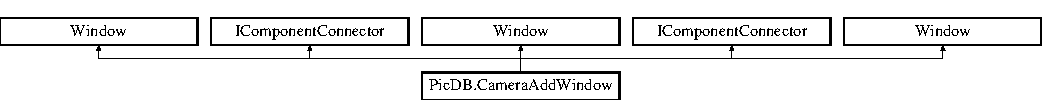
\includegraphics[height=1.317647cm]{class_pic_d_b_1_1_camera_add_window}
\end{center}
\end{figure}
\subsection*{Public Member Functions}
\begin{DoxyCompactItemize}
\item 
\mbox{\Hypertarget{class_pic_d_b_1_1_camera_add_window_ace6208321cbab35882ee466e5d73a40a}\label{class_pic_d_b_1_1_camera_add_window_ace6208321cbab35882ee466e5d73a40a}} 
{\bfseries Camera\+Add\+Window} (\mbox{\hyperlink{class_pic_d_b_1_1_view_models_1_1_main_window_view_model}{Main\+Window\+View\+Model}} controller)
\item 
void \mbox{\hyperlink{class_pic_d_b_1_1_camera_add_window_abb17f3480dce6c490f858d9f5e65ec8b}{Initialize\+Component}} ()
\begin{DoxyCompactList}\small\item\em Initialize\+Component \end{DoxyCompactList}\item 
void \mbox{\hyperlink{class_pic_d_b_1_1_camera_add_window_abb17f3480dce6c490f858d9f5e65ec8b}{Initialize\+Component}} ()
\begin{DoxyCompactList}\small\item\em Initialize\+Component \end{DoxyCompactList}\end{DoxyCompactItemize}


\subsection{Detailed Description}
Interaction logic for Camera\+Add\+Window.\+xaml 

\mbox{\hyperlink{class_pic_d_b_1_1_camera_add_window}{Camera\+Add\+Window}} 

\subsection{Member Function Documentation}
\mbox{\Hypertarget{class_pic_d_b_1_1_camera_add_window_abb17f3480dce6c490f858d9f5e65ec8b}\label{class_pic_d_b_1_1_camera_add_window_abb17f3480dce6c490f858d9f5e65ec8b}} 
\index{Pic\+D\+B\+::\+Camera\+Add\+Window@{Pic\+D\+B\+::\+Camera\+Add\+Window}!Initialize\+Component@{Initialize\+Component}}
\index{Initialize\+Component@{Initialize\+Component}!Pic\+D\+B\+::\+Camera\+Add\+Window@{Pic\+D\+B\+::\+Camera\+Add\+Window}}
\subsubsection{\texorpdfstring{Initialize\+Component()}{InitializeComponent()}\hspace{0.1cm}{\footnotesize\ttfamily [1/2]}}
{\footnotesize\ttfamily void Pic\+D\+B.\+Camera\+Add\+Window.\+Initialize\+Component (\begin{DoxyParamCaption}{ }\end{DoxyParamCaption})}



Initialize\+Component 

\mbox{\Hypertarget{class_pic_d_b_1_1_camera_add_window_abb17f3480dce6c490f858d9f5e65ec8b}\label{class_pic_d_b_1_1_camera_add_window_abb17f3480dce6c490f858d9f5e65ec8b}} 
\index{Pic\+D\+B\+::\+Camera\+Add\+Window@{Pic\+D\+B\+::\+Camera\+Add\+Window}!Initialize\+Component@{Initialize\+Component}}
\index{Initialize\+Component@{Initialize\+Component}!Pic\+D\+B\+::\+Camera\+Add\+Window@{Pic\+D\+B\+::\+Camera\+Add\+Window}}
\subsubsection{\texorpdfstring{Initialize\+Component()}{InitializeComponent()}\hspace{0.1cm}{\footnotesize\ttfamily [2/2]}}
{\footnotesize\ttfamily void Pic\+D\+B.\+Camera\+Add\+Window.\+Initialize\+Component (\begin{DoxyParamCaption}{ }\end{DoxyParamCaption})}



Initialize\+Component 



The documentation for this class was generated from the following files\+:\begin{DoxyCompactItemize}
\item 
C\+:/\+A\+A\+A-\/\+Technikum\+\_\+\+B\+W\+I/fourth\+Semester/\+S\+W\+E2/\+S\+W\+E2-\/\+C\+S/\+Pic\+D\+B/Camera\+Add\+Window.\+xaml.\+cs\item 
C\+:/\+A\+A\+A-\/\+Technikum\+\_\+\+B\+W\+I/fourth\+Semester/\+S\+W\+E2/\+S\+W\+E2-\/\+C\+S/\+Pic\+D\+B/obj/x86/\+Debug/Camera\+Add\+Window.\+g.\+cs\item 
C\+:/\+A\+A\+A-\/\+Technikum\+\_\+\+B\+W\+I/fourth\+Semester/\+S\+W\+E2/\+S\+W\+E2-\/\+C\+S/\+Pic\+D\+B/obj/x86/\+Debug/Camera\+Add\+Window.\+g.\+i.\+cs\end{DoxyCompactItemize}

\hypertarget{class_pic_d_b_1_1_view_models_1_1_camera_list_view_model}{}\section{Pic\+D\+B.\+View\+Models.\+Camera\+List\+View\+Model Class Reference}
\label{class_pic_d_b_1_1_view_models_1_1_camera_list_view_model}\index{Pic\+D\+B.\+View\+Models.\+Camera\+List\+View\+Model@{Pic\+D\+B.\+View\+Models.\+Camera\+List\+View\+Model}}


A viewmodel of all cameras  


Inheritance diagram for Pic\+D\+B.\+View\+Models.\+Camera\+List\+View\+Model\+:\begin{figure}[H]
\begin{center}
\leavevmode
\includegraphics[height=3.000000cm]{class_pic_d_b_1_1_view_models_1_1_camera_list_view_model}
\end{center}
\end{figure}
\subsection*{Public Member Functions}
\begin{DoxyCompactItemize}
\item 
void \mbox{\hyperlink{class_pic_d_b_1_1_view_models_1_1_camera_list_view_model_a7bf15c41092b0fb555a5b0943bc81807}{Synchronize\+Cameras}} ()
\begin{DoxyCompactList}\small\item\em Synchronizes all cameras to the UI \end{DoxyCompactList}\end{DoxyCompactItemize}
\subsection*{Properties}
\begin{DoxyCompactItemize}
\item 
I\+Enumerable$<$ I\+Camera\+View\+Model $>$ \mbox{\hyperlink{class_pic_d_b_1_1_view_models_1_1_camera_list_view_model_a7848fd33611b1899274874b8ff78e792}{List}}\hspace{0.3cm}{\ttfamily  \mbox{[}get\mbox{]}}
\begin{DoxyCompactList}\small\item\em A list of all Camera\+View\+Models \end{DoxyCompactList}\item 
I\+Camera\+View\+Model \mbox{\hyperlink{class_pic_d_b_1_1_view_models_1_1_camera_list_view_model_a757a0c21bba1b4653fd9d43cb396afae}{Current\+Camera}}\hspace{0.3cm}{\ttfamily  \mbox{[}get, set\mbox{]}}
\begin{DoxyCompactList}\small\item\em Reference to the currently selected camera in the UI \end{DoxyCompactList}\end{DoxyCompactItemize}
\subsection*{Additional Inherited Members}


\subsection{Detailed Description}
A viewmodel of all cameras 



\subsection{Member Function Documentation}
\mbox{\Hypertarget{class_pic_d_b_1_1_view_models_1_1_camera_list_view_model_a7bf15c41092b0fb555a5b0943bc81807}\label{class_pic_d_b_1_1_view_models_1_1_camera_list_view_model_a7bf15c41092b0fb555a5b0943bc81807}} 
\index{Pic\+D\+B\+::\+View\+Models\+::\+Camera\+List\+View\+Model@{Pic\+D\+B\+::\+View\+Models\+::\+Camera\+List\+View\+Model}!Synchronize\+Cameras@{Synchronize\+Cameras}}
\index{Synchronize\+Cameras@{Synchronize\+Cameras}!Pic\+D\+B\+::\+View\+Models\+::\+Camera\+List\+View\+Model@{Pic\+D\+B\+::\+View\+Models\+::\+Camera\+List\+View\+Model}}
\subsubsection{\texorpdfstring{Synchronize\+Cameras()}{SynchronizeCameras()}}
{\footnotesize\ttfamily void Pic\+D\+B.\+View\+Models.\+Camera\+List\+View\+Model.\+Synchronize\+Cameras (\begin{DoxyParamCaption}{ }\end{DoxyParamCaption})}



Synchronizes all cameras to the UI 



\subsection{Property Documentation}
\mbox{\Hypertarget{class_pic_d_b_1_1_view_models_1_1_camera_list_view_model_a757a0c21bba1b4653fd9d43cb396afae}\label{class_pic_d_b_1_1_view_models_1_1_camera_list_view_model_a757a0c21bba1b4653fd9d43cb396afae}} 
\index{Pic\+D\+B\+::\+View\+Models\+::\+Camera\+List\+View\+Model@{Pic\+D\+B\+::\+View\+Models\+::\+Camera\+List\+View\+Model}!Current\+Camera@{Current\+Camera}}
\index{Current\+Camera@{Current\+Camera}!Pic\+D\+B\+::\+View\+Models\+::\+Camera\+List\+View\+Model@{Pic\+D\+B\+::\+View\+Models\+::\+Camera\+List\+View\+Model}}
\subsubsection{\texorpdfstring{Current\+Camera}{CurrentCamera}}
{\footnotesize\ttfamily I\+Camera\+View\+Model Pic\+D\+B.\+View\+Models.\+Camera\+List\+View\+Model.\+Current\+Camera\hspace{0.3cm}{\ttfamily [get]}, {\ttfamily [set]}}



Reference to the currently selected camera in the UI 

\mbox{\Hypertarget{class_pic_d_b_1_1_view_models_1_1_camera_list_view_model_a7848fd33611b1899274874b8ff78e792}\label{class_pic_d_b_1_1_view_models_1_1_camera_list_view_model_a7848fd33611b1899274874b8ff78e792}} 
\index{Pic\+D\+B\+::\+View\+Models\+::\+Camera\+List\+View\+Model@{Pic\+D\+B\+::\+View\+Models\+::\+Camera\+List\+View\+Model}!List@{List}}
\index{List@{List}!Pic\+D\+B\+::\+View\+Models\+::\+Camera\+List\+View\+Model@{Pic\+D\+B\+::\+View\+Models\+::\+Camera\+List\+View\+Model}}
\subsubsection{\texorpdfstring{List}{List}}
{\footnotesize\ttfamily I\+Enumerable$<$I\+Camera\+View\+Model$>$ Pic\+D\+B.\+View\+Models.\+Camera\+List\+View\+Model.\+List\hspace{0.3cm}{\ttfamily [get]}}



A list of all Camera\+View\+Models 



The documentation for this class was generated from the following file\+:\begin{DoxyCompactItemize}
\item 
C\+:/\+A\+A\+A-\/\+Technikum\+\_\+\+B\+W\+I/fourth\+Semester/\+S\+W\+E2/\+S\+W\+E2-\/\+C\+S/\+Pic\+D\+B/\+View\+Models/Camera\+List\+View\+Model.\+cs\end{DoxyCompactItemize}

\hypertarget{class_pic_d_b_1_1_models_1_1_camera_model}{}\section{Pic\+D\+B.\+Models.\+Camera\+Model Class Reference}
\label{class_pic_d_b_1_1_models_1_1_camera_model}\index{Pic\+D\+B.\+Models.\+Camera\+Model@{Pic\+D\+B.\+Models.\+Camera\+Model}}


The model of a camera  


Inheritance diagram for Pic\+D\+B.\+Models.\+Camera\+Model\+:\begin{figure}[H]
\begin{center}
\leavevmode
\includegraphics[height=2.000000cm]{class_pic_d_b_1_1_models_1_1_camera_model}
\end{center}
\end{figure}
\subsection*{Public Member Functions}
\begin{DoxyCompactItemize}
\item 
\mbox{\Hypertarget{class_pic_d_b_1_1_models_1_1_camera_model_a0dad4b416044ad3b261aad2f210f6fef}\label{class_pic_d_b_1_1_models_1_1_camera_model_a0dad4b416044ad3b261aad2f210f6fef}} 
{\bfseries Camera\+Model} (int \mbox{\hyperlink{class_pic_d_b_1_1_models_1_1_camera_model_a31394a505a536d6c692e4fc4b76213f4}{ID}})
\item 
\mbox{\Hypertarget{class_pic_d_b_1_1_models_1_1_camera_model_a0c1ef897645616cef13e6a23c17e9105}\label{class_pic_d_b_1_1_models_1_1_camera_model_a0c1ef897645616cef13e6a23c17e9105}} 
{\bfseries Camera\+Model} (string producer, string make)
\item 
\mbox{\Hypertarget{class_pic_d_b_1_1_models_1_1_camera_model_a9c85f6901c6b6cb557d05075590604cb}\label{class_pic_d_b_1_1_models_1_1_camera_model_a9c85f6901c6b6cb557d05075590604cb}} 
{\bfseries Camera\+Model} (I\+Camera\+View\+Model view\+Model)
\end{DoxyCompactItemize}
\subsection*{Properties}
\begin{DoxyCompactItemize}
\item 
int \mbox{\hyperlink{class_pic_d_b_1_1_models_1_1_camera_model_a31394a505a536d6c692e4fc4b76213f4}{ID}}\hspace{0.3cm}{\ttfamily  \mbox{[}get, set\mbox{]}}
\begin{DoxyCompactList}\small\item\em ID of a camera (has to match with database) \end{DoxyCompactList}\item 
string \mbox{\hyperlink{class_pic_d_b_1_1_models_1_1_camera_model_a95db2c039e55aced4faa69e95ce8423a}{Producer}}\hspace{0.3cm}{\ttfamily  \mbox{[}get, set\mbox{]}}
\begin{DoxyCompactList}\small\item\em Producer of a camera \end{DoxyCompactList}\item 
string \mbox{\hyperlink{class_pic_d_b_1_1_models_1_1_camera_model_a7ab050807d92e1a2d5c6f6124b9c9b87}{Make}}\hspace{0.3cm}{\ttfamily  \mbox{[}get, set\mbox{]}}
\begin{DoxyCompactList}\small\item\em Make of a camera \end{DoxyCompactList}\item 
Date\+Time \mbox{\hyperlink{class_pic_d_b_1_1_models_1_1_camera_model_a553208926883eeab6ef3b58d031e480c}{Bought\+On}}\hspace{0.3cm}{\ttfamily  \mbox{[}get, set\mbox{]}}
\begin{DoxyCompactList}\small\item\em Datetime this camera has been bought on. \end{DoxyCompactList}\item 
string \mbox{\hyperlink{class_pic_d_b_1_1_models_1_1_camera_model_abc8338ceef1715e0bc03b842b692d43f}{Notes}}\hspace{0.3cm}{\ttfamily  \mbox{[}get, set\mbox{]}}
\begin{DoxyCompactList}\small\item\em Notes about the camera, eg.\+: \textquotesingle{}Makes very nice photographs in plain sunlight\textquotesingle{} \end{DoxyCompactList}\item 
decimal \mbox{\hyperlink{class_pic_d_b_1_1_models_1_1_camera_model_a2131f8ede10d20d95d3c2c9bb18bcfa6}{I\+S\+O\+Limit\+Good}}\hspace{0.3cm}{\ttfamily  \mbox{[}get, set\mbox{]}}
\begin{DoxyCompactList}\small\item\em Which I\+SO limit a camera has to surpass to be considered good \end{DoxyCompactList}\item 
decimal \mbox{\hyperlink{class_pic_d_b_1_1_models_1_1_camera_model_af5e0a52cbf9dc9f294c302b0525802ac}{I\+S\+O\+Limit\+Acceptable}}\hspace{0.3cm}{\ttfamily  \mbox{[}get, set\mbox{]}}
\begin{DoxyCompactList}\small\item\em Which I\+SO limit is deemed still acceptable \end{DoxyCompactList}\end{DoxyCompactItemize}


\subsection{Detailed Description}
The model of a camera 



\subsection{Property Documentation}
\mbox{\Hypertarget{class_pic_d_b_1_1_models_1_1_camera_model_a553208926883eeab6ef3b58d031e480c}\label{class_pic_d_b_1_1_models_1_1_camera_model_a553208926883eeab6ef3b58d031e480c}} 
\index{Pic\+D\+B\+::\+Models\+::\+Camera\+Model@{Pic\+D\+B\+::\+Models\+::\+Camera\+Model}!Bought\+On@{Bought\+On}}
\index{Bought\+On@{Bought\+On}!Pic\+D\+B\+::\+Models\+::\+Camera\+Model@{Pic\+D\+B\+::\+Models\+::\+Camera\+Model}}
\subsubsection{\texorpdfstring{Bought\+On}{BoughtOn}}
{\footnotesize\ttfamily Date\+Time Pic\+D\+B.\+Models.\+Camera\+Model.\+Bought\+On\hspace{0.3cm}{\ttfamily [get]}, {\ttfamily [set]}}



Datetime this camera has been bought on. 

\mbox{\Hypertarget{class_pic_d_b_1_1_models_1_1_camera_model_a31394a505a536d6c692e4fc4b76213f4}\label{class_pic_d_b_1_1_models_1_1_camera_model_a31394a505a536d6c692e4fc4b76213f4}} 
\index{Pic\+D\+B\+::\+Models\+::\+Camera\+Model@{Pic\+D\+B\+::\+Models\+::\+Camera\+Model}!ID@{ID}}
\index{ID@{ID}!Pic\+D\+B\+::\+Models\+::\+Camera\+Model@{Pic\+D\+B\+::\+Models\+::\+Camera\+Model}}
\subsubsection{\texorpdfstring{ID}{ID}}
{\footnotesize\ttfamily int Pic\+D\+B.\+Models.\+Camera\+Model.\+ID\hspace{0.3cm}{\ttfamily [get]}, {\ttfamily [set]}}



ID of a camera (has to match with database) 

\mbox{\Hypertarget{class_pic_d_b_1_1_models_1_1_camera_model_af5e0a52cbf9dc9f294c302b0525802ac}\label{class_pic_d_b_1_1_models_1_1_camera_model_af5e0a52cbf9dc9f294c302b0525802ac}} 
\index{Pic\+D\+B\+::\+Models\+::\+Camera\+Model@{Pic\+D\+B\+::\+Models\+::\+Camera\+Model}!I\+S\+O\+Limit\+Acceptable@{I\+S\+O\+Limit\+Acceptable}}
\index{I\+S\+O\+Limit\+Acceptable@{I\+S\+O\+Limit\+Acceptable}!Pic\+D\+B\+::\+Models\+::\+Camera\+Model@{Pic\+D\+B\+::\+Models\+::\+Camera\+Model}}
\subsubsection{\texorpdfstring{I\+S\+O\+Limit\+Acceptable}{ISOLimitAcceptable}}
{\footnotesize\ttfamily decimal Pic\+D\+B.\+Models.\+Camera\+Model.\+I\+S\+O\+Limit\+Acceptable\hspace{0.3cm}{\ttfamily [get]}, {\ttfamily [set]}}



Which I\+SO limit is deemed still acceptable 

\mbox{\Hypertarget{class_pic_d_b_1_1_models_1_1_camera_model_a2131f8ede10d20d95d3c2c9bb18bcfa6}\label{class_pic_d_b_1_1_models_1_1_camera_model_a2131f8ede10d20d95d3c2c9bb18bcfa6}} 
\index{Pic\+D\+B\+::\+Models\+::\+Camera\+Model@{Pic\+D\+B\+::\+Models\+::\+Camera\+Model}!I\+S\+O\+Limit\+Good@{I\+S\+O\+Limit\+Good}}
\index{I\+S\+O\+Limit\+Good@{I\+S\+O\+Limit\+Good}!Pic\+D\+B\+::\+Models\+::\+Camera\+Model@{Pic\+D\+B\+::\+Models\+::\+Camera\+Model}}
\subsubsection{\texorpdfstring{I\+S\+O\+Limit\+Good}{ISOLimitGood}}
{\footnotesize\ttfamily decimal Pic\+D\+B.\+Models.\+Camera\+Model.\+I\+S\+O\+Limit\+Good\hspace{0.3cm}{\ttfamily [get]}, {\ttfamily [set]}}



Which I\+SO limit a camera has to surpass to be considered good 

\mbox{\Hypertarget{class_pic_d_b_1_1_models_1_1_camera_model_a7ab050807d92e1a2d5c6f6124b9c9b87}\label{class_pic_d_b_1_1_models_1_1_camera_model_a7ab050807d92e1a2d5c6f6124b9c9b87}} 
\index{Pic\+D\+B\+::\+Models\+::\+Camera\+Model@{Pic\+D\+B\+::\+Models\+::\+Camera\+Model}!Make@{Make}}
\index{Make@{Make}!Pic\+D\+B\+::\+Models\+::\+Camera\+Model@{Pic\+D\+B\+::\+Models\+::\+Camera\+Model}}
\subsubsection{\texorpdfstring{Make}{Make}}
{\footnotesize\ttfamily string Pic\+D\+B.\+Models.\+Camera\+Model.\+Make\hspace{0.3cm}{\ttfamily [get]}, {\ttfamily [set]}}



Make of a camera 

\mbox{\Hypertarget{class_pic_d_b_1_1_models_1_1_camera_model_abc8338ceef1715e0bc03b842b692d43f}\label{class_pic_d_b_1_1_models_1_1_camera_model_abc8338ceef1715e0bc03b842b692d43f}} 
\index{Pic\+D\+B\+::\+Models\+::\+Camera\+Model@{Pic\+D\+B\+::\+Models\+::\+Camera\+Model}!Notes@{Notes}}
\index{Notes@{Notes}!Pic\+D\+B\+::\+Models\+::\+Camera\+Model@{Pic\+D\+B\+::\+Models\+::\+Camera\+Model}}
\subsubsection{\texorpdfstring{Notes}{Notes}}
{\footnotesize\ttfamily string Pic\+D\+B.\+Models.\+Camera\+Model.\+Notes\hspace{0.3cm}{\ttfamily [get]}, {\ttfamily [set]}}



Notes about the camera, eg.\+: \textquotesingle{}Makes very nice photographs in plain sunlight\textquotesingle{} 

\mbox{\Hypertarget{class_pic_d_b_1_1_models_1_1_camera_model_a95db2c039e55aced4faa69e95ce8423a}\label{class_pic_d_b_1_1_models_1_1_camera_model_a95db2c039e55aced4faa69e95ce8423a}} 
\index{Pic\+D\+B\+::\+Models\+::\+Camera\+Model@{Pic\+D\+B\+::\+Models\+::\+Camera\+Model}!Producer@{Producer}}
\index{Producer@{Producer}!Pic\+D\+B\+::\+Models\+::\+Camera\+Model@{Pic\+D\+B\+::\+Models\+::\+Camera\+Model}}
\subsubsection{\texorpdfstring{Producer}{Producer}}
{\footnotesize\ttfamily string Pic\+D\+B.\+Models.\+Camera\+Model.\+Producer\hspace{0.3cm}{\ttfamily [get]}, {\ttfamily [set]}}



Producer of a camera 



The documentation for this class was generated from the following file\+:\begin{DoxyCompactItemize}
\item 
C\+:/\+A\+A\+A-\/\+Technikum\+\_\+\+B\+W\+I/fourth\+Semester/\+S\+W\+E2/\+S\+W\+E2-\/\+C\+S/\+Pic\+D\+B/\+Models/Camera\+Model.\+cs\end{DoxyCompactItemize}

\hypertarget{class_pic_d_b_1_1_view_models_1_1_camera_view_model}{}\section{Pic\+D\+B.\+View\+Models.\+Camera\+View\+Model Class Reference}
\label{class_pic_d_b_1_1_view_models_1_1_camera_view_model}\index{Pic\+D\+B.\+View\+Models.\+Camera\+View\+Model@{Pic\+D\+B.\+View\+Models.\+Camera\+View\+Model}}


A viewmodel of a camera  


Inheritance diagram for Pic\+D\+B.\+View\+Models.\+Camera\+View\+Model\+:\begin{figure}[H]
\begin{center}
\leavevmode
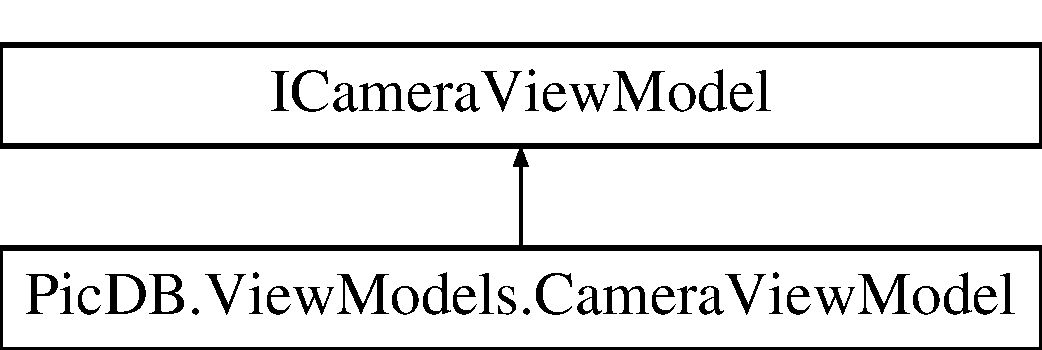
\includegraphics[height=2.000000cm]{class_pic_d_b_1_1_view_models_1_1_camera_view_model}
\end{center}
\end{figure}
\subsection*{Public Member Functions}
\begin{DoxyCompactItemize}
\item 
\mbox{\Hypertarget{class_pic_d_b_1_1_view_models_1_1_camera_view_model_a83b7d925f502fa3b732bf596175d9aa3}\label{class_pic_d_b_1_1_view_models_1_1_camera_view_model_a83b7d925f502fa3b732bf596175d9aa3}} 
{\bfseries Camera\+View\+Model} (I\+Camera\+Model model)
\item 
I\+S\+O\+Ratings \mbox{\hyperlink{class_pic_d_b_1_1_view_models_1_1_camera_view_model_a3e4639d271b4c240025e59b705de2a3e}{Translate\+I\+S\+O\+Rating}} (decimal iso)
\begin{DoxyCompactList}\small\item\em O\+B\+S\+O\+L\+E\+TE \end{DoxyCompactList}\end{DoxyCompactItemize}
\subsection*{Public Attributes}
\begin{DoxyCompactItemize}
\item 
int \mbox{\hyperlink{class_pic_d_b_1_1_view_models_1_1_camera_view_model_abc1f2929064a6db42c7d111be20a3cea}{Number\+Of\+Pictures}} =$>$ throw new Not\+Implemented\+Exception()
\begin{DoxyCompactList}\small\item\em O\+B\+S\+O\+L\+E\+TE \end{DoxyCompactList}\end{DoxyCompactItemize}
\subsection*{Properties}
\begin{DoxyCompactItemize}
\item 
int \mbox{\hyperlink{class_pic_d_b_1_1_view_models_1_1_camera_view_model_a013f0a6651a495227ed5bc449741e44b}{ID}}\hspace{0.3cm}{\ttfamily  \mbox{[}get, set\mbox{]}}
\begin{DoxyCompactList}\small\item\em Database primary key \end{DoxyCompactList}\item 
string \mbox{\hyperlink{class_pic_d_b_1_1_view_models_1_1_camera_view_model_a31cb4d872712b29ed463be66efa76af3}{Producer}}\hspace{0.3cm}{\ttfamily  \mbox{[}get, set\mbox{]}}
\begin{DoxyCompactList}\small\item\em Name of the producer \end{DoxyCompactList}\item 
string \mbox{\hyperlink{class_pic_d_b_1_1_view_models_1_1_camera_view_model_abd4cfc6713cf37ce8a3a11149b56b18d}{Make}}\hspace{0.3cm}{\ttfamily  \mbox{[}get, set\mbox{]}}
\begin{DoxyCompactList}\small\item\em Name of the camera \end{DoxyCompactList}\item 
Date\+Time \mbox{\hyperlink{class_pic_d_b_1_1_view_models_1_1_camera_view_model_ad99a2f3ac943e7bca895ecaab629c9b4}{Bought\+On}}\hspace{0.3cm}{\ttfamily  \mbox{[}get, set\mbox{]}}
\begin{DoxyCompactList}\small\item\em Datetime of buydate \end{DoxyCompactList}\item 
string \mbox{\hyperlink{class_pic_d_b_1_1_view_models_1_1_camera_view_model_acec285bd0efe751d421f2c905e720c4b}{Notes}}\hspace{0.3cm}{\ttfamily  \mbox{[}get, set\mbox{]}}
\begin{DoxyCompactList}\small\item\em Notes \end{DoxyCompactList}\item 
bool \mbox{\hyperlink{class_pic_d_b_1_1_view_models_1_1_camera_view_model_aa5c75f4e8a5484508253f3721b9ca3f1}{Is\+Valid}}\hspace{0.3cm}{\ttfamily  \mbox{[}get\mbox{]}}
\begin{DoxyCompactList}\small\item\em Checks if a camera viewmodel is valid \end{DoxyCompactList}\item 
string \mbox{\hyperlink{class_pic_d_b_1_1_view_models_1_1_camera_view_model_a6cb8ea52632e1e5aefd6a6e54691dbeb}{Validation\+Summary}}\hspace{0.3cm}{\ttfamily  \mbox{[}get\mbox{]}}
\begin{DoxyCompactList}\small\item\em Summary if validation check \end{DoxyCompactList}\item 
bool \mbox{\hyperlink{class_pic_d_b_1_1_view_models_1_1_camera_view_model_ad5b2a5bce051ecbfc1ae3754a3f8aa44}{Is\+Valid\+Producer}}\hspace{0.3cm}{\ttfamily  \mbox{[}get\mbox{]}}
\begin{DoxyCompactList}\small\item\em Checks if producer is valid \end{DoxyCompactList}\item 
bool \mbox{\hyperlink{class_pic_d_b_1_1_view_models_1_1_camera_view_model_ad9c951f992a386532ef5f512fd3e1ff0}{Is\+Valid\+Make}}\hspace{0.3cm}{\ttfamily  \mbox{[}get\mbox{]}}
\begin{DoxyCompactList}\small\item\em Checks if make is valid \end{DoxyCompactList}\item 
bool \mbox{\hyperlink{class_pic_d_b_1_1_view_models_1_1_camera_view_model_a74319f7025c06dfb7978fa7fb5e7b162}{Is\+Valid\+Bought\+On}}\hspace{0.3cm}{\ttfamily  \mbox{[}get\mbox{]}}
\begin{DoxyCompactList}\small\item\em Checks if buydate is valid \end{DoxyCompactList}\item 
decimal \mbox{\hyperlink{class_pic_d_b_1_1_view_models_1_1_camera_view_model_a5b469c0b88da60e062ba0211973ae52d}{I\+S\+O\+Limit\+Good}}\hspace{0.3cm}{\ttfamily  \mbox{[}get, set\mbox{]}}
\begin{DoxyCompactList}\small\item\em Max I\+SO Value for good results. 0 means \char`\"{}not defined\char`\"{} \end{DoxyCompactList}\item 
decimal \mbox{\hyperlink{class_pic_d_b_1_1_view_models_1_1_camera_view_model_a128275fdf0e7d3951568987a003405eb}{I\+S\+O\+Limit\+Acceptable}}\hspace{0.3cm}{\ttfamily  \mbox{[}get, set\mbox{]}}
\begin{DoxyCompactList}\small\item\em Max I\+SO Value for acceptable results. 0 means \char`\"{}not defined\char`\"{} \end{DoxyCompactList}\end{DoxyCompactItemize}


\subsection{Detailed Description}
A viewmodel of a camera 



\subsection{Member Function Documentation}
\mbox{\Hypertarget{class_pic_d_b_1_1_view_models_1_1_camera_view_model_a3e4639d271b4c240025e59b705de2a3e}\label{class_pic_d_b_1_1_view_models_1_1_camera_view_model_a3e4639d271b4c240025e59b705de2a3e}} 
\index{Pic\+D\+B\+::\+View\+Models\+::\+Camera\+View\+Model@{Pic\+D\+B\+::\+View\+Models\+::\+Camera\+View\+Model}!Translate\+I\+S\+O\+Rating@{Translate\+I\+S\+O\+Rating}}
\index{Translate\+I\+S\+O\+Rating@{Translate\+I\+S\+O\+Rating}!Pic\+D\+B\+::\+View\+Models\+::\+Camera\+View\+Model@{Pic\+D\+B\+::\+View\+Models\+::\+Camera\+View\+Model}}
\subsubsection{\texorpdfstring{Translate\+I\+S\+O\+Rating()}{TranslateISORating()}}
{\footnotesize\ttfamily I\+S\+O\+Ratings Pic\+D\+B.\+View\+Models.\+Camera\+View\+Model.\+Translate\+I\+S\+O\+Rating (\begin{DoxyParamCaption}\item[{decimal}]{iso }\end{DoxyParamCaption})}



O\+B\+S\+O\+L\+E\+TE 


\begin{DoxyParams}{Parameters}
{\em iso} & \\
\hline
\end{DoxyParams}
\begin{DoxyReturn}{Returns}

\end{DoxyReturn}


\subsection{Member Data Documentation}
\mbox{\Hypertarget{class_pic_d_b_1_1_view_models_1_1_camera_view_model_abc1f2929064a6db42c7d111be20a3cea}\label{class_pic_d_b_1_1_view_models_1_1_camera_view_model_abc1f2929064a6db42c7d111be20a3cea}} 
\index{Pic\+D\+B\+::\+View\+Models\+::\+Camera\+View\+Model@{Pic\+D\+B\+::\+View\+Models\+::\+Camera\+View\+Model}!Number\+Of\+Pictures@{Number\+Of\+Pictures}}
\index{Number\+Of\+Pictures@{Number\+Of\+Pictures}!Pic\+D\+B\+::\+View\+Models\+::\+Camera\+View\+Model@{Pic\+D\+B\+::\+View\+Models\+::\+Camera\+View\+Model}}
\subsubsection{\texorpdfstring{Number\+Of\+Pictures}{NumberOfPictures}}
{\footnotesize\ttfamily int Pic\+D\+B.\+View\+Models.\+Camera\+View\+Model.\+Number\+Of\+Pictures =$>$ throw new Not\+Implemented\+Exception()}



O\+B\+S\+O\+L\+E\+TE 



\subsection{Property Documentation}
\mbox{\Hypertarget{class_pic_d_b_1_1_view_models_1_1_camera_view_model_ad99a2f3ac943e7bca895ecaab629c9b4}\label{class_pic_d_b_1_1_view_models_1_1_camera_view_model_ad99a2f3ac943e7bca895ecaab629c9b4}} 
\index{Pic\+D\+B\+::\+View\+Models\+::\+Camera\+View\+Model@{Pic\+D\+B\+::\+View\+Models\+::\+Camera\+View\+Model}!Bought\+On@{Bought\+On}}
\index{Bought\+On@{Bought\+On}!Pic\+D\+B\+::\+View\+Models\+::\+Camera\+View\+Model@{Pic\+D\+B\+::\+View\+Models\+::\+Camera\+View\+Model}}
\subsubsection{\texorpdfstring{Bought\+On}{BoughtOn}}
{\footnotesize\ttfamily Date\+Time Pic\+D\+B.\+View\+Models.\+Camera\+View\+Model.\+Bought\+On\hspace{0.3cm}{\ttfamily [get]}, {\ttfamily [set]}}



Datetime of buydate 

\mbox{\Hypertarget{class_pic_d_b_1_1_view_models_1_1_camera_view_model_a013f0a6651a495227ed5bc449741e44b}\label{class_pic_d_b_1_1_view_models_1_1_camera_view_model_a013f0a6651a495227ed5bc449741e44b}} 
\index{Pic\+D\+B\+::\+View\+Models\+::\+Camera\+View\+Model@{Pic\+D\+B\+::\+View\+Models\+::\+Camera\+View\+Model}!ID@{ID}}
\index{ID@{ID}!Pic\+D\+B\+::\+View\+Models\+::\+Camera\+View\+Model@{Pic\+D\+B\+::\+View\+Models\+::\+Camera\+View\+Model}}
\subsubsection{\texorpdfstring{ID}{ID}}
{\footnotesize\ttfamily int Pic\+D\+B.\+View\+Models.\+Camera\+View\+Model.\+ID\hspace{0.3cm}{\ttfamily [get]}, {\ttfamily [set]}}



Database primary key 

\mbox{\Hypertarget{class_pic_d_b_1_1_view_models_1_1_camera_view_model_a128275fdf0e7d3951568987a003405eb}\label{class_pic_d_b_1_1_view_models_1_1_camera_view_model_a128275fdf0e7d3951568987a003405eb}} 
\index{Pic\+D\+B\+::\+View\+Models\+::\+Camera\+View\+Model@{Pic\+D\+B\+::\+View\+Models\+::\+Camera\+View\+Model}!I\+S\+O\+Limit\+Acceptable@{I\+S\+O\+Limit\+Acceptable}}
\index{I\+S\+O\+Limit\+Acceptable@{I\+S\+O\+Limit\+Acceptable}!Pic\+D\+B\+::\+View\+Models\+::\+Camera\+View\+Model@{Pic\+D\+B\+::\+View\+Models\+::\+Camera\+View\+Model}}
\subsubsection{\texorpdfstring{I\+S\+O\+Limit\+Acceptable}{ISOLimitAcceptable}}
{\footnotesize\ttfamily decimal Pic\+D\+B.\+View\+Models.\+Camera\+View\+Model.\+I\+S\+O\+Limit\+Acceptable\hspace{0.3cm}{\ttfamily [get]}, {\ttfamily [set]}}



Max I\+SO Value for acceptable results. 0 means \char`\"{}not defined\char`\"{} 

\mbox{\Hypertarget{class_pic_d_b_1_1_view_models_1_1_camera_view_model_a5b469c0b88da60e062ba0211973ae52d}\label{class_pic_d_b_1_1_view_models_1_1_camera_view_model_a5b469c0b88da60e062ba0211973ae52d}} 
\index{Pic\+D\+B\+::\+View\+Models\+::\+Camera\+View\+Model@{Pic\+D\+B\+::\+View\+Models\+::\+Camera\+View\+Model}!I\+S\+O\+Limit\+Good@{I\+S\+O\+Limit\+Good}}
\index{I\+S\+O\+Limit\+Good@{I\+S\+O\+Limit\+Good}!Pic\+D\+B\+::\+View\+Models\+::\+Camera\+View\+Model@{Pic\+D\+B\+::\+View\+Models\+::\+Camera\+View\+Model}}
\subsubsection{\texorpdfstring{I\+S\+O\+Limit\+Good}{ISOLimitGood}}
{\footnotesize\ttfamily decimal Pic\+D\+B.\+View\+Models.\+Camera\+View\+Model.\+I\+S\+O\+Limit\+Good\hspace{0.3cm}{\ttfamily [get]}, {\ttfamily [set]}}



Max I\+SO Value for good results. 0 means \char`\"{}not defined\char`\"{} 

\mbox{\Hypertarget{class_pic_d_b_1_1_view_models_1_1_camera_view_model_aa5c75f4e8a5484508253f3721b9ca3f1}\label{class_pic_d_b_1_1_view_models_1_1_camera_view_model_aa5c75f4e8a5484508253f3721b9ca3f1}} 
\index{Pic\+D\+B\+::\+View\+Models\+::\+Camera\+View\+Model@{Pic\+D\+B\+::\+View\+Models\+::\+Camera\+View\+Model}!Is\+Valid@{Is\+Valid}}
\index{Is\+Valid@{Is\+Valid}!Pic\+D\+B\+::\+View\+Models\+::\+Camera\+View\+Model@{Pic\+D\+B\+::\+View\+Models\+::\+Camera\+View\+Model}}
\subsubsection{\texorpdfstring{Is\+Valid}{IsValid}}
{\footnotesize\ttfamily bool Pic\+D\+B.\+View\+Models.\+Camera\+View\+Model.\+Is\+Valid\hspace{0.3cm}{\ttfamily [get]}}



Checks if a camera viewmodel is valid 

\mbox{\Hypertarget{class_pic_d_b_1_1_view_models_1_1_camera_view_model_a74319f7025c06dfb7978fa7fb5e7b162}\label{class_pic_d_b_1_1_view_models_1_1_camera_view_model_a74319f7025c06dfb7978fa7fb5e7b162}} 
\index{Pic\+D\+B\+::\+View\+Models\+::\+Camera\+View\+Model@{Pic\+D\+B\+::\+View\+Models\+::\+Camera\+View\+Model}!Is\+Valid\+Bought\+On@{Is\+Valid\+Bought\+On}}
\index{Is\+Valid\+Bought\+On@{Is\+Valid\+Bought\+On}!Pic\+D\+B\+::\+View\+Models\+::\+Camera\+View\+Model@{Pic\+D\+B\+::\+View\+Models\+::\+Camera\+View\+Model}}
\subsubsection{\texorpdfstring{Is\+Valid\+Bought\+On}{IsValidBoughtOn}}
{\footnotesize\ttfamily bool Pic\+D\+B.\+View\+Models.\+Camera\+View\+Model.\+Is\+Valid\+Bought\+On\hspace{0.3cm}{\ttfamily [get]}}



Checks if buydate is valid 

\mbox{\Hypertarget{class_pic_d_b_1_1_view_models_1_1_camera_view_model_ad9c951f992a386532ef5f512fd3e1ff0}\label{class_pic_d_b_1_1_view_models_1_1_camera_view_model_ad9c951f992a386532ef5f512fd3e1ff0}} 
\index{Pic\+D\+B\+::\+View\+Models\+::\+Camera\+View\+Model@{Pic\+D\+B\+::\+View\+Models\+::\+Camera\+View\+Model}!Is\+Valid\+Make@{Is\+Valid\+Make}}
\index{Is\+Valid\+Make@{Is\+Valid\+Make}!Pic\+D\+B\+::\+View\+Models\+::\+Camera\+View\+Model@{Pic\+D\+B\+::\+View\+Models\+::\+Camera\+View\+Model}}
\subsubsection{\texorpdfstring{Is\+Valid\+Make}{IsValidMake}}
{\footnotesize\ttfamily bool Pic\+D\+B.\+View\+Models.\+Camera\+View\+Model.\+Is\+Valid\+Make\hspace{0.3cm}{\ttfamily [get]}}



Checks if make is valid 

\mbox{\Hypertarget{class_pic_d_b_1_1_view_models_1_1_camera_view_model_ad5b2a5bce051ecbfc1ae3754a3f8aa44}\label{class_pic_d_b_1_1_view_models_1_1_camera_view_model_ad5b2a5bce051ecbfc1ae3754a3f8aa44}} 
\index{Pic\+D\+B\+::\+View\+Models\+::\+Camera\+View\+Model@{Pic\+D\+B\+::\+View\+Models\+::\+Camera\+View\+Model}!Is\+Valid\+Producer@{Is\+Valid\+Producer}}
\index{Is\+Valid\+Producer@{Is\+Valid\+Producer}!Pic\+D\+B\+::\+View\+Models\+::\+Camera\+View\+Model@{Pic\+D\+B\+::\+View\+Models\+::\+Camera\+View\+Model}}
\subsubsection{\texorpdfstring{Is\+Valid\+Producer}{IsValidProducer}}
{\footnotesize\ttfamily bool Pic\+D\+B.\+View\+Models.\+Camera\+View\+Model.\+Is\+Valid\+Producer\hspace{0.3cm}{\ttfamily [get]}}



Checks if producer is valid 

\mbox{\Hypertarget{class_pic_d_b_1_1_view_models_1_1_camera_view_model_abd4cfc6713cf37ce8a3a11149b56b18d}\label{class_pic_d_b_1_1_view_models_1_1_camera_view_model_abd4cfc6713cf37ce8a3a11149b56b18d}} 
\index{Pic\+D\+B\+::\+View\+Models\+::\+Camera\+View\+Model@{Pic\+D\+B\+::\+View\+Models\+::\+Camera\+View\+Model}!Make@{Make}}
\index{Make@{Make}!Pic\+D\+B\+::\+View\+Models\+::\+Camera\+View\+Model@{Pic\+D\+B\+::\+View\+Models\+::\+Camera\+View\+Model}}
\subsubsection{\texorpdfstring{Make}{Make}}
{\footnotesize\ttfamily string Pic\+D\+B.\+View\+Models.\+Camera\+View\+Model.\+Make\hspace{0.3cm}{\ttfamily [get]}, {\ttfamily [set]}}



Name of the camera 

\mbox{\Hypertarget{class_pic_d_b_1_1_view_models_1_1_camera_view_model_acec285bd0efe751d421f2c905e720c4b}\label{class_pic_d_b_1_1_view_models_1_1_camera_view_model_acec285bd0efe751d421f2c905e720c4b}} 
\index{Pic\+D\+B\+::\+View\+Models\+::\+Camera\+View\+Model@{Pic\+D\+B\+::\+View\+Models\+::\+Camera\+View\+Model}!Notes@{Notes}}
\index{Notes@{Notes}!Pic\+D\+B\+::\+View\+Models\+::\+Camera\+View\+Model@{Pic\+D\+B\+::\+View\+Models\+::\+Camera\+View\+Model}}
\subsubsection{\texorpdfstring{Notes}{Notes}}
{\footnotesize\ttfamily string Pic\+D\+B.\+View\+Models.\+Camera\+View\+Model.\+Notes\hspace{0.3cm}{\ttfamily [get]}, {\ttfamily [set]}}



Notes 

\mbox{\Hypertarget{class_pic_d_b_1_1_view_models_1_1_camera_view_model_a31cb4d872712b29ed463be66efa76af3}\label{class_pic_d_b_1_1_view_models_1_1_camera_view_model_a31cb4d872712b29ed463be66efa76af3}} 
\index{Pic\+D\+B\+::\+View\+Models\+::\+Camera\+View\+Model@{Pic\+D\+B\+::\+View\+Models\+::\+Camera\+View\+Model}!Producer@{Producer}}
\index{Producer@{Producer}!Pic\+D\+B\+::\+View\+Models\+::\+Camera\+View\+Model@{Pic\+D\+B\+::\+View\+Models\+::\+Camera\+View\+Model}}
\subsubsection{\texorpdfstring{Producer}{Producer}}
{\footnotesize\ttfamily string Pic\+D\+B.\+View\+Models.\+Camera\+View\+Model.\+Producer\hspace{0.3cm}{\ttfamily [get]}, {\ttfamily [set]}}



Name of the producer 

\mbox{\Hypertarget{class_pic_d_b_1_1_view_models_1_1_camera_view_model_a6cb8ea52632e1e5aefd6a6e54691dbeb}\label{class_pic_d_b_1_1_view_models_1_1_camera_view_model_a6cb8ea52632e1e5aefd6a6e54691dbeb}} 
\index{Pic\+D\+B\+::\+View\+Models\+::\+Camera\+View\+Model@{Pic\+D\+B\+::\+View\+Models\+::\+Camera\+View\+Model}!Validation\+Summary@{Validation\+Summary}}
\index{Validation\+Summary@{Validation\+Summary}!Pic\+D\+B\+::\+View\+Models\+::\+Camera\+View\+Model@{Pic\+D\+B\+::\+View\+Models\+::\+Camera\+View\+Model}}
\subsubsection{\texorpdfstring{Validation\+Summary}{ValidationSummary}}
{\footnotesize\ttfamily string Pic\+D\+B.\+View\+Models.\+Camera\+View\+Model.\+Validation\+Summary\hspace{0.3cm}{\ttfamily [get]}}



Summary if validation check 



The documentation for this class was generated from the following file\+:\begin{DoxyCompactItemize}
\item 
C\+:/\+A\+A\+A-\/\+Technikum\+\_\+\+B\+W\+I/fourth\+Semester/\+S\+W\+E2/\+S\+W\+E2-\/\+C\+S/\+Pic\+D\+B/\+View\+Models/Camera\+View\+Model.\+cs\end{DoxyCompactItemize}

\hypertarget{class_pic_d_b_1_1_camera_window}{}\section{Pic\+D\+B.\+Camera\+Window Class Reference}
\label{class_pic_d_b_1_1_camera_window}\index{Pic\+D\+B.\+Camera\+Window@{Pic\+D\+B.\+Camera\+Window}}


Interaction logic for Camera\+Window.\+xaml  


Inheritance diagram for Pic\+D\+B.\+Camera\+Window\+:\begin{figure}[H]
\begin{center}
\leavevmode
\includegraphics[height=1.523810cm]{class_pic_d_b_1_1_camera_window}
\end{center}
\end{figure}
\subsection*{Public Member Functions}
\begin{DoxyCompactItemize}
\item 
\mbox{\Hypertarget{class_pic_d_b_1_1_camera_window_a3a7d76b4429c79da2323e391550b8701}\label{class_pic_d_b_1_1_camera_window_a3a7d76b4429c79da2323e391550b8701}} 
{\bfseries Camera\+Window} (\mbox{\hyperlink{class_pic_d_b_1_1_view_models_1_1_main_window_view_model}{Main\+Window\+View\+Model}} controller)
\item 
void \mbox{\hyperlink{class_pic_d_b_1_1_camera_window_a0f76da75ec227a474e47daa78d549653}{Initialize\+Component}} ()
\begin{DoxyCompactList}\small\item\em Initialize\+Component \end{DoxyCompactList}\item 
void \mbox{\hyperlink{class_pic_d_b_1_1_camera_window_a0f76da75ec227a474e47daa78d549653}{Initialize\+Component}} ()
\begin{DoxyCompactList}\small\item\em Initialize\+Component \end{DoxyCompactList}\end{DoxyCompactItemize}


\subsection{Detailed Description}
Interaction logic for Camera\+Window.\+xaml 

\mbox{\hyperlink{class_pic_d_b_1_1_camera_window}{Camera\+Window}} 

\subsection{Member Function Documentation}
\mbox{\Hypertarget{class_pic_d_b_1_1_camera_window_a0f76da75ec227a474e47daa78d549653}\label{class_pic_d_b_1_1_camera_window_a0f76da75ec227a474e47daa78d549653}} 
\index{Pic\+D\+B\+::\+Camera\+Window@{Pic\+D\+B\+::\+Camera\+Window}!Initialize\+Component@{Initialize\+Component}}
\index{Initialize\+Component@{Initialize\+Component}!Pic\+D\+B\+::\+Camera\+Window@{Pic\+D\+B\+::\+Camera\+Window}}
\subsubsection{\texorpdfstring{Initialize\+Component()}{InitializeComponent()}\hspace{0.1cm}{\footnotesize\ttfamily [1/2]}}
{\footnotesize\ttfamily void Pic\+D\+B.\+Camera\+Window.\+Initialize\+Component (\begin{DoxyParamCaption}{ }\end{DoxyParamCaption})}



Initialize\+Component 

\mbox{\Hypertarget{class_pic_d_b_1_1_camera_window_a0f76da75ec227a474e47daa78d549653}\label{class_pic_d_b_1_1_camera_window_a0f76da75ec227a474e47daa78d549653}} 
\index{Pic\+D\+B\+::\+Camera\+Window@{Pic\+D\+B\+::\+Camera\+Window}!Initialize\+Component@{Initialize\+Component}}
\index{Initialize\+Component@{Initialize\+Component}!Pic\+D\+B\+::\+Camera\+Window@{Pic\+D\+B\+::\+Camera\+Window}}
\subsubsection{\texorpdfstring{Initialize\+Component()}{InitializeComponent()}\hspace{0.1cm}{\footnotesize\ttfamily [2/2]}}
{\footnotesize\ttfamily void Pic\+D\+B.\+Camera\+Window.\+Initialize\+Component (\begin{DoxyParamCaption}{ }\end{DoxyParamCaption})}



Initialize\+Component 



The documentation for this class was generated from the following files\+:\begin{DoxyCompactItemize}
\item 
C\+:/\+A\+A\+A-\/\+Technikum\+\_\+\+B\+W\+I/fourth\+Semester/\+S\+W\+E2/\+S\+W\+E2-\/\+C\+S/\+Pic\+D\+B/Camera\+Window.\+xaml.\+cs\item 
C\+:/\+A\+A\+A-\/\+Technikum\+\_\+\+B\+W\+I/fourth\+Semester/\+S\+W\+E2/\+S\+W\+E2-\/\+C\+S/\+Pic\+D\+B/obj/x86/\+Debug/Camera\+Window.\+g.\+cs\item 
C\+:/\+A\+A\+A-\/\+Technikum\+\_\+\+B\+W\+I/fourth\+Semester/\+S\+W\+E2/\+S\+W\+E2-\/\+C\+S/\+Pic\+D\+B/obj/x86/\+Debug/Camera\+Window.\+g.\+i.\+cs\end{DoxyCompactItemize}

\hypertarget{class_pic_d_b_1_1_layers_1_1_data_access_layer}{}\section{Pic\+D\+B.\+Layers.\+Data\+Access\+Layer Class Reference}
\label{class_pic_d_b_1_1_layers_1_1_data_access_layer}\index{Pic\+D\+B.\+Layers.\+Data\+Access\+Layer@{Pic\+D\+B.\+Layers.\+Data\+Access\+Layer}}


Handles the access to the database.  


Inheritance diagram for Pic\+D\+B.\+Layers.\+Data\+Access\+Layer\+:\begin{figure}[H]
\begin{center}
\leavevmode
\includegraphics[height=2.000000cm]{class_pic_d_b_1_1_layers_1_1_data_access_layer}
\end{center}
\end{figure}
\subsection*{Public Member Functions}
\begin{DoxyCompactItemize}
\item 
\mbox{\hyperlink{class_pic_d_b_1_1_layers_1_1_data_access_layer_aa596817ac8c89272846f1a8196408178}{Data\+Access\+Layer}} ()
\begin{DoxyCompactList}\small\item\em In the constructor only the connection string based on the config file is being set. \end{DoxyCompactList}\item 
I\+Enumerable$<$ I\+Picture\+Model $>$ \mbox{\hyperlink{class_pic_d_b_1_1_layers_1_1_data_access_layer_a0866667e7f98fc65e29c5b1fce4eff84}{Get\+Pictures}} (string name\+Part, I\+Photographer\+Model photographer\+Parts, I\+I\+P\+T\+C\+Model iptc\+Parts, I\+E\+X\+I\+F\+Model exif\+Parts)
\begin{DoxyCompactList}\small\item\em Returns a list of A\+LL Pictures from the directory, based on a database query. \end{DoxyCompactList}\item 
I\+Picture\+Model \mbox{\hyperlink{class_pic_d_b_1_1_layers_1_1_data_access_layer_ac41c90cb91e0df488dc886db37fdc07b}{Get\+Picture}} (int ID)
\begin{DoxyCompactList}\small\item\em Returns O\+NE Picture from the database. \end{DoxyCompactList}\item 
void \mbox{\hyperlink{class_pic_d_b_1_1_layers_1_1_data_access_layer_a7fd40a4ce08e73fa15fd964138d95f20}{Save}} (I\+Picture\+Model picture)
\begin{DoxyCompactList}\small\item\em Saves all changes for one picture to the database. \end{DoxyCompactList}\item 
void \mbox{\hyperlink{class_pic_d_b_1_1_layers_1_1_data_access_layer_a503286ca6863223b52464ae483f1b9e3}{Delete\+Picture}} (int ID)
\begin{DoxyCompactList}\small\item\em Deletes a Picture from the database A\+ND from the file system. \end{DoxyCompactList}\item 
I\+Enumerable$<$ I\+Photographer\+Model $>$ \mbox{\hyperlink{class_pic_d_b_1_1_layers_1_1_data_access_layer_a41fdea4749eb2ff6826099bae90d0620}{Get\+Photographers}} ()
\begin{DoxyCompactList}\small\item\em Returns a list of A\+LL photographers, based on a database query. \end{DoxyCompactList}\item 
I\+Photographer\+Model \mbox{\hyperlink{class_pic_d_b_1_1_layers_1_1_data_access_layer_a1a5096b0ee7c2e9c8a051af5f74ad2ec}{Get\+Photographer}} (int ID)
\begin{DoxyCompactList}\small\item\em Returns a list of O\+NE photographers, based on a database query. \end{DoxyCompactList}\item 
void \mbox{\hyperlink{class_pic_d_b_1_1_layers_1_1_data_access_layer_a4e3554f691b1aae313a9c1162ccd3bee}{Save}} (I\+Photographer\+Model photographer)
\begin{DoxyCompactList}\small\item\em Saves all changes of one photographer to the database. \end{DoxyCompactList}\item 
void \mbox{\hyperlink{class_pic_d_b_1_1_layers_1_1_data_access_layer_abbdd8f6f2145b58a3c1b084d203510f6}{Delete\+Photographer}} (int ID)
\begin{DoxyCompactList}\small\item\em Deletes a photographer from database based on given ID \end{DoxyCompactList}\item 
I\+Enumerable$<$ I\+Camera\+Model $>$ \mbox{\hyperlink{class_pic_d_b_1_1_layers_1_1_data_access_layer_a0aef35ea518e7020dfeb77b9e7f556e9}{Get\+Cameras}} ()
\begin{DoxyCompactList}\small\item\em Returns a list of A\+LL Cameras. \end{DoxyCompactList}\item 
I\+Camera\+Model \mbox{\hyperlink{class_pic_d_b_1_1_layers_1_1_data_access_layer_a58aa8e9e53b9c7fdcacb48582daf9f36}{Get\+Camera}} (int ID)
\begin{DoxyCompactList}\small\item\em Returns O\+NE Camera \end{DoxyCompactList}\item 
void \mbox{\hyperlink{class_pic_d_b_1_1_layers_1_1_data_access_layer_a1909e4d371b56f0b5d400658ed0b167b}{Update\+Camera}} (I\+Camera\+Model camera\+Model)
\begin{DoxyCompactList}\small\item\em Updates O\+NE camera \end{DoxyCompactList}\item 
void \mbox{\hyperlink{class_pic_d_b_1_1_layers_1_1_data_access_layer_aae4b79abc6acf09649d528b31b1e3f17}{Delete\+Camera}} (int ID)
\begin{DoxyCompactList}\small\item\em Deletes O\+NE camera based on ID \end{DoxyCompactList}\item 
void \mbox{\hyperlink{class_pic_d_b_1_1_layers_1_1_data_access_layer_af7dbcbd6f4ef0058b7b33a052eca4c06}{Save\+Camera}} (\mbox{\hyperlink{class_pic_d_b_1_1_models_1_1_camera_model}{Camera\+Model}} camera)
\begin{DoxyCompactList}\small\item\em Saves a camera to the database \end{DoxyCompactList}\item 
void \mbox{\hyperlink{class_pic_d_b_1_1_layers_1_1_data_access_layer_a6b4baf032a0dc297b35f28ab2455b8f5}{Save\+Photographer}} (\mbox{\hyperlink{class_pic_d_b_1_1_models_1_1_photographer_model}{Photographer\+Model}} photographer)
\begin{DoxyCompactList}\small\item\em Saves a photographer to the database \end{DoxyCompactList}\item 
void \mbox{\hyperlink{class_pic_d_b_1_1_layers_1_1_data_access_layer_a6ec13a97382256d357823c17f40bcf65}{Update\+Photographer}} (\mbox{\hyperlink{class_pic_d_b_1_1_models_1_1_photographer_model}{Photographer\+Model}} photographer)
\begin{DoxyCompactList}\small\item\em Updates a photographer \end{DoxyCompactList}\item 
Dictionary$<$ string, int $>$ \mbox{\hyperlink{class_pic_d_b_1_1_layers_1_1_data_access_layer_aa66634d35385c5d84a28352d859833bc}{Get\+Tag\+Count}} ()
\begin{DoxyCompactList}\small\item\em Returns a dictionary with all tags as their key and a count of occurences as their value. \end{DoxyCompactList}\end{DoxyCompactItemize}


\subsection{Detailed Description}
Handles the access to the database. 



\subsection{Constructor \& Destructor Documentation}
\mbox{\Hypertarget{class_pic_d_b_1_1_layers_1_1_data_access_layer_aa596817ac8c89272846f1a8196408178}\label{class_pic_d_b_1_1_layers_1_1_data_access_layer_aa596817ac8c89272846f1a8196408178}} 
\index{Pic\+D\+B\+::\+Layers\+::\+Data\+Access\+Layer@{Pic\+D\+B\+::\+Layers\+::\+Data\+Access\+Layer}!Data\+Access\+Layer@{Data\+Access\+Layer}}
\index{Data\+Access\+Layer@{Data\+Access\+Layer}!Pic\+D\+B\+::\+Layers\+::\+Data\+Access\+Layer@{Pic\+D\+B\+::\+Layers\+::\+Data\+Access\+Layer}}
\subsubsection{\texorpdfstring{Data\+Access\+Layer()}{DataAccessLayer()}}
{\footnotesize\ttfamily Pic\+D\+B.\+Layers.\+Data\+Access\+Layer.\+Data\+Access\+Layer (\begin{DoxyParamCaption}{ }\end{DoxyParamCaption})}



In the constructor only the connection string based on the config file is being set. 



\subsection{Member Function Documentation}
\mbox{\Hypertarget{class_pic_d_b_1_1_layers_1_1_data_access_layer_aae4b79abc6acf09649d528b31b1e3f17}\label{class_pic_d_b_1_1_layers_1_1_data_access_layer_aae4b79abc6acf09649d528b31b1e3f17}} 
\index{Pic\+D\+B\+::\+Layers\+::\+Data\+Access\+Layer@{Pic\+D\+B\+::\+Layers\+::\+Data\+Access\+Layer}!Delete\+Camera@{Delete\+Camera}}
\index{Delete\+Camera@{Delete\+Camera}!Pic\+D\+B\+::\+Layers\+::\+Data\+Access\+Layer@{Pic\+D\+B\+::\+Layers\+::\+Data\+Access\+Layer}}
\subsubsection{\texorpdfstring{Delete\+Camera()}{DeleteCamera()}}
{\footnotesize\ttfamily void Pic\+D\+B.\+Layers.\+Data\+Access\+Layer.\+Delete\+Camera (\begin{DoxyParamCaption}\item[{int}]{ID }\end{DoxyParamCaption})}



Deletes O\+NE camera based on ID 


\begin{DoxyParams}{Parameters}
{\em ID} & \\
\hline
\end{DoxyParams}
\mbox{\Hypertarget{class_pic_d_b_1_1_layers_1_1_data_access_layer_abbdd8f6f2145b58a3c1b084d203510f6}\label{class_pic_d_b_1_1_layers_1_1_data_access_layer_abbdd8f6f2145b58a3c1b084d203510f6}} 
\index{Pic\+D\+B\+::\+Layers\+::\+Data\+Access\+Layer@{Pic\+D\+B\+::\+Layers\+::\+Data\+Access\+Layer}!Delete\+Photographer@{Delete\+Photographer}}
\index{Delete\+Photographer@{Delete\+Photographer}!Pic\+D\+B\+::\+Layers\+::\+Data\+Access\+Layer@{Pic\+D\+B\+::\+Layers\+::\+Data\+Access\+Layer}}
\subsubsection{\texorpdfstring{Delete\+Photographer()}{DeletePhotographer()}}
{\footnotesize\ttfamily void Pic\+D\+B.\+Layers.\+Data\+Access\+Layer.\+Delete\+Photographer (\begin{DoxyParamCaption}\item[{int}]{ID }\end{DoxyParamCaption})}



Deletes a photographer from database based on given ID 


\begin{DoxyParams}{Parameters}
{\em ID} & \\
\hline
\end{DoxyParams}
\mbox{\Hypertarget{class_pic_d_b_1_1_layers_1_1_data_access_layer_a503286ca6863223b52464ae483f1b9e3}\label{class_pic_d_b_1_1_layers_1_1_data_access_layer_a503286ca6863223b52464ae483f1b9e3}} 
\index{Pic\+D\+B\+::\+Layers\+::\+Data\+Access\+Layer@{Pic\+D\+B\+::\+Layers\+::\+Data\+Access\+Layer}!Delete\+Picture@{Delete\+Picture}}
\index{Delete\+Picture@{Delete\+Picture}!Pic\+D\+B\+::\+Layers\+::\+Data\+Access\+Layer@{Pic\+D\+B\+::\+Layers\+::\+Data\+Access\+Layer}}
\subsubsection{\texorpdfstring{Delete\+Picture()}{DeletePicture()}}
{\footnotesize\ttfamily void Pic\+D\+B.\+Layers.\+Data\+Access\+Layer.\+Delete\+Picture (\begin{DoxyParamCaption}\item[{int}]{ID }\end{DoxyParamCaption})}



Deletes a Picture from the database A\+ND from the file system. 


\begin{DoxyParams}{Parameters}
{\em ID} & \\
\hline
\end{DoxyParams}
\mbox{\Hypertarget{class_pic_d_b_1_1_layers_1_1_data_access_layer_a58aa8e9e53b9c7fdcacb48582daf9f36}\label{class_pic_d_b_1_1_layers_1_1_data_access_layer_a58aa8e9e53b9c7fdcacb48582daf9f36}} 
\index{Pic\+D\+B\+::\+Layers\+::\+Data\+Access\+Layer@{Pic\+D\+B\+::\+Layers\+::\+Data\+Access\+Layer}!Get\+Camera@{Get\+Camera}}
\index{Get\+Camera@{Get\+Camera}!Pic\+D\+B\+::\+Layers\+::\+Data\+Access\+Layer@{Pic\+D\+B\+::\+Layers\+::\+Data\+Access\+Layer}}
\subsubsection{\texorpdfstring{Get\+Camera()}{GetCamera()}}
{\footnotesize\ttfamily I\+Camera\+Model Pic\+D\+B.\+Layers.\+Data\+Access\+Layer.\+Get\+Camera (\begin{DoxyParamCaption}\item[{int}]{ID }\end{DoxyParamCaption})}



Returns O\+NE Camera 


\begin{DoxyParams}{Parameters}
{\em ID} & \\
\hline
\end{DoxyParams}
\begin{DoxyReturn}{Returns}

\end{DoxyReturn}
\mbox{\Hypertarget{class_pic_d_b_1_1_layers_1_1_data_access_layer_a0aef35ea518e7020dfeb77b9e7f556e9}\label{class_pic_d_b_1_1_layers_1_1_data_access_layer_a0aef35ea518e7020dfeb77b9e7f556e9}} 
\index{Pic\+D\+B\+::\+Layers\+::\+Data\+Access\+Layer@{Pic\+D\+B\+::\+Layers\+::\+Data\+Access\+Layer}!Get\+Cameras@{Get\+Cameras}}
\index{Get\+Cameras@{Get\+Cameras}!Pic\+D\+B\+::\+Layers\+::\+Data\+Access\+Layer@{Pic\+D\+B\+::\+Layers\+::\+Data\+Access\+Layer}}
\subsubsection{\texorpdfstring{Get\+Cameras()}{GetCameras()}}
{\footnotesize\ttfamily I\+Enumerable$<$I\+Camera\+Model$>$ Pic\+D\+B.\+Layers.\+Data\+Access\+Layer.\+Get\+Cameras (\begin{DoxyParamCaption}{ }\end{DoxyParamCaption})}



Returns a list of A\+LL Cameras. 

\begin{DoxyReturn}{Returns}

\end{DoxyReturn}
\mbox{\Hypertarget{class_pic_d_b_1_1_layers_1_1_data_access_layer_a1a5096b0ee7c2e9c8a051af5f74ad2ec}\label{class_pic_d_b_1_1_layers_1_1_data_access_layer_a1a5096b0ee7c2e9c8a051af5f74ad2ec}} 
\index{Pic\+D\+B\+::\+Layers\+::\+Data\+Access\+Layer@{Pic\+D\+B\+::\+Layers\+::\+Data\+Access\+Layer}!Get\+Photographer@{Get\+Photographer}}
\index{Get\+Photographer@{Get\+Photographer}!Pic\+D\+B\+::\+Layers\+::\+Data\+Access\+Layer@{Pic\+D\+B\+::\+Layers\+::\+Data\+Access\+Layer}}
\subsubsection{\texorpdfstring{Get\+Photographer()}{GetPhotographer()}}
{\footnotesize\ttfamily I\+Photographer\+Model Pic\+D\+B.\+Layers.\+Data\+Access\+Layer.\+Get\+Photographer (\begin{DoxyParamCaption}\item[{int}]{ID }\end{DoxyParamCaption})}



Returns a list of O\+NE photographers, based on a database query. 

\begin{DoxyReturn}{Returns}
I\+Enumerable of I\+Photographer\+Model
\end{DoxyReturn}
\mbox{\Hypertarget{class_pic_d_b_1_1_layers_1_1_data_access_layer_a41fdea4749eb2ff6826099bae90d0620}\label{class_pic_d_b_1_1_layers_1_1_data_access_layer_a41fdea4749eb2ff6826099bae90d0620}} 
\index{Pic\+D\+B\+::\+Layers\+::\+Data\+Access\+Layer@{Pic\+D\+B\+::\+Layers\+::\+Data\+Access\+Layer}!Get\+Photographers@{Get\+Photographers}}
\index{Get\+Photographers@{Get\+Photographers}!Pic\+D\+B\+::\+Layers\+::\+Data\+Access\+Layer@{Pic\+D\+B\+::\+Layers\+::\+Data\+Access\+Layer}}
\subsubsection{\texorpdfstring{Get\+Photographers()}{GetPhotographers()}}
{\footnotesize\ttfamily I\+Enumerable$<$I\+Photographer\+Model$>$ Pic\+D\+B.\+Layers.\+Data\+Access\+Layer.\+Get\+Photographers (\begin{DoxyParamCaption}{ }\end{DoxyParamCaption})}



Returns a list of A\+LL photographers, based on a database query. 

\begin{DoxyReturn}{Returns}
I\+Enumerable of I\+Photographer\+Model
\end{DoxyReturn}
\mbox{\Hypertarget{class_pic_d_b_1_1_layers_1_1_data_access_layer_ac41c90cb91e0df488dc886db37fdc07b}\label{class_pic_d_b_1_1_layers_1_1_data_access_layer_ac41c90cb91e0df488dc886db37fdc07b}} 
\index{Pic\+D\+B\+::\+Layers\+::\+Data\+Access\+Layer@{Pic\+D\+B\+::\+Layers\+::\+Data\+Access\+Layer}!Get\+Picture@{Get\+Picture}}
\index{Get\+Picture@{Get\+Picture}!Pic\+D\+B\+::\+Layers\+::\+Data\+Access\+Layer@{Pic\+D\+B\+::\+Layers\+::\+Data\+Access\+Layer}}
\subsubsection{\texorpdfstring{Get\+Picture()}{GetPicture()}}
{\footnotesize\ttfamily I\+Picture\+Model Pic\+D\+B.\+Layers.\+Data\+Access\+Layer.\+Get\+Picture (\begin{DoxyParamCaption}\item[{int}]{ID }\end{DoxyParamCaption})}



Returns O\+NE Picture from the database. 


\begin{DoxyParams}{Parameters}
{\em ID} & \\
\hline
\end{DoxyParams}
\begin{DoxyReturn}{Returns}

\end{DoxyReturn}
\mbox{\Hypertarget{class_pic_d_b_1_1_layers_1_1_data_access_layer_a0866667e7f98fc65e29c5b1fce4eff84}\label{class_pic_d_b_1_1_layers_1_1_data_access_layer_a0866667e7f98fc65e29c5b1fce4eff84}} 
\index{Pic\+D\+B\+::\+Layers\+::\+Data\+Access\+Layer@{Pic\+D\+B\+::\+Layers\+::\+Data\+Access\+Layer}!Get\+Pictures@{Get\+Pictures}}
\index{Get\+Pictures@{Get\+Pictures}!Pic\+D\+B\+::\+Layers\+::\+Data\+Access\+Layer@{Pic\+D\+B\+::\+Layers\+::\+Data\+Access\+Layer}}
\subsubsection{\texorpdfstring{Get\+Pictures()}{GetPictures()}}
{\footnotesize\ttfamily I\+Enumerable$<$I\+Picture\+Model$>$ Pic\+D\+B.\+Layers.\+Data\+Access\+Layer.\+Get\+Pictures (\begin{DoxyParamCaption}\item[{string}]{name\+Part,  }\item[{I\+Photographer\+Model}]{photographer\+Parts,  }\item[{I\+I\+P\+T\+C\+Model}]{iptc\+Parts,  }\item[{I\+E\+X\+I\+F\+Model}]{exif\+Parts }\end{DoxyParamCaption})}



Returns a list of A\+LL Pictures from the directory, based on a database query. 

\begin{DoxyReturn}{Returns}
I\+Enumerable of I\+Picturemodels
\end{DoxyReturn}
\mbox{\Hypertarget{class_pic_d_b_1_1_layers_1_1_data_access_layer_aa66634d35385c5d84a28352d859833bc}\label{class_pic_d_b_1_1_layers_1_1_data_access_layer_aa66634d35385c5d84a28352d859833bc}} 
\index{Pic\+D\+B\+::\+Layers\+::\+Data\+Access\+Layer@{Pic\+D\+B\+::\+Layers\+::\+Data\+Access\+Layer}!Get\+Tag\+Count@{Get\+Tag\+Count}}
\index{Get\+Tag\+Count@{Get\+Tag\+Count}!Pic\+D\+B\+::\+Layers\+::\+Data\+Access\+Layer@{Pic\+D\+B\+::\+Layers\+::\+Data\+Access\+Layer}}
\subsubsection{\texorpdfstring{Get\+Tag\+Count()}{GetTagCount()}}
{\footnotesize\ttfamily Dictionary$<$string, int$>$ Pic\+D\+B.\+Layers.\+Data\+Access\+Layer.\+Get\+Tag\+Count (\begin{DoxyParamCaption}{ }\end{DoxyParamCaption})}



Returns a dictionary with all tags as their key and a count of occurences as their value. 

\begin{DoxyReturn}{Returns}

\end{DoxyReturn}
\mbox{\Hypertarget{class_pic_d_b_1_1_layers_1_1_data_access_layer_a7fd40a4ce08e73fa15fd964138d95f20}\label{class_pic_d_b_1_1_layers_1_1_data_access_layer_a7fd40a4ce08e73fa15fd964138d95f20}} 
\index{Pic\+D\+B\+::\+Layers\+::\+Data\+Access\+Layer@{Pic\+D\+B\+::\+Layers\+::\+Data\+Access\+Layer}!Save@{Save}}
\index{Save@{Save}!Pic\+D\+B\+::\+Layers\+::\+Data\+Access\+Layer@{Pic\+D\+B\+::\+Layers\+::\+Data\+Access\+Layer}}
\subsubsection{\texorpdfstring{Save()}{Save()}\hspace{0.1cm}{\footnotesize\ttfamily [1/2]}}
{\footnotesize\ttfamily void Pic\+D\+B.\+Layers.\+Data\+Access\+Layer.\+Save (\begin{DoxyParamCaption}\item[{I\+Picture\+Model}]{picture }\end{DoxyParamCaption})}



Saves all changes for one picture to the database. 


\begin{DoxyParams}{Parameters}
{\em picture} & \\
\hline
\end{DoxyParams}
\mbox{\Hypertarget{class_pic_d_b_1_1_layers_1_1_data_access_layer_a4e3554f691b1aae313a9c1162ccd3bee}\label{class_pic_d_b_1_1_layers_1_1_data_access_layer_a4e3554f691b1aae313a9c1162ccd3bee}} 
\index{Pic\+D\+B\+::\+Layers\+::\+Data\+Access\+Layer@{Pic\+D\+B\+::\+Layers\+::\+Data\+Access\+Layer}!Save@{Save}}
\index{Save@{Save}!Pic\+D\+B\+::\+Layers\+::\+Data\+Access\+Layer@{Pic\+D\+B\+::\+Layers\+::\+Data\+Access\+Layer}}
\subsubsection{\texorpdfstring{Save()}{Save()}\hspace{0.1cm}{\footnotesize\ttfamily [2/2]}}
{\footnotesize\ttfamily void Pic\+D\+B.\+Layers.\+Data\+Access\+Layer.\+Save (\begin{DoxyParamCaption}\item[{I\+Photographer\+Model}]{photographer }\end{DoxyParamCaption})}



Saves all changes of one photographer to the database. 


\begin{DoxyParams}{Parameters}
{\em photographer} & \\
\hline
\end{DoxyParams}
\mbox{\Hypertarget{class_pic_d_b_1_1_layers_1_1_data_access_layer_af7dbcbd6f4ef0058b7b33a052eca4c06}\label{class_pic_d_b_1_1_layers_1_1_data_access_layer_af7dbcbd6f4ef0058b7b33a052eca4c06}} 
\index{Pic\+D\+B\+::\+Layers\+::\+Data\+Access\+Layer@{Pic\+D\+B\+::\+Layers\+::\+Data\+Access\+Layer}!Save\+Camera@{Save\+Camera}}
\index{Save\+Camera@{Save\+Camera}!Pic\+D\+B\+::\+Layers\+::\+Data\+Access\+Layer@{Pic\+D\+B\+::\+Layers\+::\+Data\+Access\+Layer}}
\subsubsection{\texorpdfstring{Save\+Camera()}{SaveCamera()}}
{\footnotesize\ttfamily void Pic\+D\+B.\+Layers.\+Data\+Access\+Layer.\+Save\+Camera (\begin{DoxyParamCaption}\item[{\mbox{\hyperlink{class_pic_d_b_1_1_models_1_1_camera_model}{Camera\+Model}}}]{camera }\end{DoxyParamCaption})}



Saves a camera to the database 


\begin{DoxyParams}{Parameters}
{\em camera} & \\
\hline
\end{DoxyParams}
\mbox{\Hypertarget{class_pic_d_b_1_1_layers_1_1_data_access_layer_a6b4baf032a0dc297b35f28ab2455b8f5}\label{class_pic_d_b_1_1_layers_1_1_data_access_layer_a6b4baf032a0dc297b35f28ab2455b8f5}} 
\index{Pic\+D\+B\+::\+Layers\+::\+Data\+Access\+Layer@{Pic\+D\+B\+::\+Layers\+::\+Data\+Access\+Layer}!Save\+Photographer@{Save\+Photographer}}
\index{Save\+Photographer@{Save\+Photographer}!Pic\+D\+B\+::\+Layers\+::\+Data\+Access\+Layer@{Pic\+D\+B\+::\+Layers\+::\+Data\+Access\+Layer}}
\subsubsection{\texorpdfstring{Save\+Photographer()}{SavePhotographer()}}
{\footnotesize\ttfamily void Pic\+D\+B.\+Layers.\+Data\+Access\+Layer.\+Save\+Photographer (\begin{DoxyParamCaption}\item[{\mbox{\hyperlink{class_pic_d_b_1_1_models_1_1_photographer_model}{Photographer\+Model}}}]{photographer }\end{DoxyParamCaption})}



Saves a photographer to the database 


\begin{DoxyParams}{Parameters}
{\em photographer\+Model} & \\
\hline
\end{DoxyParams}
\mbox{\Hypertarget{class_pic_d_b_1_1_layers_1_1_data_access_layer_a1909e4d371b56f0b5d400658ed0b167b}\label{class_pic_d_b_1_1_layers_1_1_data_access_layer_a1909e4d371b56f0b5d400658ed0b167b}} 
\index{Pic\+D\+B\+::\+Layers\+::\+Data\+Access\+Layer@{Pic\+D\+B\+::\+Layers\+::\+Data\+Access\+Layer}!Update\+Camera@{Update\+Camera}}
\index{Update\+Camera@{Update\+Camera}!Pic\+D\+B\+::\+Layers\+::\+Data\+Access\+Layer@{Pic\+D\+B\+::\+Layers\+::\+Data\+Access\+Layer}}
\subsubsection{\texorpdfstring{Update\+Camera()}{UpdateCamera()}}
{\footnotesize\ttfamily void Pic\+D\+B.\+Layers.\+Data\+Access\+Layer.\+Update\+Camera (\begin{DoxyParamCaption}\item[{I\+Camera\+Model}]{camera\+Model }\end{DoxyParamCaption})}



Updates O\+NE camera 


\begin{DoxyParams}{Parameters}
{\em camera\+Model} & \\
\hline
\end{DoxyParams}
\mbox{\Hypertarget{class_pic_d_b_1_1_layers_1_1_data_access_layer_a6ec13a97382256d357823c17f40bcf65}\label{class_pic_d_b_1_1_layers_1_1_data_access_layer_a6ec13a97382256d357823c17f40bcf65}} 
\index{Pic\+D\+B\+::\+Layers\+::\+Data\+Access\+Layer@{Pic\+D\+B\+::\+Layers\+::\+Data\+Access\+Layer}!Update\+Photographer@{Update\+Photographer}}
\index{Update\+Photographer@{Update\+Photographer}!Pic\+D\+B\+::\+Layers\+::\+Data\+Access\+Layer@{Pic\+D\+B\+::\+Layers\+::\+Data\+Access\+Layer}}
\subsubsection{\texorpdfstring{Update\+Photographer()}{UpdatePhotographer()}}
{\footnotesize\ttfamily void Pic\+D\+B.\+Layers.\+Data\+Access\+Layer.\+Update\+Photographer (\begin{DoxyParamCaption}\item[{\mbox{\hyperlink{class_pic_d_b_1_1_models_1_1_photographer_model}{Photographer\+Model}}}]{photographer }\end{DoxyParamCaption})}



Updates a photographer 


\begin{DoxyParams}{Parameters}
{\em photographer\+Model} & \\
\hline
\end{DoxyParams}


The documentation for this class was generated from the following file\+:\begin{DoxyCompactItemize}
\item 
C\+:/\+A\+A\+A-\/\+Technikum\+\_\+\+B\+W\+I/fourth\+Semester/\+S\+W\+E2/\+S\+W\+E2-\/\+C\+S/\+Pic\+D\+B/\+Layers/Data\+Access\+Layer.\+cs\end{DoxyCompactItemize}

\hypertarget{class_pic_d_b_1_1utils_1_1_data_access_layer_factory}{}\section{Pic\+D\+B.\+utils.\+Data\+Access\+Layer\+Factory Class Reference}
\label{class_pic_d_b_1_1utils_1_1_data_access_layer_factory}\index{Pic\+D\+B.\+utils.\+Data\+Access\+Layer\+Factory@{Pic\+D\+B.\+utils.\+Data\+Access\+Layer\+Factory}}


A factory to create instances derived from I\+Data\+Access\+Layer  


\subsection*{Public Member Functions}
\begin{DoxyCompactItemize}
\item 
I\+Data\+Access\+Layer \mbox{\hyperlink{class_pic_d_b_1_1utils_1_1_data_access_layer_factory_af77c8ea83e31805254322562ac7909d0}{Create\+Data\+Access\+Layer}} (bool get\+Mock)
\begin{DoxyCompactList}\small\item\em Creates an instance of a Data\+Access\+Layer \end{DoxyCompactList}\end{DoxyCompactItemize}
\subsection*{Properties}
\begin{DoxyCompactItemize}
\item 
static \mbox{\hyperlink{class_pic_d_b_1_1utils_1_1_data_access_layer_factory}{Data\+Access\+Layer\+Factory}} \mbox{\hyperlink{class_pic_d_b_1_1utils_1_1_data_access_layer_factory_afc4b41420ecc9b3f36a02937e358592c}{Instance}}\hspace{0.3cm}{\ttfamily  \mbox{[}get\mbox{]}}
\begin{DoxyCompactList}\small\item\em Instance of factory \end{DoxyCompactList}\end{DoxyCompactItemize}


\subsection{Detailed Description}
A factory to create instances derived from I\+Data\+Access\+Layer 



\subsection{Member Function Documentation}
\mbox{\Hypertarget{class_pic_d_b_1_1utils_1_1_data_access_layer_factory_af77c8ea83e31805254322562ac7909d0}\label{class_pic_d_b_1_1utils_1_1_data_access_layer_factory_af77c8ea83e31805254322562ac7909d0}} 
\index{Pic\+D\+B\+::utils\+::\+Data\+Access\+Layer\+Factory@{Pic\+D\+B\+::utils\+::\+Data\+Access\+Layer\+Factory}!Create\+Data\+Access\+Layer@{Create\+Data\+Access\+Layer}}
\index{Create\+Data\+Access\+Layer@{Create\+Data\+Access\+Layer}!Pic\+D\+B\+::utils\+::\+Data\+Access\+Layer\+Factory@{Pic\+D\+B\+::utils\+::\+Data\+Access\+Layer\+Factory}}
\subsubsection{\texorpdfstring{Create\+Data\+Access\+Layer()}{CreateDataAccessLayer()}}
{\footnotesize\ttfamily I\+Data\+Access\+Layer Pic\+D\+B.\+utils.\+Data\+Access\+Layer\+Factory.\+Create\+Data\+Access\+Layer (\begin{DoxyParamCaption}\item[{bool}]{get\+Mock }\end{DoxyParamCaption})}



Creates an instance of a Data\+Access\+Layer 


\begin{DoxyParams}{Parameters}
{\em get\+Mock} & \\
\hline
\end{DoxyParams}
\begin{DoxyReturn}{Returns}

\end{DoxyReturn}


\subsection{Property Documentation}
\mbox{\Hypertarget{class_pic_d_b_1_1utils_1_1_data_access_layer_factory_afc4b41420ecc9b3f36a02937e358592c}\label{class_pic_d_b_1_1utils_1_1_data_access_layer_factory_afc4b41420ecc9b3f36a02937e358592c}} 
\index{Pic\+D\+B\+::utils\+::\+Data\+Access\+Layer\+Factory@{Pic\+D\+B\+::utils\+::\+Data\+Access\+Layer\+Factory}!Instance@{Instance}}
\index{Instance@{Instance}!Pic\+D\+B\+::utils\+::\+Data\+Access\+Layer\+Factory@{Pic\+D\+B\+::utils\+::\+Data\+Access\+Layer\+Factory}}
\subsubsection{\texorpdfstring{Instance}{Instance}}
{\footnotesize\ttfamily \mbox{\hyperlink{class_pic_d_b_1_1utils_1_1_data_access_layer_factory}{Data\+Access\+Layer\+Factory}} Pic\+D\+B.\+utils.\+Data\+Access\+Layer\+Factory.\+Instance\hspace{0.3cm}{\ttfamily [static]}, {\ttfamily [get]}}



Instance of factory 



The documentation for this class was generated from the following file\+:\begin{DoxyCompactItemize}
\item 
C\+:/\+A\+A\+A-\/\+Technikum\+\_\+\+B\+W\+I/fourth\+Semester/\+S\+W\+E2/\+S\+W\+E2-\/\+C\+S/\+Pic\+D\+B/utils/Data\+Access\+Layer\+Factory.\+cs\end{DoxyCompactItemize}

\hypertarget{class_pic_d_b_1_1_models_1_1_e_x_i_f_model}{}\section{Pic\+D\+B.\+Models.\+E\+X\+I\+F\+Model Class Reference}
\label{class_pic_d_b_1_1_models_1_1_e_x_i_f_model}\index{Pic\+D\+B.\+Models.\+E\+X\+I\+F\+Model@{Pic\+D\+B.\+Models.\+E\+X\+I\+F\+Model}}


A model for E\+X\+IF Information of a picture  


Inheritance diagram for Pic\+D\+B.\+Models.\+E\+X\+I\+F\+Model\+:\begin{figure}[H]
\begin{center}
\leavevmode
\includegraphics[height=2.000000cm]{class_pic_d_b_1_1_models_1_1_e_x_i_f_model}
\end{center}
\end{figure}
\subsection*{Public Member Functions}
\begin{DoxyCompactItemize}
\item 
\mbox{\Hypertarget{class_pic_d_b_1_1_models_1_1_e_x_i_f_model_afaf5498f69b3a0550898dd166206c62b}\label{class_pic_d_b_1_1_models_1_1_e_x_i_f_model_afaf5498f69b3a0550898dd166206c62b}} 
{\bfseries E\+X\+I\+F\+Model} (I\+E\+X\+I\+F\+View\+Model view\+Model)
\end{DoxyCompactItemize}
\subsection*{Properties}
\begin{DoxyCompactItemize}
\item 
string \mbox{\hyperlink{class_pic_d_b_1_1_models_1_1_e_x_i_f_model_add8195f63a8094a737c6e8c0fab40a4c}{Make}}\hspace{0.3cm}{\ttfamily  \mbox{[}get, set\mbox{]}}
\begin{DoxyCompactList}\small\item\em Name of camera \end{DoxyCompactList}\item 
decimal \mbox{\hyperlink{class_pic_d_b_1_1_models_1_1_e_x_i_f_model_a326f8e0218c55ec7420dc9399f801acd}{F\+Number}}\hspace{0.3cm}{\ttfamily  \mbox{[}get, set\mbox{]}}
\begin{DoxyCompactList}\small\item\em Aperture time \end{DoxyCompactList}\item 
decimal \mbox{\hyperlink{class_pic_d_b_1_1_models_1_1_e_x_i_f_model_ade6128c11991881da9dd4f1f55759995}{Exposure\+Time}}\hspace{0.3cm}{\ttfamily  \mbox{[}get, set\mbox{]}}
\begin{DoxyCompactList}\small\item\em Exposure time \end{DoxyCompactList}\item 
decimal \mbox{\hyperlink{class_pic_d_b_1_1_models_1_1_e_x_i_f_model_a5c5d3dacfde036fa7f8d3e47abca243d}{I\+S\+O\+Value}}\hspace{0.3cm}{\ttfamily  \mbox{[}get, set\mbox{]}}
\begin{DoxyCompactList}\small\item\em I\+SO value \end{DoxyCompactList}\item 
bool \mbox{\hyperlink{class_pic_d_b_1_1_models_1_1_e_x_i_f_model_ad9ac8a10c349993d1b974a4391b31b12}{Flash}}\hspace{0.3cm}{\ttfamily  \mbox{[}get, set\mbox{]}}
\begin{DoxyCompactList}\small\item\em Flash yes/no \end{DoxyCompactList}\item 
Exposure\+Programs \mbox{\hyperlink{class_pic_d_b_1_1_models_1_1_e_x_i_f_model_ab2e1564e3b371bfa07470d9e7b5d98e1}{Exposure\+Program}}\hspace{0.3cm}{\ttfamily  \mbox{[}get, set\mbox{]}}
\begin{DoxyCompactList}\small\item\em Exposure program \end{DoxyCompactList}\end{DoxyCompactItemize}


\subsection{Detailed Description}
A model for E\+X\+IF Information of a picture 



\subsection{Property Documentation}
\mbox{\Hypertarget{class_pic_d_b_1_1_models_1_1_e_x_i_f_model_ab2e1564e3b371bfa07470d9e7b5d98e1}\label{class_pic_d_b_1_1_models_1_1_e_x_i_f_model_ab2e1564e3b371bfa07470d9e7b5d98e1}} 
\index{Pic\+D\+B\+::\+Models\+::\+E\+X\+I\+F\+Model@{Pic\+D\+B\+::\+Models\+::\+E\+X\+I\+F\+Model}!Exposure\+Program@{Exposure\+Program}}
\index{Exposure\+Program@{Exposure\+Program}!Pic\+D\+B\+::\+Models\+::\+E\+X\+I\+F\+Model@{Pic\+D\+B\+::\+Models\+::\+E\+X\+I\+F\+Model}}
\subsubsection{\texorpdfstring{Exposure\+Program}{ExposureProgram}}
{\footnotesize\ttfamily Exposure\+Programs Pic\+D\+B.\+Models.\+E\+X\+I\+F\+Model.\+Exposure\+Program\hspace{0.3cm}{\ttfamily [get]}, {\ttfamily [set]}}



Exposure program 

\mbox{\Hypertarget{class_pic_d_b_1_1_models_1_1_e_x_i_f_model_ade6128c11991881da9dd4f1f55759995}\label{class_pic_d_b_1_1_models_1_1_e_x_i_f_model_ade6128c11991881da9dd4f1f55759995}} 
\index{Pic\+D\+B\+::\+Models\+::\+E\+X\+I\+F\+Model@{Pic\+D\+B\+::\+Models\+::\+E\+X\+I\+F\+Model}!Exposure\+Time@{Exposure\+Time}}
\index{Exposure\+Time@{Exposure\+Time}!Pic\+D\+B\+::\+Models\+::\+E\+X\+I\+F\+Model@{Pic\+D\+B\+::\+Models\+::\+E\+X\+I\+F\+Model}}
\subsubsection{\texorpdfstring{Exposure\+Time}{ExposureTime}}
{\footnotesize\ttfamily decimal Pic\+D\+B.\+Models.\+E\+X\+I\+F\+Model.\+Exposure\+Time\hspace{0.3cm}{\ttfamily [get]}, {\ttfamily [set]}}



Exposure time 

\mbox{\Hypertarget{class_pic_d_b_1_1_models_1_1_e_x_i_f_model_ad9ac8a10c349993d1b974a4391b31b12}\label{class_pic_d_b_1_1_models_1_1_e_x_i_f_model_ad9ac8a10c349993d1b974a4391b31b12}} 
\index{Pic\+D\+B\+::\+Models\+::\+E\+X\+I\+F\+Model@{Pic\+D\+B\+::\+Models\+::\+E\+X\+I\+F\+Model}!Flash@{Flash}}
\index{Flash@{Flash}!Pic\+D\+B\+::\+Models\+::\+E\+X\+I\+F\+Model@{Pic\+D\+B\+::\+Models\+::\+E\+X\+I\+F\+Model}}
\subsubsection{\texorpdfstring{Flash}{Flash}}
{\footnotesize\ttfamily bool Pic\+D\+B.\+Models.\+E\+X\+I\+F\+Model.\+Flash\hspace{0.3cm}{\ttfamily [get]}, {\ttfamily [set]}}



Flash yes/no 

\mbox{\Hypertarget{class_pic_d_b_1_1_models_1_1_e_x_i_f_model_a326f8e0218c55ec7420dc9399f801acd}\label{class_pic_d_b_1_1_models_1_1_e_x_i_f_model_a326f8e0218c55ec7420dc9399f801acd}} 
\index{Pic\+D\+B\+::\+Models\+::\+E\+X\+I\+F\+Model@{Pic\+D\+B\+::\+Models\+::\+E\+X\+I\+F\+Model}!F\+Number@{F\+Number}}
\index{F\+Number@{F\+Number}!Pic\+D\+B\+::\+Models\+::\+E\+X\+I\+F\+Model@{Pic\+D\+B\+::\+Models\+::\+E\+X\+I\+F\+Model}}
\subsubsection{\texorpdfstring{F\+Number}{FNumber}}
{\footnotesize\ttfamily decimal Pic\+D\+B.\+Models.\+E\+X\+I\+F\+Model.\+F\+Number\hspace{0.3cm}{\ttfamily [get]}, {\ttfamily [set]}}



Aperture time 

\mbox{\Hypertarget{class_pic_d_b_1_1_models_1_1_e_x_i_f_model_a5c5d3dacfde036fa7f8d3e47abca243d}\label{class_pic_d_b_1_1_models_1_1_e_x_i_f_model_a5c5d3dacfde036fa7f8d3e47abca243d}} 
\index{Pic\+D\+B\+::\+Models\+::\+E\+X\+I\+F\+Model@{Pic\+D\+B\+::\+Models\+::\+E\+X\+I\+F\+Model}!I\+S\+O\+Value@{I\+S\+O\+Value}}
\index{I\+S\+O\+Value@{I\+S\+O\+Value}!Pic\+D\+B\+::\+Models\+::\+E\+X\+I\+F\+Model@{Pic\+D\+B\+::\+Models\+::\+E\+X\+I\+F\+Model}}
\subsubsection{\texorpdfstring{I\+S\+O\+Value}{ISOValue}}
{\footnotesize\ttfamily decimal Pic\+D\+B.\+Models.\+E\+X\+I\+F\+Model.\+I\+S\+O\+Value\hspace{0.3cm}{\ttfamily [get]}, {\ttfamily [set]}}



I\+SO value 

\mbox{\Hypertarget{class_pic_d_b_1_1_models_1_1_e_x_i_f_model_add8195f63a8094a737c6e8c0fab40a4c}\label{class_pic_d_b_1_1_models_1_1_e_x_i_f_model_add8195f63a8094a737c6e8c0fab40a4c}} 
\index{Pic\+D\+B\+::\+Models\+::\+E\+X\+I\+F\+Model@{Pic\+D\+B\+::\+Models\+::\+E\+X\+I\+F\+Model}!Make@{Make}}
\index{Make@{Make}!Pic\+D\+B\+::\+Models\+::\+E\+X\+I\+F\+Model@{Pic\+D\+B\+::\+Models\+::\+E\+X\+I\+F\+Model}}
\subsubsection{\texorpdfstring{Make}{Make}}
{\footnotesize\ttfamily string Pic\+D\+B.\+Models.\+E\+X\+I\+F\+Model.\+Make\hspace{0.3cm}{\ttfamily [get]}, {\ttfamily [set]}}



Name of camera 



The documentation for this class was generated from the following file\+:\begin{DoxyCompactItemize}
\item 
C\+:/\+A\+A\+A-\/\+Technikum\+\_\+\+B\+W\+I/fourth\+Semester/\+S\+W\+E2/\+S\+W\+E2-\/\+C\+S/\+Pic\+D\+B/\+Models/E\+X\+I\+F\+Model.\+cs\end{DoxyCompactItemize}

\hypertarget{class_pic_d_b_1_1_view_models_1_1_e_x_i_f_view_model}{}\section{Pic\+D\+B.\+View\+Models.\+E\+X\+I\+F\+View\+Model Class Reference}
\label{class_pic_d_b_1_1_view_models_1_1_e_x_i_f_view_model}\index{Pic\+D\+B.\+View\+Models.\+E\+X\+I\+F\+View\+Model@{Pic\+D\+B.\+View\+Models.\+E\+X\+I\+F\+View\+Model}}


View\+Model of E\+X\+IF information of a picture  


Inheritance diagram for Pic\+D\+B.\+View\+Models.\+E\+X\+I\+F\+View\+Model\+:\begin{figure}[H]
\begin{center}
\leavevmode
\includegraphics[height=2.000000cm]{class_pic_d_b_1_1_view_models_1_1_e_x_i_f_view_model}
\end{center}
\end{figure}
\subsection*{Public Member Functions}
\begin{DoxyCompactItemize}
\item 
\mbox{\Hypertarget{class_pic_d_b_1_1_view_models_1_1_e_x_i_f_view_model_afe92988a8d719b82f8f0e8bda57d6b02}\label{class_pic_d_b_1_1_view_models_1_1_e_x_i_f_view_model_afe92988a8d719b82f8f0e8bda57d6b02}} 
{\bfseries E\+X\+I\+F\+View\+Model} (I\+E\+X\+I\+F\+Model model)
\end{DoxyCompactItemize}
\subsection*{Properties}
\begin{DoxyCompactItemize}
\item 
string \mbox{\hyperlink{class_pic_d_b_1_1_view_models_1_1_e_x_i_f_view_model_acfad266e0db926ba381790964a785f2a}{Make}}\hspace{0.3cm}{\ttfamily  \mbox{[}get, set\mbox{]}}
\begin{DoxyCompactList}\small\item\em Name of camera \end{DoxyCompactList}\item 
decimal \mbox{\hyperlink{class_pic_d_b_1_1_view_models_1_1_e_x_i_f_view_model_a3ab4dcd2ddfa7b034de256e9e02f494d}{F\+Number}}\hspace{0.3cm}{\ttfamily  \mbox{[}get, set\mbox{]}}
\begin{DoxyCompactList}\small\item\em Aperture number \end{DoxyCompactList}\item 
decimal \mbox{\hyperlink{class_pic_d_b_1_1_view_models_1_1_e_x_i_f_view_model_a1ca6e65e4ada6d96fa572bf588b1ee4d}{Exposure\+Time}}\hspace{0.3cm}{\ttfamily  \mbox{[}get, set\mbox{]}}
\begin{DoxyCompactList}\small\item\em Exposure time \end{DoxyCompactList}\item 
decimal \mbox{\hyperlink{class_pic_d_b_1_1_view_models_1_1_e_x_i_f_view_model_a66631589f27175c3a114bfe76d12dd08}{I\+S\+O\+Value}}\hspace{0.3cm}{\ttfamily  \mbox{[}get, set\mbox{]}}
\begin{DoxyCompactList}\small\item\em I\+SO value \end{DoxyCompactList}\item 
bool \mbox{\hyperlink{class_pic_d_b_1_1_view_models_1_1_e_x_i_f_view_model_a80e8ebae8c9817d8642c04bce533146e}{Flash}}\hspace{0.3cm}{\ttfamily  \mbox{[}get, set\mbox{]}}
\begin{DoxyCompactList}\small\item\em Flash yes/no \end{DoxyCompactList}\item 
string \mbox{\hyperlink{class_pic_d_b_1_1_view_models_1_1_e_x_i_f_view_model_a12f7d7cb6622ea571c3210b51a1d14a5}{Exposure\+Program}}\hspace{0.3cm}{\ttfamily  \mbox{[}get, set\mbox{]}}
\begin{DoxyCompactList}\small\item\em Exposure program \end{DoxyCompactList}\item 
string \mbox{\hyperlink{class_pic_d_b_1_1_view_models_1_1_e_x_i_f_view_model_a0cbab427b153f328b5b161851ddaa153}{Exposure\+Program\+Resource}}\hspace{0.3cm}{\ttfamily  \mbox{[}get, set\mbox{]}}
\begin{DoxyCompactList}\small\item\em Exposure program resource \end{DoxyCompactList}\item 
I\+Camera\+View\+Model \mbox{\hyperlink{class_pic_d_b_1_1_view_models_1_1_e_x_i_f_view_model_a38618523a8542f2c481b38e5aba0e157}{Camera}}\hspace{0.3cm}{\ttfamily  \mbox{[}get, set\mbox{]}}
\begin{DoxyCompactList}\small\item\em Gets or sets a optional camera view model \end{DoxyCompactList}\item 
I\+S\+O\+Ratings \mbox{\hyperlink{class_pic_d_b_1_1_view_models_1_1_e_x_i_f_view_model_a19f8fa9406ee2292dda168056de7d763}{I\+S\+O\+Rating}}\hspace{0.3cm}{\ttfamily  \mbox{[}get\mbox{]}}
\begin{DoxyCompactList}\small\item\em Returns a I\+SO rating if a camera is set. \end{DoxyCompactList}\item 
string \mbox{\hyperlink{class_pic_d_b_1_1_view_models_1_1_e_x_i_f_view_model_a21e887ab5a6ab1006313ae4531e2baa7}{I\+S\+O\+Rating\+Resource}}\hspace{0.3cm}{\ttfamily  \mbox{[}get, set\mbox{]}}
\begin{DoxyCompactList}\small\item\em Returns a image resource of a I\+SO rating if a camera is set. \end{DoxyCompactList}\end{DoxyCompactItemize}


\subsection{Detailed Description}
View\+Model of E\+X\+IF information of a picture 



\subsection{Property Documentation}
\mbox{\Hypertarget{class_pic_d_b_1_1_view_models_1_1_e_x_i_f_view_model_a38618523a8542f2c481b38e5aba0e157}\label{class_pic_d_b_1_1_view_models_1_1_e_x_i_f_view_model_a38618523a8542f2c481b38e5aba0e157}} 
\index{Pic\+D\+B\+::\+View\+Models\+::\+E\+X\+I\+F\+View\+Model@{Pic\+D\+B\+::\+View\+Models\+::\+E\+X\+I\+F\+View\+Model}!Camera@{Camera}}
\index{Camera@{Camera}!Pic\+D\+B\+::\+View\+Models\+::\+E\+X\+I\+F\+View\+Model@{Pic\+D\+B\+::\+View\+Models\+::\+E\+X\+I\+F\+View\+Model}}
\subsubsection{\texorpdfstring{Camera}{Camera}}
{\footnotesize\ttfamily I\+Camera\+View\+Model Pic\+D\+B.\+View\+Models.\+E\+X\+I\+F\+View\+Model.\+Camera\hspace{0.3cm}{\ttfamily [get]}, {\ttfamily [set]}}



Gets or sets a optional camera view model 

\mbox{\Hypertarget{class_pic_d_b_1_1_view_models_1_1_e_x_i_f_view_model_a12f7d7cb6622ea571c3210b51a1d14a5}\label{class_pic_d_b_1_1_view_models_1_1_e_x_i_f_view_model_a12f7d7cb6622ea571c3210b51a1d14a5}} 
\index{Pic\+D\+B\+::\+View\+Models\+::\+E\+X\+I\+F\+View\+Model@{Pic\+D\+B\+::\+View\+Models\+::\+E\+X\+I\+F\+View\+Model}!Exposure\+Program@{Exposure\+Program}}
\index{Exposure\+Program@{Exposure\+Program}!Pic\+D\+B\+::\+View\+Models\+::\+E\+X\+I\+F\+View\+Model@{Pic\+D\+B\+::\+View\+Models\+::\+E\+X\+I\+F\+View\+Model}}
\subsubsection{\texorpdfstring{Exposure\+Program}{ExposureProgram}}
{\footnotesize\ttfamily string Pic\+D\+B.\+View\+Models.\+E\+X\+I\+F\+View\+Model.\+Exposure\+Program\hspace{0.3cm}{\ttfamily [get]}, {\ttfamily [set]}}



Exposure program 

\mbox{\Hypertarget{class_pic_d_b_1_1_view_models_1_1_e_x_i_f_view_model_a0cbab427b153f328b5b161851ddaa153}\label{class_pic_d_b_1_1_view_models_1_1_e_x_i_f_view_model_a0cbab427b153f328b5b161851ddaa153}} 
\index{Pic\+D\+B\+::\+View\+Models\+::\+E\+X\+I\+F\+View\+Model@{Pic\+D\+B\+::\+View\+Models\+::\+E\+X\+I\+F\+View\+Model}!Exposure\+Program\+Resource@{Exposure\+Program\+Resource}}
\index{Exposure\+Program\+Resource@{Exposure\+Program\+Resource}!Pic\+D\+B\+::\+View\+Models\+::\+E\+X\+I\+F\+View\+Model@{Pic\+D\+B\+::\+View\+Models\+::\+E\+X\+I\+F\+View\+Model}}
\subsubsection{\texorpdfstring{Exposure\+Program\+Resource}{ExposureProgramResource}}
{\footnotesize\ttfamily string Pic\+D\+B.\+View\+Models.\+E\+X\+I\+F\+View\+Model.\+Exposure\+Program\+Resource\hspace{0.3cm}{\ttfamily [get]}, {\ttfamily [set]}}



Exposure program resource 

\mbox{\Hypertarget{class_pic_d_b_1_1_view_models_1_1_e_x_i_f_view_model_a1ca6e65e4ada6d96fa572bf588b1ee4d}\label{class_pic_d_b_1_1_view_models_1_1_e_x_i_f_view_model_a1ca6e65e4ada6d96fa572bf588b1ee4d}} 
\index{Pic\+D\+B\+::\+View\+Models\+::\+E\+X\+I\+F\+View\+Model@{Pic\+D\+B\+::\+View\+Models\+::\+E\+X\+I\+F\+View\+Model}!Exposure\+Time@{Exposure\+Time}}
\index{Exposure\+Time@{Exposure\+Time}!Pic\+D\+B\+::\+View\+Models\+::\+E\+X\+I\+F\+View\+Model@{Pic\+D\+B\+::\+View\+Models\+::\+E\+X\+I\+F\+View\+Model}}
\subsubsection{\texorpdfstring{Exposure\+Time}{ExposureTime}}
{\footnotesize\ttfamily decimal Pic\+D\+B.\+View\+Models.\+E\+X\+I\+F\+View\+Model.\+Exposure\+Time\hspace{0.3cm}{\ttfamily [get]}, {\ttfamily [set]}}



Exposure time 

\mbox{\Hypertarget{class_pic_d_b_1_1_view_models_1_1_e_x_i_f_view_model_a80e8ebae8c9817d8642c04bce533146e}\label{class_pic_d_b_1_1_view_models_1_1_e_x_i_f_view_model_a80e8ebae8c9817d8642c04bce533146e}} 
\index{Pic\+D\+B\+::\+View\+Models\+::\+E\+X\+I\+F\+View\+Model@{Pic\+D\+B\+::\+View\+Models\+::\+E\+X\+I\+F\+View\+Model}!Flash@{Flash}}
\index{Flash@{Flash}!Pic\+D\+B\+::\+View\+Models\+::\+E\+X\+I\+F\+View\+Model@{Pic\+D\+B\+::\+View\+Models\+::\+E\+X\+I\+F\+View\+Model}}
\subsubsection{\texorpdfstring{Flash}{Flash}}
{\footnotesize\ttfamily bool Pic\+D\+B.\+View\+Models.\+E\+X\+I\+F\+View\+Model.\+Flash\hspace{0.3cm}{\ttfamily [get]}, {\ttfamily [set]}}



Flash yes/no 

\mbox{\Hypertarget{class_pic_d_b_1_1_view_models_1_1_e_x_i_f_view_model_a3ab4dcd2ddfa7b034de256e9e02f494d}\label{class_pic_d_b_1_1_view_models_1_1_e_x_i_f_view_model_a3ab4dcd2ddfa7b034de256e9e02f494d}} 
\index{Pic\+D\+B\+::\+View\+Models\+::\+E\+X\+I\+F\+View\+Model@{Pic\+D\+B\+::\+View\+Models\+::\+E\+X\+I\+F\+View\+Model}!F\+Number@{F\+Number}}
\index{F\+Number@{F\+Number}!Pic\+D\+B\+::\+View\+Models\+::\+E\+X\+I\+F\+View\+Model@{Pic\+D\+B\+::\+View\+Models\+::\+E\+X\+I\+F\+View\+Model}}
\subsubsection{\texorpdfstring{F\+Number}{FNumber}}
{\footnotesize\ttfamily decimal Pic\+D\+B.\+View\+Models.\+E\+X\+I\+F\+View\+Model.\+F\+Number\hspace{0.3cm}{\ttfamily [get]}, {\ttfamily [set]}}



Aperture number 

\mbox{\Hypertarget{class_pic_d_b_1_1_view_models_1_1_e_x_i_f_view_model_a19f8fa9406ee2292dda168056de7d763}\label{class_pic_d_b_1_1_view_models_1_1_e_x_i_f_view_model_a19f8fa9406ee2292dda168056de7d763}} 
\index{Pic\+D\+B\+::\+View\+Models\+::\+E\+X\+I\+F\+View\+Model@{Pic\+D\+B\+::\+View\+Models\+::\+E\+X\+I\+F\+View\+Model}!I\+S\+O\+Rating@{I\+S\+O\+Rating}}
\index{I\+S\+O\+Rating@{I\+S\+O\+Rating}!Pic\+D\+B\+::\+View\+Models\+::\+E\+X\+I\+F\+View\+Model@{Pic\+D\+B\+::\+View\+Models\+::\+E\+X\+I\+F\+View\+Model}}
\subsubsection{\texorpdfstring{I\+S\+O\+Rating}{ISORating}}
{\footnotesize\ttfamily I\+S\+O\+Ratings Pic\+D\+B.\+View\+Models.\+E\+X\+I\+F\+View\+Model.\+I\+S\+O\+Rating\hspace{0.3cm}{\ttfamily [get]}}



Returns a I\+SO rating if a camera is set. 

\mbox{\Hypertarget{class_pic_d_b_1_1_view_models_1_1_e_x_i_f_view_model_a21e887ab5a6ab1006313ae4531e2baa7}\label{class_pic_d_b_1_1_view_models_1_1_e_x_i_f_view_model_a21e887ab5a6ab1006313ae4531e2baa7}} 
\index{Pic\+D\+B\+::\+View\+Models\+::\+E\+X\+I\+F\+View\+Model@{Pic\+D\+B\+::\+View\+Models\+::\+E\+X\+I\+F\+View\+Model}!I\+S\+O\+Rating\+Resource@{I\+S\+O\+Rating\+Resource}}
\index{I\+S\+O\+Rating\+Resource@{I\+S\+O\+Rating\+Resource}!Pic\+D\+B\+::\+View\+Models\+::\+E\+X\+I\+F\+View\+Model@{Pic\+D\+B\+::\+View\+Models\+::\+E\+X\+I\+F\+View\+Model}}
\subsubsection{\texorpdfstring{I\+S\+O\+Rating\+Resource}{ISORatingResource}}
{\footnotesize\ttfamily string Pic\+D\+B.\+View\+Models.\+E\+X\+I\+F\+View\+Model.\+I\+S\+O\+Rating\+Resource\hspace{0.3cm}{\ttfamily [get]}, {\ttfamily [set]}}



Returns a image resource of a I\+SO rating if a camera is set. 

\mbox{\Hypertarget{class_pic_d_b_1_1_view_models_1_1_e_x_i_f_view_model_a66631589f27175c3a114bfe76d12dd08}\label{class_pic_d_b_1_1_view_models_1_1_e_x_i_f_view_model_a66631589f27175c3a114bfe76d12dd08}} 
\index{Pic\+D\+B\+::\+View\+Models\+::\+E\+X\+I\+F\+View\+Model@{Pic\+D\+B\+::\+View\+Models\+::\+E\+X\+I\+F\+View\+Model}!I\+S\+O\+Value@{I\+S\+O\+Value}}
\index{I\+S\+O\+Value@{I\+S\+O\+Value}!Pic\+D\+B\+::\+View\+Models\+::\+E\+X\+I\+F\+View\+Model@{Pic\+D\+B\+::\+View\+Models\+::\+E\+X\+I\+F\+View\+Model}}
\subsubsection{\texorpdfstring{I\+S\+O\+Value}{ISOValue}}
{\footnotesize\ttfamily decimal Pic\+D\+B.\+View\+Models.\+E\+X\+I\+F\+View\+Model.\+I\+S\+O\+Value\hspace{0.3cm}{\ttfamily [get]}, {\ttfamily [set]}}



I\+SO value 

\mbox{\Hypertarget{class_pic_d_b_1_1_view_models_1_1_e_x_i_f_view_model_acfad266e0db926ba381790964a785f2a}\label{class_pic_d_b_1_1_view_models_1_1_e_x_i_f_view_model_acfad266e0db926ba381790964a785f2a}} 
\index{Pic\+D\+B\+::\+View\+Models\+::\+E\+X\+I\+F\+View\+Model@{Pic\+D\+B\+::\+View\+Models\+::\+E\+X\+I\+F\+View\+Model}!Make@{Make}}
\index{Make@{Make}!Pic\+D\+B\+::\+View\+Models\+::\+E\+X\+I\+F\+View\+Model@{Pic\+D\+B\+::\+View\+Models\+::\+E\+X\+I\+F\+View\+Model}}
\subsubsection{\texorpdfstring{Make}{Make}}
{\footnotesize\ttfamily string Pic\+D\+B.\+View\+Models.\+E\+X\+I\+F\+View\+Model.\+Make\hspace{0.3cm}{\ttfamily [get]}, {\ttfamily [set]}}



Name of camera 



The documentation for this class was generated from the following file\+:\begin{DoxyCompactItemize}
\item 
C\+:/\+A\+A\+A-\/\+Technikum\+\_\+\+B\+W\+I/fourth\+Semester/\+S\+W\+E2/\+S\+W\+E2-\/\+C\+S/\+Pic\+D\+B/\+View\+Models/E\+X\+I\+F\+View\+Model.\+cs\end{DoxyCompactItemize}

\hypertarget{class_pic_d_b_1_1_export_pdf_window}{}\section{Pic\+D\+B.\+Export\+Pdf\+Window Class Reference}
\label{class_pic_d_b_1_1_export_pdf_window}\index{Pic\+D\+B.\+Export\+Pdf\+Window@{Pic\+D\+B.\+Export\+Pdf\+Window}}


Interaction logic for Export\+Pdf\+Window.\+xaml  


Inheritance diagram for Pic\+D\+B.\+Export\+Pdf\+Window\+:\begin{figure}[H]
\begin{center}
\leavevmode
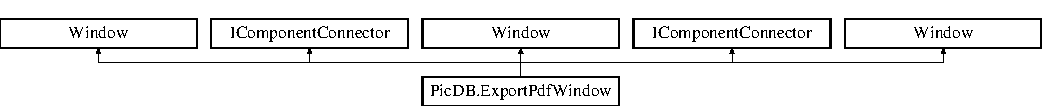
\includegraphics[height=1.417722cm]{class_pic_d_b_1_1_export_pdf_window}
\end{center}
\end{figure}
\subsection*{Public Member Functions}
\begin{DoxyCompactItemize}
\item 
\mbox{\Hypertarget{class_pic_d_b_1_1_export_pdf_window_a0fe8d98f400f446a54f83e5be855c66c}\label{class_pic_d_b_1_1_export_pdf_window_a0fe8d98f400f446a54f83e5be855c66c}} 
{\bfseries Export\+Pdf\+Window} (\mbox{\hyperlink{class_pic_d_b_1_1_view_models_1_1_main_window_view_model}{Main\+Window\+View\+Model}} controller)
\item 
void \mbox{\hyperlink{class_pic_d_b_1_1_export_pdf_window_aad2857cbab242278820d73fb64af3fb6}{Initialize\+Component}} ()
\begin{DoxyCompactList}\small\item\em Initialize\+Component \end{DoxyCompactList}\item 
void \mbox{\hyperlink{class_pic_d_b_1_1_export_pdf_window_aad2857cbab242278820d73fb64af3fb6}{Initialize\+Component}} ()
\begin{DoxyCompactList}\small\item\em Initialize\+Component \end{DoxyCompactList}\end{DoxyCompactItemize}


\subsection{Detailed Description}
Interaction logic for Export\+Pdf\+Window.\+xaml 

\mbox{\hyperlink{class_pic_d_b_1_1_export_pdf_window}{Export\+Pdf\+Window}} 

\subsection{Member Function Documentation}
\mbox{\Hypertarget{class_pic_d_b_1_1_export_pdf_window_aad2857cbab242278820d73fb64af3fb6}\label{class_pic_d_b_1_1_export_pdf_window_aad2857cbab242278820d73fb64af3fb6}} 
\index{Pic\+D\+B\+::\+Export\+Pdf\+Window@{Pic\+D\+B\+::\+Export\+Pdf\+Window}!Initialize\+Component@{Initialize\+Component}}
\index{Initialize\+Component@{Initialize\+Component}!Pic\+D\+B\+::\+Export\+Pdf\+Window@{Pic\+D\+B\+::\+Export\+Pdf\+Window}}
\subsubsection{\texorpdfstring{Initialize\+Component()}{InitializeComponent()}\hspace{0.1cm}{\footnotesize\ttfamily [1/2]}}
{\footnotesize\ttfamily void Pic\+D\+B.\+Export\+Pdf\+Window.\+Initialize\+Component (\begin{DoxyParamCaption}{ }\end{DoxyParamCaption})}



Initialize\+Component 

\mbox{\Hypertarget{class_pic_d_b_1_1_export_pdf_window_aad2857cbab242278820d73fb64af3fb6}\label{class_pic_d_b_1_1_export_pdf_window_aad2857cbab242278820d73fb64af3fb6}} 
\index{Pic\+D\+B\+::\+Export\+Pdf\+Window@{Pic\+D\+B\+::\+Export\+Pdf\+Window}!Initialize\+Component@{Initialize\+Component}}
\index{Initialize\+Component@{Initialize\+Component}!Pic\+D\+B\+::\+Export\+Pdf\+Window@{Pic\+D\+B\+::\+Export\+Pdf\+Window}}
\subsubsection{\texorpdfstring{Initialize\+Component()}{InitializeComponent()}\hspace{0.1cm}{\footnotesize\ttfamily [2/2]}}
{\footnotesize\ttfamily void Pic\+D\+B.\+Export\+Pdf\+Window.\+Initialize\+Component (\begin{DoxyParamCaption}{ }\end{DoxyParamCaption})}



Initialize\+Component 



The documentation for this class was generated from the following files\+:\begin{DoxyCompactItemize}
\item 
C\+:/\+A\+A\+A-\/\+Technikum\+\_\+\+B\+W\+I/fourth\+Semester/\+S\+W\+E2/\+S\+W\+E2-\/\+C\+S/\+Pic\+D\+B/Export\+Pdf\+Window.\+xaml.\+cs\item 
C\+:/\+A\+A\+A-\/\+Technikum\+\_\+\+B\+W\+I/fourth\+Semester/\+S\+W\+E2/\+S\+W\+E2-\/\+C\+S/\+Pic\+D\+B/obj/x86/\+Debug/Export\+Pdf\+Window.\+g.\+cs\item 
C\+:/\+A\+A\+A-\/\+Technikum\+\_\+\+B\+W\+I/fourth\+Semester/\+S\+W\+E2/\+S\+W\+E2-\/\+C\+S/\+Pic\+D\+B/obj/x86/\+Debug/Export\+Pdf\+Window.\+g.\+i.\+cs\end{DoxyCompactItemize}

\hypertarget{class_pic_d_b_1_1_models_1_1_i_p_t_c_model}{}\section{Pic\+D\+B.\+Models.\+I\+P\+T\+C\+Model Class Reference}
\label{class_pic_d_b_1_1_models_1_1_i_p_t_c_model}\index{Pic\+D\+B.\+Models.\+I\+P\+T\+C\+Model@{Pic\+D\+B.\+Models.\+I\+P\+T\+C\+Model}}


A model for I\+P\+TC information of a picture  


Inheritance diagram for Pic\+D\+B.\+Models.\+I\+P\+T\+C\+Model\+:\begin{figure}[H]
\begin{center}
\leavevmode
\includegraphics[height=2.000000cm]{class_pic_d_b_1_1_models_1_1_i_p_t_c_model}
\end{center}
\end{figure}
\subsection*{Public Member Functions}
\begin{DoxyCompactItemize}
\item 
\mbox{\Hypertarget{class_pic_d_b_1_1_models_1_1_i_p_t_c_model_a5ead69afb51c0335e36d1668be1a4ae2}\label{class_pic_d_b_1_1_models_1_1_i_p_t_c_model_a5ead69afb51c0335e36d1668be1a4ae2}} 
{\bfseries I\+P\+T\+C\+Model} (I\+I\+P\+T\+C\+View\+Model view\+Model)
\end{DoxyCompactItemize}
\subsection*{Properties}
\begin{DoxyCompactItemize}
\item 
string \mbox{\hyperlink{class_pic_d_b_1_1_models_1_1_i_p_t_c_model_a60958a1ca8c9800f6499aaddd73ac5e6}{Keywords}}\hspace{0.3cm}{\ttfamily  \mbox{[}get, set\mbox{]}}
\begin{DoxyCompactList}\small\item\em A list of keywords \end{DoxyCompactList}\item 
string \mbox{\hyperlink{class_pic_d_b_1_1_models_1_1_i_p_t_c_model_a5c73683dbe7b1c2d95057b97f1596e25}{By\+Line}}\hspace{0.3cm}{\ttfamily  \mbox{[}get, set\mbox{]}}
\begin{DoxyCompactList}\small\item\em Name of the photographer \end{DoxyCompactList}\item 
string \mbox{\hyperlink{class_pic_d_b_1_1_models_1_1_i_p_t_c_model_a74f5bbf0072f3f259d516e5b93d55813}{Copyright\+Notice}}\hspace{0.3cm}{\ttfamily  \mbox{[}get, set\mbox{]}}
\begin{DoxyCompactList}\small\item\em copyright notices \end{DoxyCompactList}\item 
string \mbox{\hyperlink{class_pic_d_b_1_1_models_1_1_i_p_t_c_model_a5294f413c85e8d93ae28471ba66083f3}{Headline}}\hspace{0.3cm}{\ttfamily  \mbox{[}get, set\mbox{]}}
\begin{DoxyCompactList}\small\item\em Headline of picture \end{DoxyCompactList}\item 
string \mbox{\hyperlink{class_pic_d_b_1_1_models_1_1_i_p_t_c_model_a7dd9a33da934151380170190496b4bf1}{Caption}}\hspace{0.3cm}{\ttfamily  \mbox{[}get, set\mbox{]}}
\begin{DoxyCompactList}\small\item\em description of picture \end{DoxyCompactList}\end{DoxyCompactItemize}


\subsection{Detailed Description}
A model for I\+P\+TC information of a picture 



\subsection{Property Documentation}
\mbox{\Hypertarget{class_pic_d_b_1_1_models_1_1_i_p_t_c_model_a5c73683dbe7b1c2d95057b97f1596e25}\label{class_pic_d_b_1_1_models_1_1_i_p_t_c_model_a5c73683dbe7b1c2d95057b97f1596e25}} 
\index{Pic\+D\+B\+::\+Models\+::\+I\+P\+T\+C\+Model@{Pic\+D\+B\+::\+Models\+::\+I\+P\+T\+C\+Model}!By\+Line@{By\+Line}}
\index{By\+Line@{By\+Line}!Pic\+D\+B\+::\+Models\+::\+I\+P\+T\+C\+Model@{Pic\+D\+B\+::\+Models\+::\+I\+P\+T\+C\+Model}}
\subsubsection{\texorpdfstring{By\+Line}{ByLine}}
{\footnotesize\ttfamily string Pic\+D\+B.\+Models.\+I\+P\+T\+C\+Model.\+By\+Line\hspace{0.3cm}{\ttfamily [get]}, {\ttfamily [set]}}



Name of the photographer 

\mbox{\Hypertarget{class_pic_d_b_1_1_models_1_1_i_p_t_c_model_a7dd9a33da934151380170190496b4bf1}\label{class_pic_d_b_1_1_models_1_1_i_p_t_c_model_a7dd9a33da934151380170190496b4bf1}} 
\index{Pic\+D\+B\+::\+Models\+::\+I\+P\+T\+C\+Model@{Pic\+D\+B\+::\+Models\+::\+I\+P\+T\+C\+Model}!Caption@{Caption}}
\index{Caption@{Caption}!Pic\+D\+B\+::\+Models\+::\+I\+P\+T\+C\+Model@{Pic\+D\+B\+::\+Models\+::\+I\+P\+T\+C\+Model}}
\subsubsection{\texorpdfstring{Caption}{Caption}}
{\footnotesize\ttfamily string Pic\+D\+B.\+Models.\+I\+P\+T\+C\+Model.\+Caption\hspace{0.3cm}{\ttfamily [get]}, {\ttfamily [set]}}



description of picture 

\mbox{\Hypertarget{class_pic_d_b_1_1_models_1_1_i_p_t_c_model_a74f5bbf0072f3f259d516e5b93d55813}\label{class_pic_d_b_1_1_models_1_1_i_p_t_c_model_a74f5bbf0072f3f259d516e5b93d55813}} 
\index{Pic\+D\+B\+::\+Models\+::\+I\+P\+T\+C\+Model@{Pic\+D\+B\+::\+Models\+::\+I\+P\+T\+C\+Model}!Copyright\+Notice@{Copyright\+Notice}}
\index{Copyright\+Notice@{Copyright\+Notice}!Pic\+D\+B\+::\+Models\+::\+I\+P\+T\+C\+Model@{Pic\+D\+B\+::\+Models\+::\+I\+P\+T\+C\+Model}}
\subsubsection{\texorpdfstring{Copyright\+Notice}{CopyrightNotice}}
{\footnotesize\ttfamily string Pic\+D\+B.\+Models.\+I\+P\+T\+C\+Model.\+Copyright\+Notice\hspace{0.3cm}{\ttfamily [get]}, {\ttfamily [set]}}



copyright notices 

\mbox{\Hypertarget{class_pic_d_b_1_1_models_1_1_i_p_t_c_model_a5294f413c85e8d93ae28471ba66083f3}\label{class_pic_d_b_1_1_models_1_1_i_p_t_c_model_a5294f413c85e8d93ae28471ba66083f3}} 
\index{Pic\+D\+B\+::\+Models\+::\+I\+P\+T\+C\+Model@{Pic\+D\+B\+::\+Models\+::\+I\+P\+T\+C\+Model}!Headline@{Headline}}
\index{Headline@{Headline}!Pic\+D\+B\+::\+Models\+::\+I\+P\+T\+C\+Model@{Pic\+D\+B\+::\+Models\+::\+I\+P\+T\+C\+Model}}
\subsubsection{\texorpdfstring{Headline}{Headline}}
{\footnotesize\ttfamily string Pic\+D\+B.\+Models.\+I\+P\+T\+C\+Model.\+Headline\hspace{0.3cm}{\ttfamily [get]}, {\ttfamily [set]}}



Headline of picture 

\mbox{\Hypertarget{class_pic_d_b_1_1_models_1_1_i_p_t_c_model_a60958a1ca8c9800f6499aaddd73ac5e6}\label{class_pic_d_b_1_1_models_1_1_i_p_t_c_model_a60958a1ca8c9800f6499aaddd73ac5e6}} 
\index{Pic\+D\+B\+::\+Models\+::\+I\+P\+T\+C\+Model@{Pic\+D\+B\+::\+Models\+::\+I\+P\+T\+C\+Model}!Keywords@{Keywords}}
\index{Keywords@{Keywords}!Pic\+D\+B\+::\+Models\+::\+I\+P\+T\+C\+Model@{Pic\+D\+B\+::\+Models\+::\+I\+P\+T\+C\+Model}}
\subsubsection{\texorpdfstring{Keywords}{Keywords}}
{\footnotesize\ttfamily string Pic\+D\+B.\+Models.\+I\+P\+T\+C\+Model.\+Keywords\hspace{0.3cm}{\ttfamily [get]}, {\ttfamily [set]}}



A list of keywords 



The documentation for this class was generated from the following file\+:\begin{DoxyCompactItemize}
\item 
C\+:/\+A\+A\+A-\/\+Technikum\+\_\+\+B\+W\+I/fourth\+Semester/\+S\+W\+E2/\+S\+W\+E2-\/\+C\+S/\+Pic\+D\+B/\+Models/I\+P\+T\+C\+Model.\+cs\end{DoxyCompactItemize}

\hypertarget{class_pic_d_b_1_1_view_models_1_1_i_p_t_c_view_model}{}\section{Pic\+D\+B.\+View\+Models.\+I\+P\+T\+C\+View\+Model Class Reference}
\label{class_pic_d_b_1_1_view_models_1_1_i_p_t_c_view_model}\index{Pic\+D\+B.\+View\+Models.\+I\+P\+T\+C\+View\+Model@{Pic\+D\+B.\+View\+Models.\+I\+P\+T\+C\+View\+Model}}


A viewmodel of I\+P\+TC information of a picture  


Inheritance diagram for Pic\+D\+B.\+View\+Models.\+I\+P\+T\+C\+View\+Model\+:\begin{figure}[H]
\begin{center}
\leavevmode
\includegraphics[height=2.000000cm]{class_pic_d_b_1_1_view_models_1_1_i_p_t_c_view_model}
\end{center}
\end{figure}
\subsection*{Public Member Functions}
\begin{DoxyCompactItemize}
\item 
\mbox{\Hypertarget{class_pic_d_b_1_1_view_models_1_1_i_p_t_c_view_model_a78d3aa2f6a067518ae5f5675433b90a9}\label{class_pic_d_b_1_1_view_models_1_1_i_p_t_c_view_model_a78d3aa2f6a067518ae5f5675433b90a9}} 
{\bfseries I\+P\+T\+C\+View\+Model} (I\+I\+P\+T\+C\+Model model)
\end{DoxyCompactItemize}
\subsection*{Public Attributes}
\begin{DoxyCompactItemize}
\item 
I\+Enumerable$<$ string $>$ \mbox{\hyperlink{class_pic_d_b_1_1_view_models_1_1_i_p_t_c_view_model_adce53c4d69fca3cb1fd53a3fabd28d0d}{Copyright\+Notices}} =$>$ \+\_\+copyright\+Notices
\begin{DoxyCompactList}\small\item\em A list of common copyright noties. e.\+g. All rights reserved, C\+C-\/\+BY, C\+C-\/\+B\+Y-\/\+SA, C\+C-\/\+B\+Y-\/\+ND, C\+C-\/\+B\+Y-\/\+NC, C\+C-\/\+B\+Y-\/\+N\+C-\/\+SA, C\+C-\/\+B\+Y-\/\+N\+C-\/\+ND \end{DoxyCompactList}\end{DoxyCompactItemize}
\subsection*{Properties}
\begin{DoxyCompactItemize}
\item 
string \mbox{\hyperlink{class_pic_d_b_1_1_view_models_1_1_i_p_t_c_view_model_a0358809f08dae5ca402fbd91f62eeef5}{Keywords}}\hspace{0.3cm}{\ttfamily  \mbox{[}get, set\mbox{]}}
\begin{DoxyCompactList}\small\item\em A list of keywords \end{DoxyCompactList}\item 
string \mbox{\hyperlink{class_pic_d_b_1_1_view_models_1_1_i_p_t_c_view_model_adeef9f73b094c9d6b313ad61585c7ea6}{By\+Line}}\hspace{0.3cm}{\ttfamily  \mbox{[}get, set\mbox{]}}
\begin{DoxyCompactList}\small\item\em Name of the photographer \end{DoxyCompactList}\item 
string \mbox{\hyperlink{class_pic_d_b_1_1_view_models_1_1_i_p_t_c_view_model_a08983c5e75d28ba6730d7cf46abb2c18}{Copyright\+Notice}}\hspace{0.3cm}{\ttfamily  \mbox{[}get, set\mbox{]}}
\begin{DoxyCompactList}\small\item\em copyright noties. \end{DoxyCompactList}\item 
string \mbox{\hyperlink{class_pic_d_b_1_1_view_models_1_1_i_p_t_c_view_model_aac14ee1d79fb32cfe75980c6e179c079}{Headline}}\hspace{0.3cm}{\ttfamily  \mbox{[}get, set\mbox{]}}
\begin{DoxyCompactList}\small\item\em Summary/\+Headline of the picture \end{DoxyCompactList}\item 
string \mbox{\hyperlink{class_pic_d_b_1_1_view_models_1_1_i_p_t_c_view_model_a8aaa4a445411478497dcfc0128172a60}{Caption}}\hspace{0.3cm}{\ttfamily  \mbox{[}get, set\mbox{]}}
\begin{DoxyCompactList}\small\item\em Caption/\+Abstract, a description of the picture \end{DoxyCompactList}\end{DoxyCompactItemize}


\subsection{Detailed Description}
A viewmodel of I\+P\+TC information of a picture 



\subsection{Member Data Documentation}
\mbox{\Hypertarget{class_pic_d_b_1_1_view_models_1_1_i_p_t_c_view_model_adce53c4d69fca3cb1fd53a3fabd28d0d}\label{class_pic_d_b_1_1_view_models_1_1_i_p_t_c_view_model_adce53c4d69fca3cb1fd53a3fabd28d0d}} 
\index{Pic\+D\+B\+::\+View\+Models\+::\+I\+P\+T\+C\+View\+Model@{Pic\+D\+B\+::\+View\+Models\+::\+I\+P\+T\+C\+View\+Model}!Copyright\+Notices@{Copyright\+Notices}}
\index{Copyright\+Notices@{Copyright\+Notices}!Pic\+D\+B\+::\+View\+Models\+::\+I\+P\+T\+C\+View\+Model@{Pic\+D\+B\+::\+View\+Models\+::\+I\+P\+T\+C\+View\+Model}}
\subsubsection{\texorpdfstring{Copyright\+Notices}{CopyrightNotices}}
{\footnotesize\ttfamily I\+Enumerable$<$string$>$ Pic\+D\+B.\+View\+Models.\+I\+P\+T\+C\+View\+Model.\+Copyright\+Notices =$>$ \+\_\+copyright\+Notices}



A list of common copyright noties. e.\+g. All rights reserved, C\+C-\/\+BY, C\+C-\/\+B\+Y-\/\+SA, C\+C-\/\+B\+Y-\/\+ND, C\+C-\/\+B\+Y-\/\+NC, C\+C-\/\+B\+Y-\/\+N\+C-\/\+SA, C\+C-\/\+B\+Y-\/\+N\+C-\/\+ND 



\subsection{Property Documentation}
\mbox{\Hypertarget{class_pic_d_b_1_1_view_models_1_1_i_p_t_c_view_model_adeef9f73b094c9d6b313ad61585c7ea6}\label{class_pic_d_b_1_1_view_models_1_1_i_p_t_c_view_model_adeef9f73b094c9d6b313ad61585c7ea6}} 
\index{Pic\+D\+B\+::\+View\+Models\+::\+I\+P\+T\+C\+View\+Model@{Pic\+D\+B\+::\+View\+Models\+::\+I\+P\+T\+C\+View\+Model}!By\+Line@{By\+Line}}
\index{By\+Line@{By\+Line}!Pic\+D\+B\+::\+View\+Models\+::\+I\+P\+T\+C\+View\+Model@{Pic\+D\+B\+::\+View\+Models\+::\+I\+P\+T\+C\+View\+Model}}
\subsubsection{\texorpdfstring{By\+Line}{ByLine}}
{\footnotesize\ttfamily string Pic\+D\+B.\+View\+Models.\+I\+P\+T\+C\+View\+Model.\+By\+Line\hspace{0.3cm}{\ttfamily [get]}, {\ttfamily [set]}}



Name of the photographer 

\mbox{\Hypertarget{class_pic_d_b_1_1_view_models_1_1_i_p_t_c_view_model_a8aaa4a445411478497dcfc0128172a60}\label{class_pic_d_b_1_1_view_models_1_1_i_p_t_c_view_model_a8aaa4a445411478497dcfc0128172a60}} 
\index{Pic\+D\+B\+::\+View\+Models\+::\+I\+P\+T\+C\+View\+Model@{Pic\+D\+B\+::\+View\+Models\+::\+I\+P\+T\+C\+View\+Model}!Caption@{Caption}}
\index{Caption@{Caption}!Pic\+D\+B\+::\+View\+Models\+::\+I\+P\+T\+C\+View\+Model@{Pic\+D\+B\+::\+View\+Models\+::\+I\+P\+T\+C\+View\+Model}}
\subsubsection{\texorpdfstring{Caption}{Caption}}
{\footnotesize\ttfamily string Pic\+D\+B.\+View\+Models.\+I\+P\+T\+C\+View\+Model.\+Caption\hspace{0.3cm}{\ttfamily [get]}, {\ttfamily [set]}}



Caption/\+Abstract, a description of the picture 

\mbox{\Hypertarget{class_pic_d_b_1_1_view_models_1_1_i_p_t_c_view_model_a08983c5e75d28ba6730d7cf46abb2c18}\label{class_pic_d_b_1_1_view_models_1_1_i_p_t_c_view_model_a08983c5e75d28ba6730d7cf46abb2c18}} 
\index{Pic\+D\+B\+::\+View\+Models\+::\+I\+P\+T\+C\+View\+Model@{Pic\+D\+B\+::\+View\+Models\+::\+I\+P\+T\+C\+View\+Model}!Copyright\+Notice@{Copyright\+Notice}}
\index{Copyright\+Notice@{Copyright\+Notice}!Pic\+D\+B\+::\+View\+Models\+::\+I\+P\+T\+C\+View\+Model@{Pic\+D\+B\+::\+View\+Models\+::\+I\+P\+T\+C\+View\+Model}}
\subsubsection{\texorpdfstring{Copyright\+Notice}{CopyrightNotice}}
{\footnotesize\ttfamily string Pic\+D\+B.\+View\+Models.\+I\+P\+T\+C\+View\+Model.\+Copyright\+Notice\hspace{0.3cm}{\ttfamily [get]}, {\ttfamily [set]}}



copyright noties. 

\mbox{\Hypertarget{class_pic_d_b_1_1_view_models_1_1_i_p_t_c_view_model_aac14ee1d79fb32cfe75980c6e179c079}\label{class_pic_d_b_1_1_view_models_1_1_i_p_t_c_view_model_aac14ee1d79fb32cfe75980c6e179c079}} 
\index{Pic\+D\+B\+::\+View\+Models\+::\+I\+P\+T\+C\+View\+Model@{Pic\+D\+B\+::\+View\+Models\+::\+I\+P\+T\+C\+View\+Model}!Headline@{Headline}}
\index{Headline@{Headline}!Pic\+D\+B\+::\+View\+Models\+::\+I\+P\+T\+C\+View\+Model@{Pic\+D\+B\+::\+View\+Models\+::\+I\+P\+T\+C\+View\+Model}}
\subsubsection{\texorpdfstring{Headline}{Headline}}
{\footnotesize\ttfamily string Pic\+D\+B.\+View\+Models.\+I\+P\+T\+C\+View\+Model.\+Headline\hspace{0.3cm}{\ttfamily [get]}, {\ttfamily [set]}}



Summary/\+Headline of the picture 

\mbox{\Hypertarget{class_pic_d_b_1_1_view_models_1_1_i_p_t_c_view_model_a0358809f08dae5ca402fbd91f62eeef5}\label{class_pic_d_b_1_1_view_models_1_1_i_p_t_c_view_model_a0358809f08dae5ca402fbd91f62eeef5}} 
\index{Pic\+D\+B\+::\+View\+Models\+::\+I\+P\+T\+C\+View\+Model@{Pic\+D\+B\+::\+View\+Models\+::\+I\+P\+T\+C\+View\+Model}!Keywords@{Keywords}}
\index{Keywords@{Keywords}!Pic\+D\+B\+::\+View\+Models\+::\+I\+P\+T\+C\+View\+Model@{Pic\+D\+B\+::\+View\+Models\+::\+I\+P\+T\+C\+View\+Model}}
\subsubsection{\texorpdfstring{Keywords}{Keywords}}
{\footnotesize\ttfamily string Pic\+D\+B.\+View\+Models.\+I\+P\+T\+C\+View\+Model.\+Keywords\hspace{0.3cm}{\ttfamily [get]}, {\ttfamily [set]}}



A list of keywords 



The documentation for this class was generated from the following file\+:\begin{DoxyCompactItemize}
\item 
C\+:/\+A\+A\+A-\/\+Technikum\+\_\+\+B\+W\+I/fourth\+Semester/\+S\+W\+E2/\+S\+W\+E2-\/\+C\+S/\+Pic\+D\+B/\+View\+Models/I\+P\+T\+C\+View\+Model.\+cs\end{DoxyCompactItemize}

\hypertarget{class_pic_d_b_1_1_main_window}{}\section{Pic\+D\+B.\+Main\+Window Class Reference}
\label{class_pic_d_b_1_1_main_window}\index{Pic\+D\+B.\+Main\+Window@{Pic\+D\+B.\+Main\+Window}}


Interaction logic for Main\+Window.\+xaml  


Inheritance diagram for Pic\+D\+B.\+Main\+Window\+:\begin{figure}[H]
\begin{center}
\leavevmode
\includegraphics[height=1.544828cm]{class_pic_d_b_1_1_main_window}
\end{center}
\end{figure}
\subsection*{Public Member Functions}
\begin{DoxyCompactItemize}
\item 
void \mbox{\hyperlink{class_pic_d_b_1_1_main_window_a5b3ff51020040626afa96b204d0e41c6}{Initialize\+Component}} ()
\begin{DoxyCompactList}\small\item\em Initialize\+Component \end{DoxyCompactList}\item 
void \mbox{\hyperlink{class_pic_d_b_1_1_main_window_a5b3ff51020040626afa96b204d0e41c6}{Initialize\+Component}} ()
\begin{DoxyCompactList}\small\item\em Initialize\+Component \end{DoxyCompactList}\end{DoxyCompactItemize}


\subsection{Detailed Description}
Interaction logic for Main\+Window.\+xaml 

\mbox{\hyperlink{class_pic_d_b_1_1_main_window}{Main\+Window}} 

\subsection{Member Function Documentation}
\mbox{\Hypertarget{class_pic_d_b_1_1_main_window_a5b3ff51020040626afa96b204d0e41c6}\label{class_pic_d_b_1_1_main_window_a5b3ff51020040626afa96b204d0e41c6}} 
\index{Pic\+D\+B\+::\+Main\+Window@{Pic\+D\+B\+::\+Main\+Window}!Initialize\+Component@{Initialize\+Component}}
\index{Initialize\+Component@{Initialize\+Component}!Pic\+D\+B\+::\+Main\+Window@{Pic\+D\+B\+::\+Main\+Window}}
\subsubsection{\texorpdfstring{Initialize\+Component()}{InitializeComponent()}\hspace{0.1cm}{\footnotesize\ttfamily [1/2]}}
{\footnotesize\ttfamily void Pic\+D\+B.\+Main\+Window.\+Initialize\+Component (\begin{DoxyParamCaption}{ }\end{DoxyParamCaption})}



Initialize\+Component 

\mbox{\Hypertarget{class_pic_d_b_1_1_main_window_a5b3ff51020040626afa96b204d0e41c6}\label{class_pic_d_b_1_1_main_window_a5b3ff51020040626afa96b204d0e41c6}} 
\index{Pic\+D\+B\+::\+Main\+Window@{Pic\+D\+B\+::\+Main\+Window}!Initialize\+Component@{Initialize\+Component}}
\index{Initialize\+Component@{Initialize\+Component}!Pic\+D\+B\+::\+Main\+Window@{Pic\+D\+B\+::\+Main\+Window}}
\subsubsection{\texorpdfstring{Initialize\+Component()}{InitializeComponent()}\hspace{0.1cm}{\footnotesize\ttfamily [2/2]}}
{\footnotesize\ttfamily void Pic\+D\+B.\+Main\+Window.\+Initialize\+Component (\begin{DoxyParamCaption}{ }\end{DoxyParamCaption})}



Initialize\+Component 



The documentation for this class was generated from the following files\+:\begin{DoxyCompactItemize}
\item 
C\+:/\+A\+A\+A-\/\+Technikum\+\_\+\+B\+W\+I/fourth\+Semester/\+S\+W\+E2/\+S\+W\+E2-\/\+C\+S/\+Pic\+D\+B/Main\+Window.\+xaml.\+cs\item 
C\+:/\+A\+A\+A-\/\+Technikum\+\_\+\+B\+W\+I/fourth\+Semester/\+S\+W\+E2/\+S\+W\+E2-\/\+C\+S/\+Pic\+D\+B/obj/x86/\+Debug/Main\+Window.\+g.\+cs\item 
C\+:/\+A\+A\+A-\/\+Technikum\+\_\+\+B\+W\+I/fourth\+Semester/\+S\+W\+E2/\+S\+W\+E2-\/\+C\+S/\+Pic\+D\+B/obj/x86/\+Debug/Main\+Window.\+g.\+i.\+cs\end{DoxyCompactItemize}

\hypertarget{class_pic_d_b_1_1_view_models_1_1_main_window_view_model}{}\section{Pic\+D\+B.\+View\+Models.\+Main\+Window\+View\+Model Class Reference}
\label{class_pic_d_b_1_1_view_models_1_1_main_window_view_model}\index{Pic\+D\+B.\+View\+Models.\+Main\+Window\+View\+Model@{Pic\+D\+B.\+View\+Models.\+Main\+Window\+View\+Model}}


Controller. Use this if changes come F\+R\+OM the UI.  


Inheritance diagram for Pic\+D\+B.\+View\+Models.\+Main\+Window\+View\+Model\+:\begin{figure}[H]
\begin{center}
\leavevmode
\includegraphics[height=3.000000cm]{class_pic_d_b_1_1_view_models_1_1_main_window_view_model}
\end{center}
\end{figure}
\subsection*{Public Member Functions}
\begin{DoxyCompactItemize}
\item 
void \mbox{\hyperlink{class_pic_d_b_1_1_view_models_1_1_main_window_view_model_aec5f805a75b05d57d6c8a057a874519e}{Save\+Current\+Picture}} ()
\begin{DoxyCompactList}\small\item\em Saves currently selected picture to DB \end{DoxyCompactList}\item 
void \mbox{\hyperlink{class_pic_d_b_1_1_view_models_1_1_main_window_view_model_ada19d2955e0f0bfc31920483a53f4850}{Save\+Camera}} (\mbox{\hyperlink{class_pic_d_b_1_1_view_models_1_1_camera_view_model}{Camera\+View\+Model}} camera)
\begin{DoxyCompactList}\small\item\em Saves new camera to DB \end{DoxyCompactList}\item 
void \mbox{\hyperlink{class_pic_d_b_1_1_view_models_1_1_main_window_view_model_a122865147968287045a9390940c1582c}{Update\+Photographer}} (\mbox{\hyperlink{class_pic_d_b_1_1_view_models_1_1_photographer_view_model}{Photographer\+View\+Model}} photographer\+View\+Model)
\begin{DoxyCompactList}\small\item\em Updates photographer \end{DoxyCompactList}\item 
void \mbox{\hyperlink{class_pic_d_b_1_1_view_models_1_1_main_window_view_model_a26618fe0f1e947caf7ab7f4ca94941f2}{Delete\+Photographer}} (int id)
\begin{DoxyCompactList}\small\item\em Deletes photographer with given ID \end{DoxyCompactList}\end{DoxyCompactItemize}
\subsection*{Properties}
\begin{DoxyCompactItemize}
\item 
I\+Picture\+View\+Model \mbox{\hyperlink{class_pic_d_b_1_1_view_models_1_1_main_window_view_model_a9c4c52c2062c53ea3cf37be5fdb0842d}{Current\+Picture}}\hspace{0.3cm}{\ttfamily  \mbox{[}get, set\mbox{]}}
\begin{DoxyCompactList}\small\item\em Currently selected picture in the UI \end{DoxyCompactList}\item 
string \mbox{\hyperlink{class_pic_d_b_1_1_view_models_1_1_main_window_view_model_a1d4dda65b12fb29886d0eab473b6912b}{Title}}\hspace{0.3cm}{\ttfamily  \mbox{[}get, set\mbox{]}}
\begin{DoxyCompactList}\small\item\em Title to be displayed in \mbox{\hyperlink{class_pic_d_b_1_1_main_window}{Main\+Window}} \end{DoxyCompactList}\item 
I\+Picture\+List\+View\+Model \mbox{\hyperlink{class_pic_d_b_1_1_view_models_1_1_main_window_view_model_aa061a2f456ed8f7817d6cc2f42726a09}{List}} = new \mbox{\hyperlink{class_pic_d_b_1_1_view_models_1_1_picture_list_view_model}{Picture\+List\+View\+Model}}()\hspace{0.3cm}{\ttfamily  \mbox{[}get, set\mbox{]}}
\begin{DoxyCompactList}\small\item\em View\+Model with a list of all Pictures \end{DoxyCompactList}\item 
I\+Search\+View\+Model \mbox{\hyperlink{class_pic_d_b_1_1_view_models_1_1_main_window_view_model_af2fd2181d3ef12acc499b32399d6cfee}{Search}} = new \mbox{\hyperlink{class_pic_d_b_1_1_view_models_1_1_search_view_model}{Search\+View\+Model}}()\hspace{0.3cm}{\ttfamily  \mbox{[}get, set\mbox{]}}
\begin{DoxyCompactList}\small\item\em Search View\+Model \end{DoxyCompactList}\item 
I\+Camera\+List\+View\+Model \mbox{\hyperlink{class_pic_d_b_1_1_view_models_1_1_main_window_view_model_a6a267de19a02911ad75396c341a2b62a}{Camera\+List}} = new \mbox{\hyperlink{class_pic_d_b_1_1_view_models_1_1_camera_list_view_model}{Camera\+List\+View\+Model}}()\hspace{0.3cm}{\ttfamily  \mbox{[}get, set\mbox{]}}
\begin{DoxyCompactList}\small\item\em View\+Model with a list of all cameras \end{DoxyCompactList}\item 
I\+Photographer\+List\+View\+Model \mbox{\hyperlink{class_pic_d_b_1_1_view_models_1_1_main_window_view_model_a6cbd934dd24539156312657313f4afed}{Photographer\+List}} = new \mbox{\hyperlink{class_pic_d_b_1_1_view_models_1_1_photographer_list_view_model}{Photographer\+List\+View\+Model}}()\hspace{0.3cm}{\ttfamily  \mbox{[}get, set\mbox{]}}
\begin{DoxyCompactList}\small\item\em View\+Model witha list of all photographers \end{DoxyCompactList}\end{DoxyCompactItemize}
\subsection*{Additional Inherited Members}


\subsection{Detailed Description}
Controller. Use this if changes come F\+R\+OM the UI. 



\subsection{Member Function Documentation}
\mbox{\Hypertarget{class_pic_d_b_1_1_view_models_1_1_main_window_view_model_a26618fe0f1e947caf7ab7f4ca94941f2}\label{class_pic_d_b_1_1_view_models_1_1_main_window_view_model_a26618fe0f1e947caf7ab7f4ca94941f2}} 
\index{Pic\+D\+B\+::\+View\+Models\+::\+Main\+Window\+View\+Model@{Pic\+D\+B\+::\+View\+Models\+::\+Main\+Window\+View\+Model}!Delete\+Photographer@{Delete\+Photographer}}
\index{Delete\+Photographer@{Delete\+Photographer}!Pic\+D\+B\+::\+View\+Models\+::\+Main\+Window\+View\+Model@{Pic\+D\+B\+::\+View\+Models\+::\+Main\+Window\+View\+Model}}
\subsubsection{\texorpdfstring{Delete\+Photographer()}{DeletePhotographer()}}
{\footnotesize\ttfamily void Pic\+D\+B.\+View\+Models.\+Main\+Window\+View\+Model.\+Delete\+Photographer (\begin{DoxyParamCaption}\item[{int}]{id }\end{DoxyParamCaption})}



Deletes photographer with given ID 


\begin{DoxyParams}{Parameters}
{\em id} & \\
\hline
\end{DoxyParams}
\mbox{\Hypertarget{class_pic_d_b_1_1_view_models_1_1_main_window_view_model_ada19d2955e0f0bfc31920483a53f4850}\label{class_pic_d_b_1_1_view_models_1_1_main_window_view_model_ada19d2955e0f0bfc31920483a53f4850}} 
\index{Pic\+D\+B\+::\+View\+Models\+::\+Main\+Window\+View\+Model@{Pic\+D\+B\+::\+View\+Models\+::\+Main\+Window\+View\+Model}!Save\+Camera@{Save\+Camera}}
\index{Save\+Camera@{Save\+Camera}!Pic\+D\+B\+::\+View\+Models\+::\+Main\+Window\+View\+Model@{Pic\+D\+B\+::\+View\+Models\+::\+Main\+Window\+View\+Model}}
\subsubsection{\texorpdfstring{Save\+Camera()}{SaveCamera()}}
{\footnotesize\ttfamily void Pic\+D\+B.\+View\+Models.\+Main\+Window\+View\+Model.\+Save\+Camera (\begin{DoxyParamCaption}\item[{\mbox{\hyperlink{class_pic_d_b_1_1_view_models_1_1_camera_view_model}{Camera\+View\+Model}}}]{camera }\end{DoxyParamCaption})}



Saves new camera to DB 


\begin{DoxyParams}{Parameters}
{\em camera} & \\
\hline
\end{DoxyParams}
\mbox{\Hypertarget{class_pic_d_b_1_1_view_models_1_1_main_window_view_model_aec5f805a75b05d57d6c8a057a874519e}\label{class_pic_d_b_1_1_view_models_1_1_main_window_view_model_aec5f805a75b05d57d6c8a057a874519e}} 
\index{Pic\+D\+B\+::\+View\+Models\+::\+Main\+Window\+View\+Model@{Pic\+D\+B\+::\+View\+Models\+::\+Main\+Window\+View\+Model}!Save\+Current\+Picture@{Save\+Current\+Picture}}
\index{Save\+Current\+Picture@{Save\+Current\+Picture}!Pic\+D\+B\+::\+View\+Models\+::\+Main\+Window\+View\+Model@{Pic\+D\+B\+::\+View\+Models\+::\+Main\+Window\+View\+Model}}
\subsubsection{\texorpdfstring{Save\+Current\+Picture()}{SaveCurrentPicture()}}
{\footnotesize\ttfamily void Pic\+D\+B.\+View\+Models.\+Main\+Window\+View\+Model.\+Save\+Current\+Picture (\begin{DoxyParamCaption}{ }\end{DoxyParamCaption})}



Saves currently selected picture to DB 

\mbox{\Hypertarget{class_pic_d_b_1_1_view_models_1_1_main_window_view_model_a122865147968287045a9390940c1582c}\label{class_pic_d_b_1_1_view_models_1_1_main_window_view_model_a122865147968287045a9390940c1582c}} 
\index{Pic\+D\+B\+::\+View\+Models\+::\+Main\+Window\+View\+Model@{Pic\+D\+B\+::\+View\+Models\+::\+Main\+Window\+View\+Model}!Update\+Photographer@{Update\+Photographer}}
\index{Update\+Photographer@{Update\+Photographer}!Pic\+D\+B\+::\+View\+Models\+::\+Main\+Window\+View\+Model@{Pic\+D\+B\+::\+View\+Models\+::\+Main\+Window\+View\+Model}}
\subsubsection{\texorpdfstring{Update\+Photographer()}{UpdatePhotographer()}}
{\footnotesize\ttfamily void Pic\+D\+B.\+View\+Models.\+Main\+Window\+View\+Model.\+Update\+Photographer (\begin{DoxyParamCaption}\item[{\mbox{\hyperlink{class_pic_d_b_1_1_view_models_1_1_photographer_view_model}{Photographer\+View\+Model}}}]{photographer\+View\+Model }\end{DoxyParamCaption})}



Updates photographer 


\begin{DoxyParams}{Parameters}
{\em photographer\+View\+Model} & \\
\hline
\end{DoxyParams}


\subsection{Property Documentation}
\mbox{\Hypertarget{class_pic_d_b_1_1_view_models_1_1_main_window_view_model_a6a267de19a02911ad75396c341a2b62a}\label{class_pic_d_b_1_1_view_models_1_1_main_window_view_model_a6a267de19a02911ad75396c341a2b62a}} 
\index{Pic\+D\+B\+::\+View\+Models\+::\+Main\+Window\+View\+Model@{Pic\+D\+B\+::\+View\+Models\+::\+Main\+Window\+View\+Model}!Camera\+List@{Camera\+List}}
\index{Camera\+List@{Camera\+List}!Pic\+D\+B\+::\+View\+Models\+::\+Main\+Window\+View\+Model@{Pic\+D\+B\+::\+View\+Models\+::\+Main\+Window\+View\+Model}}
\subsubsection{\texorpdfstring{Camera\+List}{CameraList}}
{\footnotesize\ttfamily I\+Camera\+List\+View\+Model Pic\+D\+B.\+View\+Models.\+Main\+Window\+View\+Model.\+Camera\+List = new \mbox{\hyperlink{class_pic_d_b_1_1_view_models_1_1_camera_list_view_model}{Camera\+List\+View\+Model}}()\hspace{0.3cm}{\ttfamily [get]}, {\ttfamily [set]}}



View\+Model with a list of all cameras 

\mbox{\Hypertarget{class_pic_d_b_1_1_view_models_1_1_main_window_view_model_a9c4c52c2062c53ea3cf37be5fdb0842d}\label{class_pic_d_b_1_1_view_models_1_1_main_window_view_model_a9c4c52c2062c53ea3cf37be5fdb0842d}} 
\index{Pic\+D\+B\+::\+View\+Models\+::\+Main\+Window\+View\+Model@{Pic\+D\+B\+::\+View\+Models\+::\+Main\+Window\+View\+Model}!Current\+Picture@{Current\+Picture}}
\index{Current\+Picture@{Current\+Picture}!Pic\+D\+B\+::\+View\+Models\+::\+Main\+Window\+View\+Model@{Pic\+D\+B\+::\+View\+Models\+::\+Main\+Window\+View\+Model}}
\subsubsection{\texorpdfstring{Current\+Picture}{CurrentPicture}}
{\footnotesize\ttfamily I\+Picture\+View\+Model Pic\+D\+B.\+View\+Models.\+Main\+Window\+View\+Model.\+Current\+Picture\hspace{0.3cm}{\ttfamily [get]}, {\ttfamily [set]}}



Currently selected picture in the UI 

\mbox{\Hypertarget{class_pic_d_b_1_1_view_models_1_1_main_window_view_model_aa061a2f456ed8f7817d6cc2f42726a09}\label{class_pic_d_b_1_1_view_models_1_1_main_window_view_model_aa061a2f456ed8f7817d6cc2f42726a09}} 
\index{Pic\+D\+B\+::\+View\+Models\+::\+Main\+Window\+View\+Model@{Pic\+D\+B\+::\+View\+Models\+::\+Main\+Window\+View\+Model}!List@{List}}
\index{List@{List}!Pic\+D\+B\+::\+View\+Models\+::\+Main\+Window\+View\+Model@{Pic\+D\+B\+::\+View\+Models\+::\+Main\+Window\+View\+Model}}
\subsubsection{\texorpdfstring{List}{List}}
{\footnotesize\ttfamily I\+Picture\+List\+View\+Model Pic\+D\+B.\+View\+Models.\+Main\+Window\+View\+Model.\+List = new \mbox{\hyperlink{class_pic_d_b_1_1_view_models_1_1_picture_list_view_model}{Picture\+List\+View\+Model}}()\hspace{0.3cm}{\ttfamily [get]}, {\ttfamily [set]}}



View\+Model with a list of all Pictures 

\mbox{\Hypertarget{class_pic_d_b_1_1_view_models_1_1_main_window_view_model_a6cbd934dd24539156312657313f4afed}\label{class_pic_d_b_1_1_view_models_1_1_main_window_view_model_a6cbd934dd24539156312657313f4afed}} 
\index{Pic\+D\+B\+::\+View\+Models\+::\+Main\+Window\+View\+Model@{Pic\+D\+B\+::\+View\+Models\+::\+Main\+Window\+View\+Model}!Photographer\+List@{Photographer\+List}}
\index{Photographer\+List@{Photographer\+List}!Pic\+D\+B\+::\+View\+Models\+::\+Main\+Window\+View\+Model@{Pic\+D\+B\+::\+View\+Models\+::\+Main\+Window\+View\+Model}}
\subsubsection{\texorpdfstring{Photographer\+List}{PhotographerList}}
{\footnotesize\ttfamily I\+Photographer\+List\+View\+Model Pic\+D\+B.\+View\+Models.\+Main\+Window\+View\+Model.\+Photographer\+List = new \mbox{\hyperlink{class_pic_d_b_1_1_view_models_1_1_photographer_list_view_model}{Photographer\+List\+View\+Model}}()\hspace{0.3cm}{\ttfamily [get]}, {\ttfamily [set]}}



View\+Model witha list of all photographers 

\mbox{\Hypertarget{class_pic_d_b_1_1_view_models_1_1_main_window_view_model_af2fd2181d3ef12acc499b32399d6cfee}\label{class_pic_d_b_1_1_view_models_1_1_main_window_view_model_af2fd2181d3ef12acc499b32399d6cfee}} 
\index{Pic\+D\+B\+::\+View\+Models\+::\+Main\+Window\+View\+Model@{Pic\+D\+B\+::\+View\+Models\+::\+Main\+Window\+View\+Model}!Search@{Search}}
\index{Search@{Search}!Pic\+D\+B\+::\+View\+Models\+::\+Main\+Window\+View\+Model@{Pic\+D\+B\+::\+View\+Models\+::\+Main\+Window\+View\+Model}}
\subsubsection{\texorpdfstring{Search}{Search}}
{\footnotesize\ttfamily I\+Search\+View\+Model Pic\+D\+B.\+View\+Models.\+Main\+Window\+View\+Model.\+Search = new \mbox{\hyperlink{class_pic_d_b_1_1_view_models_1_1_search_view_model}{Search\+View\+Model}}()\hspace{0.3cm}{\ttfamily [get]}, {\ttfamily [set]}}



Search View\+Model 

\mbox{\Hypertarget{class_pic_d_b_1_1_view_models_1_1_main_window_view_model_a1d4dda65b12fb29886d0eab473b6912b}\label{class_pic_d_b_1_1_view_models_1_1_main_window_view_model_a1d4dda65b12fb29886d0eab473b6912b}} 
\index{Pic\+D\+B\+::\+View\+Models\+::\+Main\+Window\+View\+Model@{Pic\+D\+B\+::\+View\+Models\+::\+Main\+Window\+View\+Model}!Title@{Title}}
\index{Title@{Title}!Pic\+D\+B\+::\+View\+Models\+::\+Main\+Window\+View\+Model@{Pic\+D\+B\+::\+View\+Models\+::\+Main\+Window\+View\+Model}}
\subsubsection{\texorpdfstring{Title}{Title}}
{\footnotesize\ttfamily string Pic\+D\+B.\+View\+Models.\+Main\+Window\+View\+Model.\+Title\hspace{0.3cm}{\ttfamily [get]}, {\ttfamily [set]}}



Title to be displayed in \mbox{\hyperlink{class_pic_d_b_1_1_main_window}{Main\+Window}} 



The documentation for this class was generated from the following file\+:\begin{DoxyCompactItemize}
\item 
C\+:/\+A\+A\+A-\/\+Technikum\+\_\+\+B\+W\+I/fourth\+Semester/\+S\+W\+E2/\+S\+W\+E2-\/\+C\+S/\+Pic\+D\+B/\+View\+Models/Main\+Window\+View\+Model.\+cs\end{DoxyCompactItemize}

\hypertarget{class_pic_d_b_1_1_mocks_1_1_mock_business_layer}{}\section{Pic\+D\+B.\+Mocks.\+Mock\+Business\+Layer Class Reference}
\label{class_pic_d_b_1_1_mocks_1_1_mock_business_layer}\index{Pic\+D\+B.\+Mocks.\+Mock\+Business\+Layer@{Pic\+D\+B.\+Mocks.\+Mock\+Business\+Layer}}
Inheritance diagram for Pic\+D\+B.\+Mocks.\+Mock\+Business\+Layer\+:\begin{figure}[H]
\begin{center}
\leavevmode
\includegraphics[height=2.000000cm]{class_pic_d_b_1_1_mocks_1_1_mock_business_layer}
\end{center}
\end{figure}
\subsection*{Public Member Functions}
\begin{DoxyCompactItemize}
\item 
\mbox{\Hypertarget{class_pic_d_b_1_1_mocks_1_1_mock_business_layer_a80f17c8df1c9bdc761ab58a2aec8c641}\label{class_pic_d_b_1_1_mocks_1_1_mock_business_layer_a80f17c8df1c9bdc761ab58a2aec8c641}} 
{\bfseries Mock\+Business\+Layer} (string path)
\item 
\mbox{\Hypertarget{class_pic_d_b_1_1_mocks_1_1_mock_business_layer_afb4190c5b143c272e58da9b8aed944fd}\label{class_pic_d_b_1_1_mocks_1_1_mock_business_layer_afb4190c5b143c272e58da9b8aed944fd}} 
void {\bfseries Delete\+Photographer} (int ID)
\item 
\mbox{\Hypertarget{class_pic_d_b_1_1_mocks_1_1_mock_business_layer_a5132fb3d244b56bac77a588807db505b}\label{class_pic_d_b_1_1_mocks_1_1_mock_business_layer_a5132fb3d244b56bac77a588807db505b}} 
void {\bfseries Delete\+Picture} (int ID)
\item 
\mbox{\Hypertarget{class_pic_d_b_1_1_mocks_1_1_mock_business_layer_a5a9a8aa15656dc27ab65475a813d1d39}\label{class_pic_d_b_1_1_mocks_1_1_mock_business_layer_a5a9a8aa15656dc27ab65475a813d1d39}} 
I\+E\+X\+I\+F\+Model {\bfseries Extract\+E\+X\+IF} (string filename)
\item 
\mbox{\Hypertarget{class_pic_d_b_1_1_mocks_1_1_mock_business_layer_ae1d2b1f9e9407d2f98ad27f36b5ddedf}\label{class_pic_d_b_1_1_mocks_1_1_mock_business_layer_ae1d2b1f9e9407d2f98ad27f36b5ddedf}} 
I\+I\+P\+T\+C\+Model {\bfseries Extract\+I\+P\+TC} (string filename)
\item 
\mbox{\Hypertarget{class_pic_d_b_1_1_mocks_1_1_mock_business_layer_aa0a2c6d0f0ed15709ec4d8a25342ef8e}\label{class_pic_d_b_1_1_mocks_1_1_mock_business_layer_aa0a2c6d0f0ed15709ec4d8a25342ef8e}} 
I\+Camera\+Model {\bfseries Get\+Camera} (int ID)
\item 
\mbox{\Hypertarget{class_pic_d_b_1_1_mocks_1_1_mock_business_layer_acbdfbe27cbc52fe8d5356f4a48ea4225}\label{class_pic_d_b_1_1_mocks_1_1_mock_business_layer_acbdfbe27cbc52fe8d5356f4a48ea4225}} 
I\+Enumerable$<$ I\+Camera\+Model $>$ {\bfseries Get\+Cameras} ()
\item 
\mbox{\Hypertarget{class_pic_d_b_1_1_mocks_1_1_mock_business_layer_a9dc10d5df91337dd2f8e05ac65b70017}\label{class_pic_d_b_1_1_mocks_1_1_mock_business_layer_a9dc10d5df91337dd2f8e05ac65b70017}} 
I\+Photographer\+Model {\bfseries Get\+Photographer} (int ID)
\item 
\mbox{\Hypertarget{class_pic_d_b_1_1_mocks_1_1_mock_business_layer_af475b2eeb81f1cc0bfbd23fb58dfe118}\label{class_pic_d_b_1_1_mocks_1_1_mock_business_layer_af475b2eeb81f1cc0bfbd23fb58dfe118}} 
I\+Enumerable$<$ I\+Photographer\+Model $>$ {\bfseries Get\+Photographers} ()
\item 
\mbox{\Hypertarget{class_pic_d_b_1_1_mocks_1_1_mock_business_layer_adf79d8b71bcd31bd4c2215a7a68d0bb3}\label{class_pic_d_b_1_1_mocks_1_1_mock_business_layer_adf79d8b71bcd31bd4c2215a7a68d0bb3}} 
I\+Picture\+Model {\bfseries Get\+Picture} (int ID)
\item 
\mbox{\Hypertarget{class_pic_d_b_1_1_mocks_1_1_mock_business_layer_a052290b06e800604e6c464194883cd86}\label{class_pic_d_b_1_1_mocks_1_1_mock_business_layer_a052290b06e800604e6c464194883cd86}} 
I\+Enumerable$<$ I\+Picture\+Model $>$ {\bfseries Get\+Pictures} ()
\item 
\mbox{\Hypertarget{class_pic_d_b_1_1_mocks_1_1_mock_business_layer_a874b65f478c8278fa4354f0584949e95}\label{class_pic_d_b_1_1_mocks_1_1_mock_business_layer_a874b65f478c8278fa4354f0584949e95}} 
I\+Enumerable$<$ I\+Picture\+Model $>$ {\bfseries Get\+Pictures} (string name\+Part, I\+Photographer\+Model photographer\+Parts, I\+I\+P\+T\+C\+Model iptc\+Parts, I\+E\+X\+I\+F\+Model exif\+Parts)
\item 
\mbox{\Hypertarget{class_pic_d_b_1_1_mocks_1_1_mock_business_layer_a8168b332927e3557ce17b6cbd75869f1}\label{class_pic_d_b_1_1_mocks_1_1_mock_business_layer_a8168b332927e3557ce17b6cbd75869f1}} 
void {\bfseries Save} (I\+Picture\+Model picture)
\item 
\mbox{\Hypertarget{class_pic_d_b_1_1_mocks_1_1_mock_business_layer_a9bdf6b16cb1016fa217c1f4576d56a5d}\label{class_pic_d_b_1_1_mocks_1_1_mock_business_layer_a9bdf6b16cb1016fa217c1f4576d56a5d}} 
void {\bfseries Save} (I\+Photographer\+Model photographer)
\item 
\mbox{\Hypertarget{class_pic_d_b_1_1_mocks_1_1_mock_business_layer_a30a2c94a9bed95c115b8e8a394a99ad2}\label{class_pic_d_b_1_1_mocks_1_1_mock_business_layer_a30a2c94a9bed95c115b8e8a394a99ad2}} 
void {\bfseries Sync} ()
\item 
\mbox{\Hypertarget{class_pic_d_b_1_1_mocks_1_1_mock_business_layer_a1ac0ed401d7c32ec58e92dd3a91c7387}\label{class_pic_d_b_1_1_mocks_1_1_mock_business_layer_a1ac0ed401d7c32ec58e92dd3a91c7387}} 
void {\bfseries Write\+I\+P\+TC} (string filename, I\+I\+P\+T\+C\+Model iptc)
\end{DoxyCompactItemize}


The documentation for this class was generated from the following file\+:\begin{DoxyCompactItemize}
\item 
C\+:/\+A\+A\+A-\/\+Technikum\+\_\+\+B\+W\+I/fourth\+Semester/\+S\+W\+E2/\+S\+W\+E2-\/\+C\+S/\+Pic\+D\+B/\+Mocks/Mock\+Business\+Layer.\+cs\end{DoxyCompactItemize}

\hypertarget{class_pic_d_b_1_1_mocks_1_1_mock_data_access_layer}{}\section{Pic\+D\+B.\+Mocks.\+Mock\+Data\+Access\+Layer Class Reference}
\label{class_pic_d_b_1_1_mocks_1_1_mock_data_access_layer}\index{Pic\+D\+B.\+Mocks.\+Mock\+Data\+Access\+Layer@{Pic\+D\+B.\+Mocks.\+Mock\+Data\+Access\+Layer}}
Inheritance diagram for Pic\+D\+B.\+Mocks.\+Mock\+Data\+Access\+Layer\+:\begin{figure}[H]
\begin{center}
\leavevmode
\includegraphics[height=2.000000cm]{class_pic_d_b_1_1_mocks_1_1_mock_data_access_layer}
\end{center}
\end{figure}
\subsection*{Public Member Functions}
\begin{DoxyCompactItemize}
\item 
\mbox{\Hypertarget{class_pic_d_b_1_1_mocks_1_1_mock_data_access_layer_a98c6893cae59bb72b799129776712ebf}\label{class_pic_d_b_1_1_mocks_1_1_mock_data_access_layer_a98c6893cae59bb72b799129776712ebf}} 
void {\bfseries Delete\+Photographer} (int ID)
\item 
\mbox{\Hypertarget{class_pic_d_b_1_1_mocks_1_1_mock_data_access_layer_a64df961a433f1d99870e22cfb132eee0}\label{class_pic_d_b_1_1_mocks_1_1_mock_data_access_layer_a64df961a433f1d99870e22cfb132eee0}} 
void {\bfseries Delete\+Picture} (int ID)
\item 
\mbox{\Hypertarget{class_pic_d_b_1_1_mocks_1_1_mock_data_access_layer_ad97ea95a78c4ee68323665763da91007}\label{class_pic_d_b_1_1_mocks_1_1_mock_data_access_layer_ad97ea95a78c4ee68323665763da91007}} 
I\+Camera\+Model {\bfseries Get\+Camera} (int ID)
\item 
\mbox{\Hypertarget{class_pic_d_b_1_1_mocks_1_1_mock_data_access_layer_ad996ee27f2b414ce2015c39d5aecbdde}\label{class_pic_d_b_1_1_mocks_1_1_mock_data_access_layer_ad996ee27f2b414ce2015c39d5aecbdde}} 
I\+Enumerable$<$ I\+Camera\+Model $>$ {\bfseries Get\+Cameras} ()
\item 
\mbox{\Hypertarget{class_pic_d_b_1_1_mocks_1_1_mock_data_access_layer_a2f2f205771b7c8153e57320b00c4105d}\label{class_pic_d_b_1_1_mocks_1_1_mock_data_access_layer_a2f2f205771b7c8153e57320b00c4105d}} 
I\+Photographer\+Model {\bfseries Get\+Photographer} (int ID)
\item 
\mbox{\Hypertarget{class_pic_d_b_1_1_mocks_1_1_mock_data_access_layer_a86c530e162fb78a651f8b1243058f00c}\label{class_pic_d_b_1_1_mocks_1_1_mock_data_access_layer_a86c530e162fb78a651f8b1243058f00c}} 
I\+Enumerable$<$ I\+Photographer\+Model $>$ {\bfseries Get\+Photographers} ()
\item 
\mbox{\Hypertarget{class_pic_d_b_1_1_mocks_1_1_mock_data_access_layer_a39edd00df7e3579ded2592d0f1d8e399}\label{class_pic_d_b_1_1_mocks_1_1_mock_data_access_layer_a39edd00df7e3579ded2592d0f1d8e399}} 
I\+Picture\+Model {\bfseries Get\+Picture} (int ID)
\item 
\mbox{\Hypertarget{class_pic_d_b_1_1_mocks_1_1_mock_data_access_layer_aee45af16f1f9c40f00cce89befae2148}\label{class_pic_d_b_1_1_mocks_1_1_mock_data_access_layer_aee45af16f1f9c40f00cce89befae2148}} 
I\+Enumerable$<$ I\+Picture\+Model $>$ {\bfseries Get\+Pictures} (string name\+Part, I\+Photographer\+Model photographer\+Parts, I\+I\+P\+T\+C\+Model iptc\+Parts, I\+E\+X\+I\+F\+Model exif\+Parts)
\item 
\mbox{\Hypertarget{class_pic_d_b_1_1_mocks_1_1_mock_data_access_layer_ae31343b2301b4f7056a77c6514703fff}\label{class_pic_d_b_1_1_mocks_1_1_mock_data_access_layer_ae31343b2301b4f7056a77c6514703fff}} 
void {\bfseries Save} (I\+Picture\+Model picture)
\item 
\mbox{\Hypertarget{class_pic_d_b_1_1_mocks_1_1_mock_data_access_layer_ae024d7c16c980db4f0ef8a73ab632663}\label{class_pic_d_b_1_1_mocks_1_1_mock_data_access_layer_ae024d7c16c980db4f0ef8a73ab632663}} 
void {\bfseries Save} (I\+Photographer\+Model photographer)
\end{DoxyCompactItemize}


The documentation for this class was generated from the following file\+:\begin{DoxyCompactItemize}
\item 
C\+:/\+A\+A\+A-\/\+Technikum\+\_\+\+B\+W\+I/fourth\+Semester/\+S\+W\+E2/\+S\+W\+E2-\/\+C\+S/\+Pic\+D\+B/\+Mocks/Mock\+Data\+Access\+Layer.\+cs\end{DoxyCompactItemize}

\hypertarget{class_pic_d_b_1_1utils_1_1_pdf_report}{}\section{Pic\+D\+B.\+utils.\+Pdf\+Report Class Reference}
\label{class_pic_d_b_1_1utils_1_1_pdf_report}\index{Pic\+D\+B.\+utils.\+Pdf\+Report@{Pic\+D\+B.\+utils.\+Pdf\+Report}}


Use this to create reports as P\+DF file  


\subsection*{Public Member Functions}
\begin{DoxyCompactItemize}
\item 
void \mbox{\hyperlink{class_pic_d_b_1_1utils_1_1_pdf_report_aa7e712385da33614ab9fd81f841d9964}{Create\+Report}} (string tags)
\begin{DoxyCompactList}\small\item\em Creates a report of all tags \end{DoxyCompactList}\item 
void \mbox{\hyperlink{class_pic_d_b_1_1utils_1_1_pdf_report_aa4a4b1df10c17c5ad56028419f37d389}{Create\+Report}} (I\+Picture\+View\+Model picture)
\begin{DoxyCompactList}\small\item\em Creates a report of a single picture. \end{DoxyCompactList}\end{DoxyCompactItemize}


\subsection{Detailed Description}
Use this to create reports as P\+DF file 



\subsection{Member Function Documentation}
\mbox{\Hypertarget{class_pic_d_b_1_1utils_1_1_pdf_report_aa7e712385da33614ab9fd81f841d9964}\label{class_pic_d_b_1_1utils_1_1_pdf_report_aa7e712385da33614ab9fd81f841d9964}} 
\index{Pic\+D\+B\+::utils\+::\+Pdf\+Report@{Pic\+D\+B\+::utils\+::\+Pdf\+Report}!Create\+Report@{Create\+Report}}
\index{Create\+Report@{Create\+Report}!Pic\+D\+B\+::utils\+::\+Pdf\+Report@{Pic\+D\+B\+::utils\+::\+Pdf\+Report}}
\subsubsection{\texorpdfstring{Create\+Report()}{CreateReport()}\hspace{0.1cm}{\footnotesize\ttfamily [1/2]}}
{\footnotesize\ttfamily void Pic\+D\+B.\+utils.\+Pdf\+Report.\+Create\+Report (\begin{DoxyParamCaption}\item[{string}]{tags }\end{DoxyParamCaption})}



Creates a report of all tags 


\begin{DoxyParams}{Parameters}
{\em tags} & \\
\hline
\end{DoxyParams}
\mbox{\Hypertarget{class_pic_d_b_1_1utils_1_1_pdf_report_aa4a4b1df10c17c5ad56028419f37d389}\label{class_pic_d_b_1_1utils_1_1_pdf_report_aa4a4b1df10c17c5ad56028419f37d389}} 
\index{Pic\+D\+B\+::utils\+::\+Pdf\+Report@{Pic\+D\+B\+::utils\+::\+Pdf\+Report}!Create\+Report@{Create\+Report}}
\index{Create\+Report@{Create\+Report}!Pic\+D\+B\+::utils\+::\+Pdf\+Report@{Pic\+D\+B\+::utils\+::\+Pdf\+Report}}
\subsubsection{\texorpdfstring{Create\+Report()}{CreateReport()}\hspace{0.1cm}{\footnotesize\ttfamily [2/2]}}
{\footnotesize\ttfamily void Pic\+D\+B.\+utils.\+Pdf\+Report.\+Create\+Report (\begin{DoxyParamCaption}\item[{I\+Picture\+View\+Model}]{picture }\end{DoxyParamCaption})}



Creates a report of a single picture. 


\begin{DoxyParams}{Parameters}
{\em picture} & \\
\hline
\end{DoxyParams}


The documentation for this class was generated from the following file\+:\begin{DoxyCompactItemize}
\item 
C\+:/\+A\+A\+A-\/\+Technikum\+\_\+\+B\+W\+I/fourth\+Semester/\+S\+W\+E2/\+S\+W\+E2-\/\+C\+S/\+Pic\+D\+B/utils/Pdf\+Report.\+cs\end{DoxyCompactItemize}

\hypertarget{class_pic_d_b_1_1_photographer_add_window}{}\section{Pic\+D\+B.\+Photographer\+Add\+Window Class Reference}
\label{class_pic_d_b_1_1_photographer_add_window}\index{Pic\+D\+B.\+Photographer\+Add\+Window@{Pic\+D\+B.\+Photographer\+Add\+Window}}


\mbox{\hyperlink{class_pic_d_b_1_1_photographer_add_window}{Photographer\+Add\+Window}}  


Inheritance diagram for Pic\+D\+B.\+Photographer\+Add\+Window\+:\begin{figure}[H]
\begin{center}
\leavevmode
\includegraphics[height=1.103448cm]{class_pic_d_b_1_1_photographer_add_window}
\end{center}
\end{figure}
\subsection*{Public Member Functions}
\begin{DoxyCompactItemize}
\item 
void \mbox{\hyperlink{class_pic_d_b_1_1_photographer_add_window_aec66b53da5fcb2256a53b1c51144fcbe}{Initialize\+Component}} ()
\begin{DoxyCompactList}\small\item\em Initialize\+Component \end{DoxyCompactList}\item 
void \mbox{\hyperlink{class_pic_d_b_1_1_photographer_add_window_aec66b53da5fcb2256a53b1c51144fcbe}{Initialize\+Component}} ()
\begin{DoxyCompactList}\small\item\em Initialize\+Component \end{DoxyCompactList}\item 
\mbox{\Hypertarget{class_pic_d_b_1_1_photographer_add_window_aba19418c2227fb9383e02bf10123a4c2}\label{class_pic_d_b_1_1_photographer_add_window_aba19418c2227fb9383e02bf10123a4c2}} 
{\bfseries Photographer\+Add\+Window} (\mbox{\hyperlink{class_pic_d_b_1_1_view_models_1_1_main_window_view_model}{Main\+Window\+View\+Model}} controller)
\end{DoxyCompactItemize}


\subsection{Detailed Description}
\mbox{\hyperlink{class_pic_d_b_1_1_photographer_add_window}{Photographer\+Add\+Window}} 

Interaction logic for Photographer\+Add\+Window.\+xaml 

\subsection{Member Function Documentation}
\mbox{\Hypertarget{class_pic_d_b_1_1_photographer_add_window_aec66b53da5fcb2256a53b1c51144fcbe}\label{class_pic_d_b_1_1_photographer_add_window_aec66b53da5fcb2256a53b1c51144fcbe}} 
\index{Pic\+D\+B\+::\+Photographer\+Add\+Window@{Pic\+D\+B\+::\+Photographer\+Add\+Window}!Initialize\+Component@{Initialize\+Component}}
\index{Initialize\+Component@{Initialize\+Component}!Pic\+D\+B\+::\+Photographer\+Add\+Window@{Pic\+D\+B\+::\+Photographer\+Add\+Window}}
\subsubsection{\texorpdfstring{Initialize\+Component()}{InitializeComponent()}\hspace{0.1cm}{\footnotesize\ttfamily [1/2]}}
{\footnotesize\ttfamily void Pic\+D\+B.\+Photographer\+Add\+Window.\+Initialize\+Component (\begin{DoxyParamCaption}{ }\end{DoxyParamCaption})}



Initialize\+Component 

\mbox{\Hypertarget{class_pic_d_b_1_1_photographer_add_window_aec66b53da5fcb2256a53b1c51144fcbe}\label{class_pic_d_b_1_1_photographer_add_window_aec66b53da5fcb2256a53b1c51144fcbe}} 
\index{Pic\+D\+B\+::\+Photographer\+Add\+Window@{Pic\+D\+B\+::\+Photographer\+Add\+Window}!Initialize\+Component@{Initialize\+Component}}
\index{Initialize\+Component@{Initialize\+Component}!Pic\+D\+B\+::\+Photographer\+Add\+Window@{Pic\+D\+B\+::\+Photographer\+Add\+Window}}
\subsubsection{\texorpdfstring{Initialize\+Component()}{InitializeComponent()}\hspace{0.1cm}{\footnotesize\ttfamily [2/2]}}
{\footnotesize\ttfamily void Pic\+D\+B.\+Photographer\+Add\+Window.\+Initialize\+Component (\begin{DoxyParamCaption}{ }\end{DoxyParamCaption})}



Initialize\+Component 



The documentation for this class was generated from the following files\+:\begin{DoxyCompactItemize}
\item 
C\+:/\+A\+A\+A-\/\+Technikum\+\_\+\+B\+W\+I/fourth\+Semester/\+S\+W\+E2/\+S\+W\+E2-\/\+C\+S/\+Pic\+D\+B/obj/x86/\+Debug/Photographer\+Add\+Window.\+g.\+cs\item 
C\+:/\+A\+A\+A-\/\+Technikum\+\_\+\+B\+W\+I/fourth\+Semester/\+S\+W\+E2/\+S\+W\+E2-\/\+C\+S/\+Pic\+D\+B/obj/x86/\+Debug/Photographer\+Add\+Window.\+g.\+i.\+cs\item 
C\+:/\+A\+A\+A-\/\+Technikum\+\_\+\+B\+W\+I/fourth\+Semester/\+S\+W\+E2/\+S\+W\+E2-\/\+C\+S/\+Pic\+D\+B/Photographer\+Add\+Window.\+xaml.\+cs\end{DoxyCompactItemize}

\hypertarget{class_pic_d_b_1_1_view_models_1_1_photographer_list_view_model}{}\section{Pic\+D\+B.\+View\+Models.\+Photographer\+List\+View\+Model Class Reference}
\label{class_pic_d_b_1_1_view_models_1_1_photographer_list_view_model}\index{Pic\+D\+B.\+View\+Models.\+Photographer\+List\+View\+Model@{Pic\+D\+B.\+View\+Models.\+Photographer\+List\+View\+Model}}


View\+Model with a list of all photographers  


Inheritance diagram for Pic\+D\+B.\+View\+Models.\+Photographer\+List\+View\+Model\+:\begin{figure}[H]
\begin{center}
\leavevmode
\includegraphics[height=2.886598cm]{class_pic_d_b_1_1_view_models_1_1_photographer_list_view_model}
\end{center}
\end{figure}
\subsection*{Public Member Functions}
\begin{DoxyCompactItemize}
\item 
void \mbox{\hyperlink{class_pic_d_b_1_1_view_models_1_1_photographer_list_view_model_aabaf179c4aa8ae8146a33eca6227c2f5}{Synchronize\+Photographers}} ()
\begin{DoxyCompactList}\small\item\em Synchronizes photographerlist \end{DoxyCompactList}\end{DoxyCompactItemize}
\subsection*{Properties}
\begin{DoxyCompactItemize}
\item 
I\+Enumerable$<$ I\+Photographer\+View\+Model $>$ \mbox{\hyperlink{class_pic_d_b_1_1_view_models_1_1_photographer_list_view_model_a36cb7ad6f5651e2dde70dc3e9c136808}{List}}\hspace{0.3cm}{\ttfamily  \mbox{[}get\mbox{]}}
\begin{DoxyCompactList}\small\item\em List of all Photographer\+View\+Models \end{DoxyCompactList}\item 
I\+Photographer\+View\+Model \mbox{\hyperlink{class_pic_d_b_1_1_view_models_1_1_photographer_list_view_model_a0d1b8d5640a19a39e294f5a770ee57bf}{Current\+Photographer}}\hspace{0.3cm}{\ttfamily  \mbox{[}get, set\mbox{]}}
\begin{DoxyCompactList}\small\item\em The currently selected \mbox{\hyperlink{class_pic_d_b_1_1_view_models_1_1_photographer_view_model}{Photographer\+View\+Model}} \end{DoxyCompactList}\end{DoxyCompactItemize}
\subsection*{Additional Inherited Members}


\subsection{Detailed Description}
View\+Model with a list of all photographers 



\subsection{Member Function Documentation}
\mbox{\Hypertarget{class_pic_d_b_1_1_view_models_1_1_photographer_list_view_model_aabaf179c4aa8ae8146a33eca6227c2f5}\label{class_pic_d_b_1_1_view_models_1_1_photographer_list_view_model_aabaf179c4aa8ae8146a33eca6227c2f5}} 
\index{Pic\+D\+B\+::\+View\+Models\+::\+Photographer\+List\+View\+Model@{Pic\+D\+B\+::\+View\+Models\+::\+Photographer\+List\+View\+Model}!Synchronize\+Photographers@{Synchronize\+Photographers}}
\index{Synchronize\+Photographers@{Synchronize\+Photographers}!Pic\+D\+B\+::\+View\+Models\+::\+Photographer\+List\+View\+Model@{Pic\+D\+B\+::\+View\+Models\+::\+Photographer\+List\+View\+Model}}
\subsubsection{\texorpdfstring{Synchronize\+Photographers()}{SynchronizePhotographers()}}
{\footnotesize\ttfamily void Pic\+D\+B.\+View\+Models.\+Photographer\+List\+View\+Model.\+Synchronize\+Photographers (\begin{DoxyParamCaption}{ }\end{DoxyParamCaption})}



Synchronizes photographerlist 



\subsection{Property Documentation}
\mbox{\Hypertarget{class_pic_d_b_1_1_view_models_1_1_photographer_list_view_model_a0d1b8d5640a19a39e294f5a770ee57bf}\label{class_pic_d_b_1_1_view_models_1_1_photographer_list_view_model_a0d1b8d5640a19a39e294f5a770ee57bf}} 
\index{Pic\+D\+B\+::\+View\+Models\+::\+Photographer\+List\+View\+Model@{Pic\+D\+B\+::\+View\+Models\+::\+Photographer\+List\+View\+Model}!Current\+Photographer@{Current\+Photographer}}
\index{Current\+Photographer@{Current\+Photographer}!Pic\+D\+B\+::\+View\+Models\+::\+Photographer\+List\+View\+Model@{Pic\+D\+B\+::\+View\+Models\+::\+Photographer\+List\+View\+Model}}
\subsubsection{\texorpdfstring{Current\+Photographer}{CurrentPhotographer}}
{\footnotesize\ttfamily I\+Photographer\+View\+Model Pic\+D\+B.\+View\+Models.\+Photographer\+List\+View\+Model.\+Current\+Photographer\hspace{0.3cm}{\ttfamily [get]}, {\ttfamily [set]}}



The currently selected \mbox{\hyperlink{class_pic_d_b_1_1_view_models_1_1_photographer_view_model}{Photographer\+View\+Model}} 

\mbox{\Hypertarget{class_pic_d_b_1_1_view_models_1_1_photographer_list_view_model_a36cb7ad6f5651e2dde70dc3e9c136808}\label{class_pic_d_b_1_1_view_models_1_1_photographer_list_view_model_a36cb7ad6f5651e2dde70dc3e9c136808}} 
\index{Pic\+D\+B\+::\+View\+Models\+::\+Photographer\+List\+View\+Model@{Pic\+D\+B\+::\+View\+Models\+::\+Photographer\+List\+View\+Model}!List@{List}}
\index{List@{List}!Pic\+D\+B\+::\+View\+Models\+::\+Photographer\+List\+View\+Model@{Pic\+D\+B\+::\+View\+Models\+::\+Photographer\+List\+View\+Model}}
\subsubsection{\texorpdfstring{List}{List}}
{\footnotesize\ttfamily I\+Enumerable$<$I\+Photographer\+View\+Model$>$ Pic\+D\+B.\+View\+Models.\+Photographer\+List\+View\+Model.\+List\hspace{0.3cm}{\ttfamily [get]}}



List of all Photographer\+View\+Models 



The documentation for this class was generated from the following file\+:\begin{DoxyCompactItemize}
\item 
C\+:/\+A\+A\+A-\/\+Technikum\+\_\+\+B\+W\+I/fourth\+Semester/\+S\+W\+E2/\+S\+W\+E2-\/\+C\+S/\+Pic\+D\+B/\+View\+Models/Photographer\+List\+View\+Model.\+cs\end{DoxyCompactItemize}

\hypertarget{class_pic_d_b_1_1_models_1_1_photographer_model}{}\section{Pic\+D\+B.\+Models.\+Photographer\+Model Class Reference}
\label{class_pic_d_b_1_1_models_1_1_photographer_model}\index{Pic\+D\+B.\+Models.\+Photographer\+Model@{Pic\+D\+B.\+Models.\+Photographer\+Model}}


A model of a photographer  


Inheritance diagram for Pic\+D\+B.\+Models.\+Photographer\+Model\+:\begin{figure}[H]
\begin{center}
\leavevmode
\includegraphics[height=2.000000cm]{class_pic_d_b_1_1_models_1_1_photographer_model}
\end{center}
\end{figure}
\subsection*{Public Member Functions}
\begin{DoxyCompactItemize}
\item 
\mbox{\Hypertarget{class_pic_d_b_1_1_models_1_1_photographer_model_aa73915fbcee8f117086869f5a3729a7f}\label{class_pic_d_b_1_1_models_1_1_photographer_model_aa73915fbcee8f117086869f5a3729a7f}} 
{\bfseries Photographer\+Model} (int \mbox{\hyperlink{class_pic_d_b_1_1_models_1_1_photographer_model_ab007cd91a9972d0174b0c779583c6a13}{ID}})
\item 
\mbox{\Hypertarget{class_pic_d_b_1_1_models_1_1_photographer_model_ae8ff0bab5721e4107a693cc1e9a2d55c}\label{class_pic_d_b_1_1_models_1_1_photographer_model_ae8ff0bab5721e4107a693cc1e9a2d55c}} 
{\bfseries Photographer\+Model} (I\+Photographer\+View\+Model view\+Model)
\end{DoxyCompactItemize}
\subsection*{Properties}
\begin{DoxyCompactItemize}
\item 
int \mbox{\hyperlink{class_pic_d_b_1_1_models_1_1_photographer_model_ab007cd91a9972d0174b0c779583c6a13}{ID}}\hspace{0.3cm}{\ttfamily  \mbox{[}get, set\mbox{]}}
\begin{DoxyCompactList}\small\item\em ID of a photographer (must match with database) \end{DoxyCompactList}\item 
string \mbox{\hyperlink{class_pic_d_b_1_1_models_1_1_photographer_model_ab0d79d642139a5794ca0188ddc99631f}{First\+Name}}\hspace{0.3cm}{\ttfamily  \mbox{[}get, set\mbox{]}}
\begin{DoxyCompactList}\small\item\em First name of a photographer \end{DoxyCompactList}\item 
string \mbox{\hyperlink{class_pic_d_b_1_1_models_1_1_photographer_model_a1710096c8908f2168d9073d064674005}{Last\+Name}}\hspace{0.3cm}{\ttfamily  \mbox{[}get, set\mbox{]}}
\begin{DoxyCompactList}\small\item\em Last name of a photographer \end{DoxyCompactList}\item 
Date\+Time \mbox{\hyperlink{class_pic_d_b_1_1_models_1_1_photographer_model_a8891bafab54434615ac852032405b859}{Birth\+Day}}\hspace{0.3cm}{\ttfamily  \mbox{[}get, set\mbox{]}}
\begin{DoxyCompactList}\small\item\em Datetime of birth \end{DoxyCompactList}\item 
string \mbox{\hyperlink{class_pic_d_b_1_1_models_1_1_photographer_model_ad1ea006c1eb7b95ea4091400c19bc31f}{Notes}}\hspace{0.3cm}{\ttfamily  \mbox{[}get, set\mbox{]}}
\begin{DoxyCompactList}\small\item\em Notes \end{DoxyCompactList}\end{DoxyCompactItemize}


\subsection{Detailed Description}
A model of a photographer 



\subsection{Property Documentation}
\mbox{\Hypertarget{class_pic_d_b_1_1_models_1_1_photographer_model_a8891bafab54434615ac852032405b859}\label{class_pic_d_b_1_1_models_1_1_photographer_model_a8891bafab54434615ac852032405b859}} 
\index{Pic\+D\+B\+::\+Models\+::\+Photographer\+Model@{Pic\+D\+B\+::\+Models\+::\+Photographer\+Model}!Birth\+Day@{Birth\+Day}}
\index{Birth\+Day@{Birth\+Day}!Pic\+D\+B\+::\+Models\+::\+Photographer\+Model@{Pic\+D\+B\+::\+Models\+::\+Photographer\+Model}}
\subsubsection{\texorpdfstring{Birth\+Day}{BirthDay}}
{\footnotesize\ttfamily Date\+Time Pic\+D\+B.\+Models.\+Photographer\+Model.\+Birth\+Day\hspace{0.3cm}{\ttfamily [get]}, {\ttfamily [set]}}



Datetime of birth 

\mbox{\Hypertarget{class_pic_d_b_1_1_models_1_1_photographer_model_ab0d79d642139a5794ca0188ddc99631f}\label{class_pic_d_b_1_1_models_1_1_photographer_model_ab0d79d642139a5794ca0188ddc99631f}} 
\index{Pic\+D\+B\+::\+Models\+::\+Photographer\+Model@{Pic\+D\+B\+::\+Models\+::\+Photographer\+Model}!First\+Name@{First\+Name}}
\index{First\+Name@{First\+Name}!Pic\+D\+B\+::\+Models\+::\+Photographer\+Model@{Pic\+D\+B\+::\+Models\+::\+Photographer\+Model}}
\subsubsection{\texorpdfstring{First\+Name}{FirstName}}
{\footnotesize\ttfamily string Pic\+D\+B.\+Models.\+Photographer\+Model.\+First\+Name\hspace{0.3cm}{\ttfamily [get]}, {\ttfamily [set]}}



First name of a photographer 

\mbox{\Hypertarget{class_pic_d_b_1_1_models_1_1_photographer_model_ab007cd91a9972d0174b0c779583c6a13}\label{class_pic_d_b_1_1_models_1_1_photographer_model_ab007cd91a9972d0174b0c779583c6a13}} 
\index{Pic\+D\+B\+::\+Models\+::\+Photographer\+Model@{Pic\+D\+B\+::\+Models\+::\+Photographer\+Model}!ID@{ID}}
\index{ID@{ID}!Pic\+D\+B\+::\+Models\+::\+Photographer\+Model@{Pic\+D\+B\+::\+Models\+::\+Photographer\+Model}}
\subsubsection{\texorpdfstring{ID}{ID}}
{\footnotesize\ttfamily int Pic\+D\+B.\+Models.\+Photographer\+Model.\+ID\hspace{0.3cm}{\ttfamily [get]}, {\ttfamily [set]}}



ID of a photographer (must match with database) 

\mbox{\Hypertarget{class_pic_d_b_1_1_models_1_1_photographer_model_a1710096c8908f2168d9073d064674005}\label{class_pic_d_b_1_1_models_1_1_photographer_model_a1710096c8908f2168d9073d064674005}} 
\index{Pic\+D\+B\+::\+Models\+::\+Photographer\+Model@{Pic\+D\+B\+::\+Models\+::\+Photographer\+Model}!Last\+Name@{Last\+Name}}
\index{Last\+Name@{Last\+Name}!Pic\+D\+B\+::\+Models\+::\+Photographer\+Model@{Pic\+D\+B\+::\+Models\+::\+Photographer\+Model}}
\subsubsection{\texorpdfstring{Last\+Name}{LastName}}
{\footnotesize\ttfamily string Pic\+D\+B.\+Models.\+Photographer\+Model.\+Last\+Name\hspace{0.3cm}{\ttfamily [get]}, {\ttfamily [set]}}



Last name of a photographer 

\mbox{\Hypertarget{class_pic_d_b_1_1_models_1_1_photographer_model_ad1ea006c1eb7b95ea4091400c19bc31f}\label{class_pic_d_b_1_1_models_1_1_photographer_model_ad1ea006c1eb7b95ea4091400c19bc31f}} 
\index{Pic\+D\+B\+::\+Models\+::\+Photographer\+Model@{Pic\+D\+B\+::\+Models\+::\+Photographer\+Model}!Notes@{Notes}}
\index{Notes@{Notes}!Pic\+D\+B\+::\+Models\+::\+Photographer\+Model@{Pic\+D\+B\+::\+Models\+::\+Photographer\+Model}}
\subsubsection{\texorpdfstring{Notes}{Notes}}
{\footnotesize\ttfamily string Pic\+D\+B.\+Models.\+Photographer\+Model.\+Notes\hspace{0.3cm}{\ttfamily [get]}, {\ttfamily [set]}}



Notes 



The documentation for this class was generated from the following file\+:\begin{DoxyCompactItemize}
\item 
C\+:/\+A\+A\+A-\/\+Technikum\+\_\+\+B\+W\+I/fourth\+Semester/\+S\+W\+E2/\+S\+W\+E2-\/\+C\+S/\+Pic\+D\+B/\+Models/Photographer\+Model.\+cs\end{DoxyCompactItemize}

\hypertarget{class_pic_d_b_1_1_view_models_1_1_photographer_view_model}{}\section{Pic\+D\+B.\+View\+Models.\+Photographer\+View\+Model Class Reference}
\label{class_pic_d_b_1_1_view_models_1_1_photographer_view_model}\index{Pic\+D\+B.\+View\+Models.\+Photographer\+View\+Model@{Pic\+D\+B.\+View\+Models.\+Photographer\+View\+Model}}


View\+Model of a photographer  


Inheritance diagram for Pic\+D\+B.\+View\+Models.\+Photographer\+View\+Model\+:\begin{figure}[H]
\begin{center}
\leavevmode
\includegraphics[height=2.000000cm]{class_pic_d_b_1_1_view_models_1_1_photographer_view_model}
\end{center}
\end{figure}
\subsection*{Public Member Functions}
\begin{DoxyCompactItemize}
\item 
\mbox{\Hypertarget{class_pic_d_b_1_1_view_models_1_1_photographer_view_model_a2e8f8ea38287792462876fce9af896e2}\label{class_pic_d_b_1_1_view_models_1_1_photographer_view_model_a2e8f8ea38287792462876fce9af896e2}} 
{\bfseries Photographer\+View\+Model} (I\+Photographer\+Model mdl)
\end{DoxyCompactItemize}
\subsection*{Properties}
\begin{DoxyCompactItemize}
\item 
int \mbox{\hyperlink{class_pic_d_b_1_1_view_models_1_1_photographer_view_model_a3c43e165352f1ba95d5ef61965e4f889}{ID}}\hspace{0.3cm}{\ttfamily  \mbox{[}get, set\mbox{]}}
\begin{DoxyCompactList}\small\item\em Database primary key \end{DoxyCompactList}\item 
string \mbox{\hyperlink{class_pic_d_b_1_1_view_models_1_1_photographer_view_model_afe291a57c4277703a7ffe8a856d08cb2}{First\+Name}}\hspace{0.3cm}{\ttfamily  \mbox{[}get, set\mbox{]}}
\begin{DoxyCompactList}\small\item\em Firstname, including middle name \end{DoxyCompactList}\item 
string \mbox{\hyperlink{class_pic_d_b_1_1_view_models_1_1_photographer_view_model_a92b49fb0cd30335998b29899f7e9dc3c}{Last\+Name}}\hspace{0.3cm}{\ttfamily  \mbox{[}get, set\mbox{]}}
\begin{DoxyCompactList}\small\item\em Lastname \end{DoxyCompactList}\item 
Date\+Time \mbox{\hyperlink{class_pic_d_b_1_1_view_models_1_1_photographer_view_model_a272cf8a62675429fc53d4dc9d08e9200}{Birth\+Day}}\hspace{0.3cm}{\ttfamily  \mbox{[}get, set\mbox{]}}
\begin{DoxyCompactList}\small\item\em Birthday \end{DoxyCompactList}\item 
string \mbox{\hyperlink{class_pic_d_b_1_1_view_models_1_1_photographer_view_model_ae6ea10b7c8cb367cebcbe321988ba7ea}{Notes}}\hspace{0.3cm}{\ttfamily  \mbox{[}get, set\mbox{]}}
\begin{DoxyCompactList}\small\item\em Notes \end{DoxyCompactList}\item 
int \mbox{\hyperlink{class_pic_d_b_1_1_view_models_1_1_photographer_view_model_a1de6fb084d4d4d7be50d88bd10ce492e}{Number\+Of\+Pictures}}\hspace{0.3cm}{\ttfamily  \mbox{[}get, set\mbox{]}}
\begin{DoxyCompactList}\small\item\em Returns the number of Pictures \end{DoxyCompactList}\item 
bool \mbox{\hyperlink{class_pic_d_b_1_1_view_models_1_1_photographer_view_model_ac3cbc06cbc1e756f3b74c735e527f93c}{Is\+Valid}}\hspace{0.3cm}{\ttfamily  \mbox{[}get\mbox{]}}
\begin{DoxyCompactList}\small\item\em Returns true, if the model is valid \end{DoxyCompactList}\item 
string \mbox{\hyperlink{class_pic_d_b_1_1_view_models_1_1_photographer_view_model_a153c30ed7c8bf193e66f7b37c6c647fb}{Validation\+Summary}}\hspace{0.3cm}{\ttfamily  \mbox{[}get\mbox{]}}
\begin{DoxyCompactList}\small\item\em Returns a summary of validation errors \end{DoxyCompactList}\item 
bool \mbox{\hyperlink{class_pic_d_b_1_1_view_models_1_1_photographer_view_model_a67c41fb5d5b72b52354839994152bed4}{Is\+Valid\+Last\+Name}}\hspace{0.3cm}{\ttfamily  \mbox{[}get\mbox{]}}
\begin{DoxyCompactList}\small\item\em returns true if the last name is valid \end{DoxyCompactList}\item 
bool \mbox{\hyperlink{class_pic_d_b_1_1_view_models_1_1_photographer_view_model_a1835bc73f6be63885ac8532113fa4263}{Is\+Valid\+Birth\+Day}}\hspace{0.3cm}{\ttfamily  \mbox{[}get\mbox{]}}
\begin{DoxyCompactList}\small\item\em returns true if the birthday is valid \end{DoxyCompactList}\end{DoxyCompactItemize}


\subsection{Detailed Description}
View\+Model of a photographer 



\subsection{Property Documentation}
\mbox{\Hypertarget{class_pic_d_b_1_1_view_models_1_1_photographer_view_model_a272cf8a62675429fc53d4dc9d08e9200}\label{class_pic_d_b_1_1_view_models_1_1_photographer_view_model_a272cf8a62675429fc53d4dc9d08e9200}} 
\index{Pic\+D\+B\+::\+View\+Models\+::\+Photographer\+View\+Model@{Pic\+D\+B\+::\+View\+Models\+::\+Photographer\+View\+Model}!Birth\+Day@{Birth\+Day}}
\index{Birth\+Day@{Birth\+Day}!Pic\+D\+B\+::\+View\+Models\+::\+Photographer\+View\+Model@{Pic\+D\+B\+::\+View\+Models\+::\+Photographer\+View\+Model}}
\subsubsection{\texorpdfstring{Birth\+Day}{BirthDay}}
{\footnotesize\ttfamily Date\+Time Pic\+D\+B.\+View\+Models.\+Photographer\+View\+Model.\+Birth\+Day\hspace{0.3cm}{\ttfamily [get]}, {\ttfamily [set]}}



Birthday 

\mbox{\Hypertarget{class_pic_d_b_1_1_view_models_1_1_photographer_view_model_afe291a57c4277703a7ffe8a856d08cb2}\label{class_pic_d_b_1_1_view_models_1_1_photographer_view_model_afe291a57c4277703a7ffe8a856d08cb2}} 
\index{Pic\+D\+B\+::\+View\+Models\+::\+Photographer\+View\+Model@{Pic\+D\+B\+::\+View\+Models\+::\+Photographer\+View\+Model}!First\+Name@{First\+Name}}
\index{First\+Name@{First\+Name}!Pic\+D\+B\+::\+View\+Models\+::\+Photographer\+View\+Model@{Pic\+D\+B\+::\+View\+Models\+::\+Photographer\+View\+Model}}
\subsubsection{\texorpdfstring{First\+Name}{FirstName}}
{\footnotesize\ttfamily string Pic\+D\+B.\+View\+Models.\+Photographer\+View\+Model.\+First\+Name\hspace{0.3cm}{\ttfamily [get]}, {\ttfamily [set]}}



Firstname, including middle name 

\mbox{\Hypertarget{class_pic_d_b_1_1_view_models_1_1_photographer_view_model_a3c43e165352f1ba95d5ef61965e4f889}\label{class_pic_d_b_1_1_view_models_1_1_photographer_view_model_a3c43e165352f1ba95d5ef61965e4f889}} 
\index{Pic\+D\+B\+::\+View\+Models\+::\+Photographer\+View\+Model@{Pic\+D\+B\+::\+View\+Models\+::\+Photographer\+View\+Model}!ID@{ID}}
\index{ID@{ID}!Pic\+D\+B\+::\+View\+Models\+::\+Photographer\+View\+Model@{Pic\+D\+B\+::\+View\+Models\+::\+Photographer\+View\+Model}}
\subsubsection{\texorpdfstring{ID}{ID}}
{\footnotesize\ttfamily int Pic\+D\+B.\+View\+Models.\+Photographer\+View\+Model.\+ID\hspace{0.3cm}{\ttfamily [get]}, {\ttfamily [set]}}



Database primary key 

\mbox{\Hypertarget{class_pic_d_b_1_1_view_models_1_1_photographer_view_model_ac3cbc06cbc1e756f3b74c735e527f93c}\label{class_pic_d_b_1_1_view_models_1_1_photographer_view_model_ac3cbc06cbc1e756f3b74c735e527f93c}} 
\index{Pic\+D\+B\+::\+View\+Models\+::\+Photographer\+View\+Model@{Pic\+D\+B\+::\+View\+Models\+::\+Photographer\+View\+Model}!Is\+Valid@{Is\+Valid}}
\index{Is\+Valid@{Is\+Valid}!Pic\+D\+B\+::\+View\+Models\+::\+Photographer\+View\+Model@{Pic\+D\+B\+::\+View\+Models\+::\+Photographer\+View\+Model}}
\subsubsection{\texorpdfstring{Is\+Valid}{IsValid}}
{\footnotesize\ttfamily bool Pic\+D\+B.\+View\+Models.\+Photographer\+View\+Model.\+Is\+Valid\hspace{0.3cm}{\ttfamily [get]}}



Returns true, if the model is valid 

\mbox{\Hypertarget{class_pic_d_b_1_1_view_models_1_1_photographer_view_model_a1835bc73f6be63885ac8532113fa4263}\label{class_pic_d_b_1_1_view_models_1_1_photographer_view_model_a1835bc73f6be63885ac8532113fa4263}} 
\index{Pic\+D\+B\+::\+View\+Models\+::\+Photographer\+View\+Model@{Pic\+D\+B\+::\+View\+Models\+::\+Photographer\+View\+Model}!Is\+Valid\+Birth\+Day@{Is\+Valid\+Birth\+Day}}
\index{Is\+Valid\+Birth\+Day@{Is\+Valid\+Birth\+Day}!Pic\+D\+B\+::\+View\+Models\+::\+Photographer\+View\+Model@{Pic\+D\+B\+::\+View\+Models\+::\+Photographer\+View\+Model}}
\subsubsection{\texorpdfstring{Is\+Valid\+Birth\+Day}{IsValidBirthDay}}
{\footnotesize\ttfamily bool Pic\+D\+B.\+View\+Models.\+Photographer\+View\+Model.\+Is\+Valid\+Birth\+Day\hspace{0.3cm}{\ttfamily [get]}}



returns true if the birthday is valid 

\mbox{\Hypertarget{class_pic_d_b_1_1_view_models_1_1_photographer_view_model_a67c41fb5d5b72b52354839994152bed4}\label{class_pic_d_b_1_1_view_models_1_1_photographer_view_model_a67c41fb5d5b72b52354839994152bed4}} 
\index{Pic\+D\+B\+::\+View\+Models\+::\+Photographer\+View\+Model@{Pic\+D\+B\+::\+View\+Models\+::\+Photographer\+View\+Model}!Is\+Valid\+Last\+Name@{Is\+Valid\+Last\+Name}}
\index{Is\+Valid\+Last\+Name@{Is\+Valid\+Last\+Name}!Pic\+D\+B\+::\+View\+Models\+::\+Photographer\+View\+Model@{Pic\+D\+B\+::\+View\+Models\+::\+Photographer\+View\+Model}}
\subsubsection{\texorpdfstring{Is\+Valid\+Last\+Name}{IsValidLastName}}
{\footnotesize\ttfamily bool Pic\+D\+B.\+View\+Models.\+Photographer\+View\+Model.\+Is\+Valid\+Last\+Name\hspace{0.3cm}{\ttfamily [get]}}



returns true if the last name is valid 

\mbox{\Hypertarget{class_pic_d_b_1_1_view_models_1_1_photographer_view_model_a92b49fb0cd30335998b29899f7e9dc3c}\label{class_pic_d_b_1_1_view_models_1_1_photographer_view_model_a92b49fb0cd30335998b29899f7e9dc3c}} 
\index{Pic\+D\+B\+::\+View\+Models\+::\+Photographer\+View\+Model@{Pic\+D\+B\+::\+View\+Models\+::\+Photographer\+View\+Model}!Last\+Name@{Last\+Name}}
\index{Last\+Name@{Last\+Name}!Pic\+D\+B\+::\+View\+Models\+::\+Photographer\+View\+Model@{Pic\+D\+B\+::\+View\+Models\+::\+Photographer\+View\+Model}}
\subsubsection{\texorpdfstring{Last\+Name}{LastName}}
{\footnotesize\ttfamily string Pic\+D\+B.\+View\+Models.\+Photographer\+View\+Model.\+Last\+Name\hspace{0.3cm}{\ttfamily [get]}, {\ttfamily [set]}}



Lastname 

\mbox{\Hypertarget{class_pic_d_b_1_1_view_models_1_1_photographer_view_model_ae6ea10b7c8cb367cebcbe321988ba7ea}\label{class_pic_d_b_1_1_view_models_1_1_photographer_view_model_ae6ea10b7c8cb367cebcbe321988ba7ea}} 
\index{Pic\+D\+B\+::\+View\+Models\+::\+Photographer\+View\+Model@{Pic\+D\+B\+::\+View\+Models\+::\+Photographer\+View\+Model}!Notes@{Notes}}
\index{Notes@{Notes}!Pic\+D\+B\+::\+View\+Models\+::\+Photographer\+View\+Model@{Pic\+D\+B\+::\+View\+Models\+::\+Photographer\+View\+Model}}
\subsubsection{\texorpdfstring{Notes}{Notes}}
{\footnotesize\ttfamily string Pic\+D\+B.\+View\+Models.\+Photographer\+View\+Model.\+Notes\hspace{0.3cm}{\ttfamily [get]}, {\ttfamily [set]}}



Notes 

\mbox{\Hypertarget{class_pic_d_b_1_1_view_models_1_1_photographer_view_model_a1de6fb084d4d4d7be50d88bd10ce492e}\label{class_pic_d_b_1_1_view_models_1_1_photographer_view_model_a1de6fb084d4d4d7be50d88bd10ce492e}} 
\index{Pic\+D\+B\+::\+View\+Models\+::\+Photographer\+View\+Model@{Pic\+D\+B\+::\+View\+Models\+::\+Photographer\+View\+Model}!Number\+Of\+Pictures@{Number\+Of\+Pictures}}
\index{Number\+Of\+Pictures@{Number\+Of\+Pictures}!Pic\+D\+B\+::\+View\+Models\+::\+Photographer\+View\+Model@{Pic\+D\+B\+::\+View\+Models\+::\+Photographer\+View\+Model}}
\subsubsection{\texorpdfstring{Number\+Of\+Pictures}{NumberOfPictures}}
{\footnotesize\ttfamily int Pic\+D\+B.\+View\+Models.\+Photographer\+View\+Model.\+Number\+Of\+Pictures\hspace{0.3cm}{\ttfamily [get]}, {\ttfamily [set]}}



Returns the number of Pictures 

\mbox{\Hypertarget{class_pic_d_b_1_1_view_models_1_1_photographer_view_model_a153c30ed7c8bf193e66f7b37c6c647fb}\label{class_pic_d_b_1_1_view_models_1_1_photographer_view_model_a153c30ed7c8bf193e66f7b37c6c647fb}} 
\index{Pic\+D\+B\+::\+View\+Models\+::\+Photographer\+View\+Model@{Pic\+D\+B\+::\+View\+Models\+::\+Photographer\+View\+Model}!Validation\+Summary@{Validation\+Summary}}
\index{Validation\+Summary@{Validation\+Summary}!Pic\+D\+B\+::\+View\+Models\+::\+Photographer\+View\+Model@{Pic\+D\+B\+::\+View\+Models\+::\+Photographer\+View\+Model}}
\subsubsection{\texorpdfstring{Validation\+Summary}{ValidationSummary}}
{\footnotesize\ttfamily string Pic\+D\+B.\+View\+Models.\+Photographer\+View\+Model.\+Validation\+Summary\hspace{0.3cm}{\ttfamily [get]}}



Returns a summary of validation errors 



The documentation for this class was generated from the following file\+:\begin{DoxyCompactItemize}
\item 
C\+:/\+A\+A\+A-\/\+Technikum\+\_\+\+B\+W\+I/fourth\+Semester/\+S\+W\+E2/\+S\+W\+E2-\/\+C\+S/\+Pic\+D\+B/\+View\+Models/Photographer\+View\+Model.\+cs\end{DoxyCompactItemize}

\hypertarget{class_pic_d_b_1_1_photographer_window}{}\section{Pic\+D\+B.\+Photographer\+Window Class Reference}
\label{class_pic_d_b_1_1_photographer_window}\index{Pic\+D\+B.\+Photographer\+Window@{Pic\+D\+B.\+Photographer\+Window}}


\mbox{\hyperlink{class_pic_d_b_1_1_photographer_window}{Photographer\+Window}}  


Inheritance diagram for Pic\+D\+B.\+Photographer\+Window\+:\begin{figure}[H]
\begin{center}
\leavevmode
\includegraphics[height=1.244444cm]{class_pic_d_b_1_1_photographer_window}
\end{center}
\end{figure}
\subsection*{Public Member Functions}
\begin{DoxyCompactItemize}
\item 
void \mbox{\hyperlink{class_pic_d_b_1_1_photographer_window_a528826a00b921b4d9c56dc8d5f387090}{Initialize\+Component}} ()
\begin{DoxyCompactList}\small\item\em Initialize\+Component \end{DoxyCompactList}\item 
void \mbox{\hyperlink{class_pic_d_b_1_1_photographer_window_a528826a00b921b4d9c56dc8d5f387090}{Initialize\+Component}} ()
\begin{DoxyCompactList}\small\item\em Initialize\+Component \end{DoxyCompactList}\item 
\mbox{\Hypertarget{class_pic_d_b_1_1_photographer_window_a82833f91b34b9847f66119ca6ca389f8}\label{class_pic_d_b_1_1_photographer_window_a82833f91b34b9847f66119ca6ca389f8}} 
{\bfseries Photographer\+Window} (\mbox{\hyperlink{class_pic_d_b_1_1_view_models_1_1_main_window_view_model}{Main\+Window\+View\+Model}} controller)
\end{DoxyCompactItemize}


\subsection{Detailed Description}
\mbox{\hyperlink{class_pic_d_b_1_1_photographer_window}{Photographer\+Window}} 

Interaction logic for Photographer\+Window.\+xaml 

\subsection{Member Function Documentation}
\mbox{\Hypertarget{class_pic_d_b_1_1_photographer_window_a528826a00b921b4d9c56dc8d5f387090}\label{class_pic_d_b_1_1_photographer_window_a528826a00b921b4d9c56dc8d5f387090}} 
\index{Pic\+D\+B\+::\+Photographer\+Window@{Pic\+D\+B\+::\+Photographer\+Window}!Initialize\+Component@{Initialize\+Component}}
\index{Initialize\+Component@{Initialize\+Component}!Pic\+D\+B\+::\+Photographer\+Window@{Pic\+D\+B\+::\+Photographer\+Window}}
\subsubsection{\texorpdfstring{Initialize\+Component()}{InitializeComponent()}\hspace{0.1cm}{\footnotesize\ttfamily [1/2]}}
{\footnotesize\ttfamily void Pic\+D\+B.\+Photographer\+Window.\+Initialize\+Component (\begin{DoxyParamCaption}{ }\end{DoxyParamCaption})}



Initialize\+Component 

\mbox{\Hypertarget{class_pic_d_b_1_1_photographer_window_a528826a00b921b4d9c56dc8d5f387090}\label{class_pic_d_b_1_1_photographer_window_a528826a00b921b4d9c56dc8d5f387090}} 
\index{Pic\+D\+B\+::\+Photographer\+Window@{Pic\+D\+B\+::\+Photographer\+Window}!Initialize\+Component@{Initialize\+Component}}
\index{Initialize\+Component@{Initialize\+Component}!Pic\+D\+B\+::\+Photographer\+Window@{Pic\+D\+B\+::\+Photographer\+Window}}
\subsubsection{\texorpdfstring{Initialize\+Component()}{InitializeComponent()}\hspace{0.1cm}{\footnotesize\ttfamily [2/2]}}
{\footnotesize\ttfamily void Pic\+D\+B.\+Photographer\+Window.\+Initialize\+Component (\begin{DoxyParamCaption}{ }\end{DoxyParamCaption})}



Initialize\+Component 



The documentation for this class was generated from the following files\+:\begin{DoxyCompactItemize}
\item 
C\+:/\+A\+A\+A-\/\+Technikum\+\_\+\+B\+W\+I/fourth\+Semester/\+S\+W\+E2/\+S\+W\+E2-\/\+C\+S/\+Pic\+D\+B/obj/x86/\+Debug/Photographer\+Window.\+g.\+cs\item 
C\+:/\+A\+A\+A-\/\+Technikum\+\_\+\+B\+W\+I/fourth\+Semester/\+S\+W\+E2/\+S\+W\+E2-\/\+C\+S/\+Pic\+D\+B/obj/x86/\+Debug/Photographer\+Window.\+g.\+i.\+cs\item 
C\+:/\+A\+A\+A-\/\+Technikum\+\_\+\+B\+W\+I/fourth\+Semester/\+S\+W\+E2/\+S\+W\+E2-\/\+C\+S/\+Pic\+D\+B/Photographer\+Window.\+xaml.\+cs\end{DoxyCompactItemize}

\hypertarget{class_pic_d_b_1_1_view_models_1_1_picture_list_view_model}{}\section{Pic\+D\+B.\+View\+Models.\+Picture\+List\+View\+Model Class Reference}
\label{class_pic_d_b_1_1_view_models_1_1_picture_list_view_model}\index{Pic\+D\+B.\+View\+Models.\+Picture\+List\+View\+Model@{Pic\+D\+B.\+View\+Models.\+Picture\+List\+View\+Model}}


View\+Model of a picture  


Inheritance diagram for Pic\+D\+B.\+View\+Models.\+Picture\+List\+View\+Model\+:\begin{figure}[H]
\begin{center}
\leavevmode
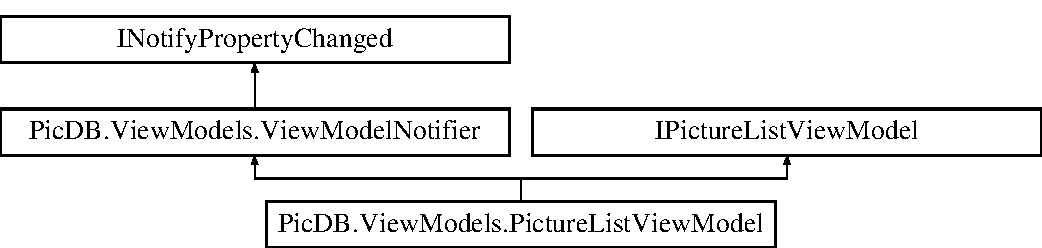
\includegraphics[height=3.000000cm]{class_pic_d_b_1_1_view_models_1_1_picture_list_view_model}
\end{center}
\end{figure}
\subsection*{Public Member Functions}
\begin{DoxyCompactItemize}
\item 
void \mbox{\hyperlink{class_pic_d_b_1_1_view_models_1_1_picture_list_view_model_a5225ed542833b5ce034f5ed1a19389af}{Reset\+List}} ()
\begin{DoxyCompactList}\small\item\em Resets a modified list to its original state. \end{DoxyCompactList}\item 
void \mbox{\hyperlink{class_pic_d_b_1_1_view_models_1_1_picture_list_view_model_a3fa38f6079f8dcf3122962ae515aa7d5}{Sync\+And\+Update\+Picture\+List}} ()
\begin{DoxyCompactList}\small\item\em Syncs the list with the database \end{DoxyCompactList}\end{DoxyCompactItemize}
\subsection*{Public Attributes}
\begin{DoxyCompactItemize}
\item 
I\+Enumerable$<$ I\+Picture\+View\+Model $>$ \mbox{\hyperlink{class_pic_d_b_1_1_view_models_1_1_picture_list_view_model_a7654958cbb50de3340aab1ffe55b06c6}{Prev\+Pictures}} =$>$ throw new Not\+Implemented\+Exception()
\begin{DoxyCompactList}\small\item\em O\+B\+S\+O\+L\+E\+TE\+: All prev. pictures to the current selected picture. \end{DoxyCompactList}\item 
I\+Enumerable$<$ I\+Picture\+View\+Model $>$ \mbox{\hyperlink{class_pic_d_b_1_1_view_models_1_1_picture_list_view_model_ac36598fb76dbcd1e2575fb97ff88a8c8}{Next\+Pictures}} =$>$ throw new Not\+Implemented\+Exception()
\begin{DoxyCompactList}\small\item\em O\+B\+S\+O\+L\+E\+TE\+: All next pictures to the current selected picture. \end{DoxyCompactList}\item 
int \mbox{\hyperlink{class_pic_d_b_1_1_view_models_1_1_picture_list_view_model_a935c7dd0503680824191cf2bf70c24e5}{Count}} =$>$ throw new Not\+Implemented\+Exception()
\begin{DoxyCompactList}\small\item\em O\+B\+S\+O\+L\+E\+TE\+: Number of all images \end{DoxyCompactList}\item 
int \mbox{\hyperlink{class_pic_d_b_1_1_view_models_1_1_picture_list_view_model_acbfd6df123842b3434df4e734aa1a4c8}{Current\+Index}} =$>$ throw new Not\+Implemented\+Exception()
\begin{DoxyCompactList}\small\item\em O\+B\+S\+O\+L\+E\+TE\+: The current Index, 1 based \end{DoxyCompactList}\item 
string \mbox{\hyperlink{class_pic_d_b_1_1_view_models_1_1_picture_list_view_model_ae7a8aacd98a0fdd5839c5c4b39e2263e}{Current\+Picture\+As\+String}} =$>$ throw new Not\+Implemented\+Exception()
\begin{DoxyCompactList}\small\item\em O\+B\+S\+O\+L\+E\+TE\+: \{Current\+Index\} of \{Cout\} \end{DoxyCompactList}\end{DoxyCompactItemize}
\subsection*{Properties}
\begin{DoxyCompactItemize}
\item 
I\+Picture\+View\+Model \mbox{\hyperlink{class_pic_d_b_1_1_view_models_1_1_picture_list_view_model_a0be4d92bdc6df25c70d3381d9858b184}{Current\+Picture}}\hspace{0.3cm}{\ttfamily  \mbox{[}get, set\mbox{]}}
\begin{DoxyCompactList}\small\item\em View\+Model of the current picture \end{DoxyCompactList}\item 
I\+Enumerable$<$ I\+Picture\+View\+Model $>$ \mbox{\hyperlink{class_pic_d_b_1_1_view_models_1_1_picture_list_view_model_a8889f6d5333a8d44a273776d92bba1b0}{List}}\hspace{0.3cm}{\ttfamily  \mbox{[}get, set\mbox{]}}
\begin{DoxyCompactList}\small\item\em List of all Picture\+View\+Models \end{DoxyCompactList}\end{DoxyCompactItemize}
\subsection*{Additional Inherited Members}


\subsection{Detailed Description}
View\+Model of a picture 



\subsection{Member Function Documentation}
\mbox{\Hypertarget{class_pic_d_b_1_1_view_models_1_1_picture_list_view_model_a5225ed542833b5ce034f5ed1a19389af}\label{class_pic_d_b_1_1_view_models_1_1_picture_list_view_model_a5225ed542833b5ce034f5ed1a19389af}} 
\index{Pic\+D\+B\+::\+View\+Models\+::\+Picture\+List\+View\+Model@{Pic\+D\+B\+::\+View\+Models\+::\+Picture\+List\+View\+Model}!Reset\+List@{Reset\+List}}
\index{Reset\+List@{Reset\+List}!Pic\+D\+B\+::\+View\+Models\+::\+Picture\+List\+View\+Model@{Pic\+D\+B\+::\+View\+Models\+::\+Picture\+List\+View\+Model}}
\subsubsection{\texorpdfstring{Reset\+List()}{ResetList()}}
{\footnotesize\ttfamily void Pic\+D\+B.\+View\+Models.\+Picture\+List\+View\+Model.\+Reset\+List (\begin{DoxyParamCaption}{ }\end{DoxyParamCaption})}



Resets a modified list to its original state. 

\mbox{\Hypertarget{class_pic_d_b_1_1_view_models_1_1_picture_list_view_model_a3fa38f6079f8dcf3122962ae515aa7d5}\label{class_pic_d_b_1_1_view_models_1_1_picture_list_view_model_a3fa38f6079f8dcf3122962ae515aa7d5}} 
\index{Pic\+D\+B\+::\+View\+Models\+::\+Picture\+List\+View\+Model@{Pic\+D\+B\+::\+View\+Models\+::\+Picture\+List\+View\+Model}!Sync\+And\+Update\+Picture\+List@{Sync\+And\+Update\+Picture\+List}}
\index{Sync\+And\+Update\+Picture\+List@{Sync\+And\+Update\+Picture\+List}!Pic\+D\+B\+::\+View\+Models\+::\+Picture\+List\+View\+Model@{Pic\+D\+B\+::\+View\+Models\+::\+Picture\+List\+View\+Model}}
\subsubsection{\texorpdfstring{Sync\+And\+Update\+Picture\+List()}{SyncAndUpdatePictureList()}}
{\footnotesize\ttfamily void Pic\+D\+B.\+View\+Models.\+Picture\+List\+View\+Model.\+Sync\+And\+Update\+Picture\+List (\begin{DoxyParamCaption}{ }\end{DoxyParamCaption})}



Syncs the list with the database 



\subsection{Member Data Documentation}
\mbox{\Hypertarget{class_pic_d_b_1_1_view_models_1_1_picture_list_view_model_a935c7dd0503680824191cf2bf70c24e5}\label{class_pic_d_b_1_1_view_models_1_1_picture_list_view_model_a935c7dd0503680824191cf2bf70c24e5}} 
\index{Pic\+D\+B\+::\+View\+Models\+::\+Picture\+List\+View\+Model@{Pic\+D\+B\+::\+View\+Models\+::\+Picture\+List\+View\+Model}!Count@{Count}}
\index{Count@{Count}!Pic\+D\+B\+::\+View\+Models\+::\+Picture\+List\+View\+Model@{Pic\+D\+B\+::\+View\+Models\+::\+Picture\+List\+View\+Model}}
\subsubsection{\texorpdfstring{Count}{Count}}
{\footnotesize\ttfamily int Pic\+D\+B.\+View\+Models.\+Picture\+List\+View\+Model.\+Count =$>$ throw new Not\+Implemented\+Exception()}



O\+B\+S\+O\+L\+E\+TE\+: Number of all images 

\mbox{\Hypertarget{class_pic_d_b_1_1_view_models_1_1_picture_list_view_model_acbfd6df123842b3434df4e734aa1a4c8}\label{class_pic_d_b_1_1_view_models_1_1_picture_list_view_model_acbfd6df123842b3434df4e734aa1a4c8}} 
\index{Pic\+D\+B\+::\+View\+Models\+::\+Picture\+List\+View\+Model@{Pic\+D\+B\+::\+View\+Models\+::\+Picture\+List\+View\+Model}!Current\+Index@{Current\+Index}}
\index{Current\+Index@{Current\+Index}!Pic\+D\+B\+::\+View\+Models\+::\+Picture\+List\+View\+Model@{Pic\+D\+B\+::\+View\+Models\+::\+Picture\+List\+View\+Model}}
\subsubsection{\texorpdfstring{Current\+Index}{CurrentIndex}}
{\footnotesize\ttfamily int Pic\+D\+B.\+View\+Models.\+Picture\+List\+View\+Model.\+Current\+Index =$>$ throw new Not\+Implemented\+Exception()}



O\+B\+S\+O\+L\+E\+TE\+: The current Index, 1 based 

\mbox{\Hypertarget{class_pic_d_b_1_1_view_models_1_1_picture_list_view_model_ae7a8aacd98a0fdd5839c5c4b39e2263e}\label{class_pic_d_b_1_1_view_models_1_1_picture_list_view_model_ae7a8aacd98a0fdd5839c5c4b39e2263e}} 
\index{Pic\+D\+B\+::\+View\+Models\+::\+Picture\+List\+View\+Model@{Pic\+D\+B\+::\+View\+Models\+::\+Picture\+List\+View\+Model}!Current\+Picture\+As\+String@{Current\+Picture\+As\+String}}
\index{Current\+Picture\+As\+String@{Current\+Picture\+As\+String}!Pic\+D\+B\+::\+View\+Models\+::\+Picture\+List\+View\+Model@{Pic\+D\+B\+::\+View\+Models\+::\+Picture\+List\+View\+Model}}
\subsubsection{\texorpdfstring{Current\+Picture\+As\+String}{CurrentPictureAsString}}
{\footnotesize\ttfamily string Pic\+D\+B.\+View\+Models.\+Picture\+List\+View\+Model.\+Current\+Picture\+As\+String =$>$ throw new Not\+Implemented\+Exception()}



O\+B\+S\+O\+L\+E\+TE\+: \{Current\+Index\} of \{Cout\} 

\mbox{\Hypertarget{class_pic_d_b_1_1_view_models_1_1_picture_list_view_model_ac36598fb76dbcd1e2575fb97ff88a8c8}\label{class_pic_d_b_1_1_view_models_1_1_picture_list_view_model_ac36598fb76dbcd1e2575fb97ff88a8c8}} 
\index{Pic\+D\+B\+::\+View\+Models\+::\+Picture\+List\+View\+Model@{Pic\+D\+B\+::\+View\+Models\+::\+Picture\+List\+View\+Model}!Next\+Pictures@{Next\+Pictures}}
\index{Next\+Pictures@{Next\+Pictures}!Pic\+D\+B\+::\+View\+Models\+::\+Picture\+List\+View\+Model@{Pic\+D\+B\+::\+View\+Models\+::\+Picture\+List\+View\+Model}}
\subsubsection{\texorpdfstring{Next\+Pictures}{NextPictures}}
{\footnotesize\ttfamily I\+Enumerable$<$I\+Picture\+View\+Model$>$ Pic\+D\+B.\+View\+Models.\+Picture\+List\+View\+Model.\+Next\+Pictures =$>$ throw new Not\+Implemented\+Exception()}



O\+B\+S\+O\+L\+E\+TE\+: All next pictures to the current selected picture. 

\mbox{\Hypertarget{class_pic_d_b_1_1_view_models_1_1_picture_list_view_model_a7654958cbb50de3340aab1ffe55b06c6}\label{class_pic_d_b_1_1_view_models_1_1_picture_list_view_model_a7654958cbb50de3340aab1ffe55b06c6}} 
\index{Pic\+D\+B\+::\+View\+Models\+::\+Picture\+List\+View\+Model@{Pic\+D\+B\+::\+View\+Models\+::\+Picture\+List\+View\+Model}!Prev\+Pictures@{Prev\+Pictures}}
\index{Prev\+Pictures@{Prev\+Pictures}!Pic\+D\+B\+::\+View\+Models\+::\+Picture\+List\+View\+Model@{Pic\+D\+B\+::\+View\+Models\+::\+Picture\+List\+View\+Model}}
\subsubsection{\texorpdfstring{Prev\+Pictures}{PrevPictures}}
{\footnotesize\ttfamily I\+Enumerable$<$I\+Picture\+View\+Model$>$ Pic\+D\+B.\+View\+Models.\+Picture\+List\+View\+Model.\+Prev\+Pictures =$>$ throw new Not\+Implemented\+Exception()}



O\+B\+S\+O\+L\+E\+TE\+: All prev. pictures to the current selected picture. 



\subsection{Property Documentation}
\mbox{\Hypertarget{class_pic_d_b_1_1_view_models_1_1_picture_list_view_model_a0be4d92bdc6df25c70d3381d9858b184}\label{class_pic_d_b_1_1_view_models_1_1_picture_list_view_model_a0be4d92bdc6df25c70d3381d9858b184}} 
\index{Pic\+D\+B\+::\+View\+Models\+::\+Picture\+List\+View\+Model@{Pic\+D\+B\+::\+View\+Models\+::\+Picture\+List\+View\+Model}!Current\+Picture@{Current\+Picture}}
\index{Current\+Picture@{Current\+Picture}!Pic\+D\+B\+::\+View\+Models\+::\+Picture\+List\+View\+Model@{Pic\+D\+B\+::\+View\+Models\+::\+Picture\+List\+View\+Model}}
\subsubsection{\texorpdfstring{Current\+Picture}{CurrentPicture}}
{\footnotesize\ttfamily I\+Picture\+View\+Model Pic\+D\+B.\+View\+Models.\+Picture\+List\+View\+Model.\+Current\+Picture\hspace{0.3cm}{\ttfamily [get]}, {\ttfamily [set]}}



View\+Model of the current picture 

\mbox{\Hypertarget{class_pic_d_b_1_1_view_models_1_1_picture_list_view_model_a8889f6d5333a8d44a273776d92bba1b0}\label{class_pic_d_b_1_1_view_models_1_1_picture_list_view_model_a8889f6d5333a8d44a273776d92bba1b0}} 
\index{Pic\+D\+B\+::\+View\+Models\+::\+Picture\+List\+View\+Model@{Pic\+D\+B\+::\+View\+Models\+::\+Picture\+List\+View\+Model}!List@{List}}
\index{List@{List}!Pic\+D\+B\+::\+View\+Models\+::\+Picture\+List\+View\+Model@{Pic\+D\+B\+::\+View\+Models\+::\+Picture\+List\+View\+Model}}
\subsubsection{\texorpdfstring{List}{List}}
{\footnotesize\ttfamily I\+Enumerable$<$I\+Picture\+View\+Model$>$ Pic\+D\+B.\+View\+Models.\+Picture\+List\+View\+Model.\+List\hspace{0.3cm}{\ttfamily [get]}, {\ttfamily [set]}}



List of all Picture\+View\+Models 



The documentation for this class was generated from the following file\+:\begin{DoxyCompactItemize}
\item 
C\+:/\+A\+A\+A-\/\+Technikum\+\_\+\+B\+W\+I/fourth\+Semester/\+S\+W\+E2/\+S\+W\+E2-\/\+C\+S/\+Pic\+D\+B/\+View\+Models/Picture\+List\+View\+Model.\+cs\end{DoxyCompactItemize}

\hypertarget{class_pic_d_b_1_1_models_1_1_picture_model}{}\section{Pic\+D\+B.\+Models.\+Picture\+Model Class Reference}
\label{class_pic_d_b_1_1_models_1_1_picture_model}\index{Pic\+D\+B.\+Models.\+Picture\+Model@{Pic\+D\+B.\+Models.\+Picture\+Model}}


Model of a picture  


Inheritance diagram for Pic\+D\+B.\+Models.\+Picture\+Model\+:\begin{figure}[H]
\begin{center}
\leavevmode
\includegraphics[height=2.000000cm]{class_pic_d_b_1_1_models_1_1_picture_model}
\end{center}
\end{figure}
\subsection*{Public Member Functions}
\begin{DoxyCompactItemize}
\item 
\mbox{\Hypertarget{class_pic_d_b_1_1_models_1_1_picture_model_a8f01ad2337a54ebc415871ae1941f596}\label{class_pic_d_b_1_1_models_1_1_picture_model_a8f01ad2337a54ebc415871ae1941f596}} 
{\bfseries Picture\+Model} (int \mbox{\hyperlink{class_pic_d_b_1_1_models_1_1_picture_model_a534920b39400aed29cff8e46d16f0643}{ID}})
\item 
\mbox{\Hypertarget{class_pic_d_b_1_1_models_1_1_picture_model_a3145355a21104b18f9db82d3ca7dd80d}\label{class_pic_d_b_1_1_models_1_1_picture_model_a3145355a21104b18f9db82d3ca7dd80d}} 
{\bfseries Picture\+Model} (string \mbox{\hyperlink{class_pic_d_b_1_1_models_1_1_picture_model_a1d64b84ae4e891844d1c2314f4addb62}{File\+Name}})
\item 
\mbox{\Hypertarget{class_pic_d_b_1_1_models_1_1_picture_model_a76f679543ac71baf433c9eba41166604}\label{class_pic_d_b_1_1_models_1_1_picture_model_a76f679543ac71baf433c9eba41166604}} 
{\bfseries Picture\+Model} (I\+Picture\+View\+Model view\+Model)
\end{DoxyCompactItemize}
\subsection*{Properties}
\begin{DoxyCompactItemize}
\item 
int \mbox{\hyperlink{class_pic_d_b_1_1_models_1_1_picture_model_a534920b39400aed29cff8e46d16f0643}{ID}}\hspace{0.3cm}{\ttfamily  \mbox{[}get, set\mbox{]}}
\begin{DoxyCompactList}\small\item\em Database primary key \end{DoxyCompactList}\item 
string \mbox{\hyperlink{class_pic_d_b_1_1_models_1_1_picture_model_a1d64b84ae4e891844d1c2314f4addb62}{File\+Name}}\hspace{0.3cm}{\ttfamily  \mbox{[}get, set\mbox{]}}
\begin{DoxyCompactList}\small\item\em File name, without path \end{DoxyCompactList}\item 
I\+I\+P\+T\+C\+Model \mbox{\hyperlink{class_pic_d_b_1_1_models_1_1_picture_model_a319a31a1a28094a01dcd9ab545379515}{I\+P\+TC}}\hspace{0.3cm}{\ttfamily  \mbox{[}get, set\mbox{]}}
\begin{DoxyCompactList}\small\item\em I\+P\+TC information \end{DoxyCompactList}\item 
I\+E\+X\+I\+F\+Model \mbox{\hyperlink{class_pic_d_b_1_1_models_1_1_picture_model_ae00785dc8fb8389d83a6c46b9da12e32}{E\+X\+IF}}\hspace{0.3cm}{\ttfamily  \mbox{[}get, set\mbox{]}}
\begin{DoxyCompactList}\small\item\em E\+X\+IF information \end{DoxyCompactList}\item 
I\+Camera\+Model \mbox{\hyperlink{class_pic_d_b_1_1_models_1_1_picture_model_a4b60e66ebee631a702fa5a9c833939af}{Camera}}\hspace{0.3cm}{\ttfamily  \mbox{[}get, set\mbox{]}}
\begin{DoxyCompactList}\small\item\em Camera \end{DoxyCompactList}\item 
I\+Photographer\+Model \mbox{\hyperlink{class_pic_d_b_1_1_models_1_1_picture_model_a57d74f8c86b80c2c9ddf34d86138b897}{Photographer}}\hspace{0.3cm}{\ttfamily  \mbox{[}get, set\mbox{]}}
\begin{DoxyCompactList}\small\item\em Photographer \end{DoxyCompactList}\end{DoxyCompactItemize}


\subsection{Detailed Description}
Model of a picture 



\subsection{Property Documentation}
\mbox{\Hypertarget{class_pic_d_b_1_1_models_1_1_picture_model_a4b60e66ebee631a702fa5a9c833939af}\label{class_pic_d_b_1_1_models_1_1_picture_model_a4b60e66ebee631a702fa5a9c833939af}} 
\index{Pic\+D\+B\+::\+Models\+::\+Picture\+Model@{Pic\+D\+B\+::\+Models\+::\+Picture\+Model}!Camera@{Camera}}
\index{Camera@{Camera}!Pic\+D\+B\+::\+Models\+::\+Picture\+Model@{Pic\+D\+B\+::\+Models\+::\+Picture\+Model}}
\subsubsection{\texorpdfstring{Camera}{Camera}}
{\footnotesize\ttfamily I\+Camera\+Model Pic\+D\+B.\+Models.\+Picture\+Model.\+Camera\hspace{0.3cm}{\ttfamily [get]}, {\ttfamily [set]}}



Camera 

\mbox{\Hypertarget{class_pic_d_b_1_1_models_1_1_picture_model_ae00785dc8fb8389d83a6c46b9da12e32}\label{class_pic_d_b_1_1_models_1_1_picture_model_ae00785dc8fb8389d83a6c46b9da12e32}} 
\index{Pic\+D\+B\+::\+Models\+::\+Picture\+Model@{Pic\+D\+B\+::\+Models\+::\+Picture\+Model}!E\+X\+IF@{E\+X\+IF}}
\index{E\+X\+IF@{E\+X\+IF}!Pic\+D\+B\+::\+Models\+::\+Picture\+Model@{Pic\+D\+B\+::\+Models\+::\+Picture\+Model}}
\subsubsection{\texorpdfstring{E\+X\+IF}{EXIF}}
{\footnotesize\ttfamily I\+E\+X\+I\+F\+Model Pic\+D\+B.\+Models.\+Picture\+Model.\+E\+X\+IF\hspace{0.3cm}{\ttfamily [get]}, {\ttfamily [set]}}



E\+X\+IF information 

\mbox{\Hypertarget{class_pic_d_b_1_1_models_1_1_picture_model_a1d64b84ae4e891844d1c2314f4addb62}\label{class_pic_d_b_1_1_models_1_1_picture_model_a1d64b84ae4e891844d1c2314f4addb62}} 
\index{Pic\+D\+B\+::\+Models\+::\+Picture\+Model@{Pic\+D\+B\+::\+Models\+::\+Picture\+Model}!File\+Name@{File\+Name}}
\index{File\+Name@{File\+Name}!Pic\+D\+B\+::\+Models\+::\+Picture\+Model@{Pic\+D\+B\+::\+Models\+::\+Picture\+Model}}
\subsubsection{\texorpdfstring{File\+Name}{FileName}}
{\footnotesize\ttfamily string Pic\+D\+B.\+Models.\+Picture\+Model.\+File\+Name\hspace{0.3cm}{\ttfamily [get]}, {\ttfamily [set]}}



File name, without path 

\mbox{\Hypertarget{class_pic_d_b_1_1_models_1_1_picture_model_a534920b39400aed29cff8e46d16f0643}\label{class_pic_d_b_1_1_models_1_1_picture_model_a534920b39400aed29cff8e46d16f0643}} 
\index{Pic\+D\+B\+::\+Models\+::\+Picture\+Model@{Pic\+D\+B\+::\+Models\+::\+Picture\+Model}!ID@{ID}}
\index{ID@{ID}!Pic\+D\+B\+::\+Models\+::\+Picture\+Model@{Pic\+D\+B\+::\+Models\+::\+Picture\+Model}}
\subsubsection{\texorpdfstring{ID}{ID}}
{\footnotesize\ttfamily int Pic\+D\+B.\+Models.\+Picture\+Model.\+ID\hspace{0.3cm}{\ttfamily [get]}, {\ttfamily [set]}}



Database primary key 

\mbox{\Hypertarget{class_pic_d_b_1_1_models_1_1_picture_model_a319a31a1a28094a01dcd9ab545379515}\label{class_pic_d_b_1_1_models_1_1_picture_model_a319a31a1a28094a01dcd9ab545379515}} 
\index{Pic\+D\+B\+::\+Models\+::\+Picture\+Model@{Pic\+D\+B\+::\+Models\+::\+Picture\+Model}!I\+P\+TC@{I\+P\+TC}}
\index{I\+P\+TC@{I\+P\+TC}!Pic\+D\+B\+::\+Models\+::\+Picture\+Model@{Pic\+D\+B\+::\+Models\+::\+Picture\+Model}}
\subsubsection{\texorpdfstring{I\+P\+TC}{IPTC}}
{\footnotesize\ttfamily I\+I\+P\+T\+C\+Model Pic\+D\+B.\+Models.\+Picture\+Model.\+I\+P\+TC\hspace{0.3cm}{\ttfamily [get]}, {\ttfamily [set]}}



I\+P\+TC information 

\mbox{\Hypertarget{class_pic_d_b_1_1_models_1_1_picture_model_a57d74f8c86b80c2c9ddf34d86138b897}\label{class_pic_d_b_1_1_models_1_1_picture_model_a57d74f8c86b80c2c9ddf34d86138b897}} 
\index{Pic\+D\+B\+::\+Models\+::\+Picture\+Model@{Pic\+D\+B\+::\+Models\+::\+Picture\+Model}!Photographer@{Photographer}}
\index{Photographer@{Photographer}!Pic\+D\+B\+::\+Models\+::\+Picture\+Model@{Pic\+D\+B\+::\+Models\+::\+Picture\+Model}}
\subsubsection{\texorpdfstring{Photographer}{Photographer}}
{\footnotesize\ttfamily I\+Photographer\+Model Pic\+D\+B.\+Models.\+Picture\+Model.\+Photographer\hspace{0.3cm}{\ttfamily [get]}, {\ttfamily [set]}}



Photographer 



The documentation for this class was generated from the following file\+:\begin{DoxyCompactItemize}
\item 
C\+:/\+A\+A\+A-\/\+Technikum\+\_\+\+B\+W\+I/fourth\+Semester/\+S\+W\+E2/\+S\+W\+E2-\/\+C\+S/\+Pic\+D\+B/\+Models/Picture\+Model.\+cs\end{DoxyCompactItemize}

\hypertarget{class_pic_d_b_1_1utils_1_1_exceptions_1_1_picture_not_found_exception}{}\section{Pic\+D\+B.\+utils.\+Exceptions.\+Picture\+Not\+Found\+Exception Class Reference}
\label{class_pic_d_b_1_1utils_1_1_exceptions_1_1_picture_not_found_exception}\index{Pic\+D\+B.\+utils.\+Exceptions.\+Picture\+Not\+Found\+Exception@{Pic\+D\+B.\+utils.\+Exceptions.\+Picture\+Not\+Found\+Exception}}
Inheritance diagram for Pic\+D\+B.\+utils.\+Exceptions.\+Picture\+Not\+Found\+Exception\+:\begin{figure}[H]
\begin{center}
\leavevmode
\includegraphics[height=2.000000cm]{class_pic_d_b_1_1utils_1_1_exceptions_1_1_picture_not_found_exception}
\end{center}
\end{figure}
\subsection*{Public Member Functions}
\begin{DoxyCompactItemize}
\item 
\mbox{\Hypertarget{class_pic_d_b_1_1utils_1_1_exceptions_1_1_picture_not_found_exception_a47ea61a22aa4771f0d5352e6f294fc4e}\label{class_pic_d_b_1_1utils_1_1_exceptions_1_1_picture_not_found_exception_a47ea61a22aa4771f0d5352e6f294fc4e}} 
{\bfseries Picture\+Not\+Found\+Exception} (string message)
\item 
\mbox{\Hypertarget{class_pic_d_b_1_1utils_1_1_exceptions_1_1_picture_not_found_exception_a344dc575a29ba98c38fced7ddc9190d2}\label{class_pic_d_b_1_1utils_1_1_exceptions_1_1_picture_not_found_exception_a344dc575a29ba98c38fced7ddc9190d2}} 
{\bfseries Picture\+Not\+Found\+Exception} (string message, Exception inner)
\end{DoxyCompactItemize}


The documentation for this class was generated from the following file\+:\begin{DoxyCompactItemize}
\item 
C\+:/\+A\+A\+A-\/\+Technikum\+\_\+\+B\+W\+I/fourth\+Semester/\+S\+W\+E2/\+S\+W\+E2-\/\+C\+S/\+Pic\+D\+B/utils/\+Exceptions/Picture\+Not\+Found\+Exception.\+cs\end{DoxyCompactItemize}

\hypertarget{class_pic_d_b_1_1_view_models_1_1_picture_view_model}{}\section{Pic\+D\+B.\+View\+Models.\+Picture\+View\+Model Class Reference}
\label{class_pic_d_b_1_1_view_models_1_1_picture_view_model}\index{Pic\+D\+B.\+View\+Models.\+Picture\+View\+Model@{Pic\+D\+B.\+View\+Models.\+Picture\+View\+Model}}


View\+Model of a picture  


Inheritance diagram for Pic\+D\+B.\+View\+Models.\+Picture\+View\+Model\+:\begin{figure}[H]
\begin{center}
\leavevmode
\includegraphics[height=3.000000cm]{class_pic_d_b_1_1_view_models_1_1_picture_view_model}
\end{center}
\end{figure}
\subsection*{Public Member Functions}
\begin{DoxyCompactItemize}
\item 
\mbox{\Hypertarget{class_pic_d_b_1_1_view_models_1_1_picture_view_model_a7b7e420f9cf6ffdb0700be4e117d47dd}\label{class_pic_d_b_1_1_view_models_1_1_picture_view_model_a7b7e420f9cf6ffdb0700be4e117d47dd}} 
{\bfseries Picture\+View\+Model} (I\+Picture\+Model model)
\end{DoxyCompactItemize}
\subsection*{Properties}
\begin{DoxyCompactItemize}
\item 
int \mbox{\hyperlink{class_pic_d_b_1_1_view_models_1_1_picture_view_model_a97814891952ce16bf7a1528fcd2216cd}{ID}}\hspace{0.3cm}{\ttfamily  \mbox{[}get, set\mbox{]}}
\begin{DoxyCompactList}\small\item\em Database primary key \end{DoxyCompactList}\item 
string \mbox{\hyperlink{class_pic_d_b_1_1_view_models_1_1_picture_view_model_ab678cd98ea07f4e746fa45d10637fcdc}{File\+Name}}\hspace{0.3cm}{\ttfamily  \mbox{[}get, set\mbox{]}}
\begin{DoxyCompactList}\small\item\em Name of the file \end{DoxyCompactList}\item 
string \mbox{\hyperlink{class_pic_d_b_1_1_view_models_1_1_picture_view_model_a6ddfcaf244162f0d6027f57ef6f753ae}{File\+Path}}\hspace{0.3cm}{\ttfamily  \mbox{[}get, set\mbox{]}}
\begin{DoxyCompactList}\small\item\em Full file path, used to load the image \end{DoxyCompactList}\item 
string \mbox{\hyperlink{class_pic_d_b_1_1_view_models_1_1_picture_view_model_a5f013b83aa58f2d4d4cfd35a53e00eb4}{Display\+Name}}\hspace{0.3cm}{\ttfamily  \mbox{[}get, set\mbox{]}}
\begin{DoxyCompactList}\small\item\em The line below the Picture. Format\+: \{I\+P\+T\+C.\+Headline$\vert$\+File\+Name\} (by \{Photographer$\vert$\+I\+P\+TC.By\+Line\}). \end{DoxyCompactList}\item 
I\+I\+P\+T\+C\+View\+Model \mbox{\hyperlink{class_pic_d_b_1_1_view_models_1_1_picture_view_model_a20d5866d8c026d9224b361249b92d657}{I\+P\+TC}}\hspace{0.3cm}{\ttfamily  \mbox{[}get, set\mbox{]}}
\begin{DoxyCompactList}\small\item\em The I\+P\+TC View\+Model \end{DoxyCompactList}\item 
I\+E\+X\+I\+F\+View\+Model \mbox{\hyperlink{class_pic_d_b_1_1_view_models_1_1_picture_view_model_a1963773b15fb44ed9f1b285c7dbb2ed1}{E\+X\+IF}}\hspace{0.3cm}{\ttfamily  \mbox{[}get, set\mbox{]}}
\begin{DoxyCompactList}\small\item\em The E\+X\+IF View\+Model \end{DoxyCompactList}\item 
I\+Photographer\+View\+Model \mbox{\hyperlink{class_pic_d_b_1_1_view_models_1_1_picture_view_model_aea991b658ad8d03f499fab158ff97b3e}{Photographer}}\hspace{0.3cm}{\ttfamily  \mbox{[}get, set\mbox{]}}
\begin{DoxyCompactList}\small\item\em The Photographer View\+Model \end{DoxyCompactList}\item 
I\+Camera\+View\+Model \mbox{\hyperlink{class_pic_d_b_1_1_view_models_1_1_picture_view_model_ad915e09a63dfe43eb4d324e0df024473}{Camera}}\hspace{0.3cm}{\ttfamily  \mbox{[}get, set\mbox{]}}
\begin{DoxyCompactList}\small\item\em The Camera View\+Model \end{DoxyCompactList}\end{DoxyCompactItemize}
\subsection*{Additional Inherited Members}


\subsection{Detailed Description}
View\+Model of a picture 



\subsection{Property Documentation}
\mbox{\Hypertarget{class_pic_d_b_1_1_view_models_1_1_picture_view_model_ad915e09a63dfe43eb4d324e0df024473}\label{class_pic_d_b_1_1_view_models_1_1_picture_view_model_ad915e09a63dfe43eb4d324e0df024473}} 
\index{Pic\+D\+B\+::\+View\+Models\+::\+Picture\+View\+Model@{Pic\+D\+B\+::\+View\+Models\+::\+Picture\+View\+Model}!Camera@{Camera}}
\index{Camera@{Camera}!Pic\+D\+B\+::\+View\+Models\+::\+Picture\+View\+Model@{Pic\+D\+B\+::\+View\+Models\+::\+Picture\+View\+Model}}
\subsubsection{\texorpdfstring{Camera}{Camera}}
{\footnotesize\ttfamily I\+Camera\+View\+Model Pic\+D\+B.\+View\+Models.\+Picture\+View\+Model.\+Camera\hspace{0.3cm}{\ttfamily [get]}, {\ttfamily [set]}}



The Camera View\+Model 

\mbox{\Hypertarget{class_pic_d_b_1_1_view_models_1_1_picture_view_model_a5f013b83aa58f2d4d4cfd35a53e00eb4}\label{class_pic_d_b_1_1_view_models_1_1_picture_view_model_a5f013b83aa58f2d4d4cfd35a53e00eb4}} 
\index{Pic\+D\+B\+::\+View\+Models\+::\+Picture\+View\+Model@{Pic\+D\+B\+::\+View\+Models\+::\+Picture\+View\+Model}!Display\+Name@{Display\+Name}}
\index{Display\+Name@{Display\+Name}!Pic\+D\+B\+::\+View\+Models\+::\+Picture\+View\+Model@{Pic\+D\+B\+::\+View\+Models\+::\+Picture\+View\+Model}}
\subsubsection{\texorpdfstring{Display\+Name}{DisplayName}}
{\footnotesize\ttfamily string Pic\+D\+B.\+View\+Models.\+Picture\+View\+Model.\+Display\+Name\hspace{0.3cm}{\ttfamily [get]}, {\ttfamily [set]}}



The line below the Picture. Format\+: \{I\+P\+T\+C.\+Headline$\vert$\+File\+Name\} (by \{Photographer$\vert$\+I\+P\+TC.By\+Line\}). 

\mbox{\Hypertarget{class_pic_d_b_1_1_view_models_1_1_picture_view_model_a1963773b15fb44ed9f1b285c7dbb2ed1}\label{class_pic_d_b_1_1_view_models_1_1_picture_view_model_a1963773b15fb44ed9f1b285c7dbb2ed1}} 
\index{Pic\+D\+B\+::\+View\+Models\+::\+Picture\+View\+Model@{Pic\+D\+B\+::\+View\+Models\+::\+Picture\+View\+Model}!E\+X\+IF@{E\+X\+IF}}
\index{E\+X\+IF@{E\+X\+IF}!Pic\+D\+B\+::\+View\+Models\+::\+Picture\+View\+Model@{Pic\+D\+B\+::\+View\+Models\+::\+Picture\+View\+Model}}
\subsubsection{\texorpdfstring{E\+X\+IF}{EXIF}}
{\footnotesize\ttfamily I\+E\+X\+I\+F\+View\+Model Pic\+D\+B.\+View\+Models.\+Picture\+View\+Model.\+E\+X\+IF\hspace{0.3cm}{\ttfamily [get]}, {\ttfamily [set]}}



The E\+X\+IF View\+Model 

\mbox{\Hypertarget{class_pic_d_b_1_1_view_models_1_1_picture_view_model_ab678cd98ea07f4e746fa45d10637fcdc}\label{class_pic_d_b_1_1_view_models_1_1_picture_view_model_ab678cd98ea07f4e746fa45d10637fcdc}} 
\index{Pic\+D\+B\+::\+View\+Models\+::\+Picture\+View\+Model@{Pic\+D\+B\+::\+View\+Models\+::\+Picture\+View\+Model}!File\+Name@{File\+Name}}
\index{File\+Name@{File\+Name}!Pic\+D\+B\+::\+View\+Models\+::\+Picture\+View\+Model@{Pic\+D\+B\+::\+View\+Models\+::\+Picture\+View\+Model}}
\subsubsection{\texorpdfstring{File\+Name}{FileName}}
{\footnotesize\ttfamily string Pic\+D\+B.\+View\+Models.\+Picture\+View\+Model.\+File\+Name\hspace{0.3cm}{\ttfamily [get]}, {\ttfamily [set]}}



Name of the file 

\mbox{\Hypertarget{class_pic_d_b_1_1_view_models_1_1_picture_view_model_a6ddfcaf244162f0d6027f57ef6f753ae}\label{class_pic_d_b_1_1_view_models_1_1_picture_view_model_a6ddfcaf244162f0d6027f57ef6f753ae}} 
\index{Pic\+D\+B\+::\+View\+Models\+::\+Picture\+View\+Model@{Pic\+D\+B\+::\+View\+Models\+::\+Picture\+View\+Model}!File\+Path@{File\+Path}}
\index{File\+Path@{File\+Path}!Pic\+D\+B\+::\+View\+Models\+::\+Picture\+View\+Model@{Pic\+D\+B\+::\+View\+Models\+::\+Picture\+View\+Model}}
\subsubsection{\texorpdfstring{File\+Path}{FilePath}}
{\footnotesize\ttfamily string Pic\+D\+B.\+View\+Models.\+Picture\+View\+Model.\+File\+Path\hspace{0.3cm}{\ttfamily [get]}, {\ttfamily [set]}}



Full file path, used to load the image 

\mbox{\Hypertarget{class_pic_d_b_1_1_view_models_1_1_picture_view_model_a97814891952ce16bf7a1528fcd2216cd}\label{class_pic_d_b_1_1_view_models_1_1_picture_view_model_a97814891952ce16bf7a1528fcd2216cd}} 
\index{Pic\+D\+B\+::\+View\+Models\+::\+Picture\+View\+Model@{Pic\+D\+B\+::\+View\+Models\+::\+Picture\+View\+Model}!ID@{ID}}
\index{ID@{ID}!Pic\+D\+B\+::\+View\+Models\+::\+Picture\+View\+Model@{Pic\+D\+B\+::\+View\+Models\+::\+Picture\+View\+Model}}
\subsubsection{\texorpdfstring{ID}{ID}}
{\footnotesize\ttfamily int Pic\+D\+B.\+View\+Models.\+Picture\+View\+Model.\+ID\hspace{0.3cm}{\ttfamily [get]}, {\ttfamily [set]}}



Database primary key 

\mbox{\Hypertarget{class_pic_d_b_1_1_view_models_1_1_picture_view_model_a20d5866d8c026d9224b361249b92d657}\label{class_pic_d_b_1_1_view_models_1_1_picture_view_model_a20d5866d8c026d9224b361249b92d657}} 
\index{Pic\+D\+B\+::\+View\+Models\+::\+Picture\+View\+Model@{Pic\+D\+B\+::\+View\+Models\+::\+Picture\+View\+Model}!I\+P\+TC@{I\+P\+TC}}
\index{I\+P\+TC@{I\+P\+TC}!Pic\+D\+B\+::\+View\+Models\+::\+Picture\+View\+Model@{Pic\+D\+B\+::\+View\+Models\+::\+Picture\+View\+Model}}
\subsubsection{\texorpdfstring{I\+P\+TC}{IPTC}}
{\footnotesize\ttfamily I\+I\+P\+T\+C\+View\+Model Pic\+D\+B.\+View\+Models.\+Picture\+View\+Model.\+I\+P\+TC\hspace{0.3cm}{\ttfamily [get]}, {\ttfamily [set]}}



The I\+P\+TC View\+Model 

\mbox{\Hypertarget{class_pic_d_b_1_1_view_models_1_1_picture_view_model_aea991b658ad8d03f499fab158ff97b3e}\label{class_pic_d_b_1_1_view_models_1_1_picture_view_model_aea991b658ad8d03f499fab158ff97b3e}} 
\index{Pic\+D\+B\+::\+View\+Models\+::\+Picture\+View\+Model@{Pic\+D\+B\+::\+View\+Models\+::\+Picture\+View\+Model}!Photographer@{Photographer}}
\index{Photographer@{Photographer}!Pic\+D\+B\+::\+View\+Models\+::\+Picture\+View\+Model@{Pic\+D\+B\+::\+View\+Models\+::\+Picture\+View\+Model}}
\subsubsection{\texorpdfstring{Photographer}{Photographer}}
{\footnotesize\ttfamily I\+Photographer\+View\+Model Pic\+D\+B.\+View\+Models.\+Picture\+View\+Model.\+Photographer\hspace{0.3cm}{\ttfamily [get]}, {\ttfamily [set]}}



The Photographer View\+Model 



The documentation for this class was generated from the following file\+:\begin{DoxyCompactItemize}
\item 
C\+:/\+A\+A\+A-\/\+Technikum\+\_\+\+B\+W\+I/fourth\+Semester/\+S\+W\+E2/\+S\+W\+E2-\/\+C\+S/\+Pic\+D\+B/\+View\+Models/Picture\+View\+Model.\+cs\end{DoxyCompactItemize}

\hypertarget{class_pic_d_b_1_1_view_models_1_1_search_view_model}{}\section{Pic\+D\+B.\+View\+Models.\+Search\+View\+Model Class Reference}
\label{class_pic_d_b_1_1_view_models_1_1_search_view_model}\index{Pic\+D\+B.\+View\+Models.\+Search\+View\+Model@{Pic\+D\+B.\+View\+Models.\+Search\+View\+Model}}


View\+Model of searchbar  


Inheritance diagram for Pic\+D\+B.\+View\+Models.\+Search\+View\+Model\+:\begin{figure}[H]
\begin{center}
\leavevmode
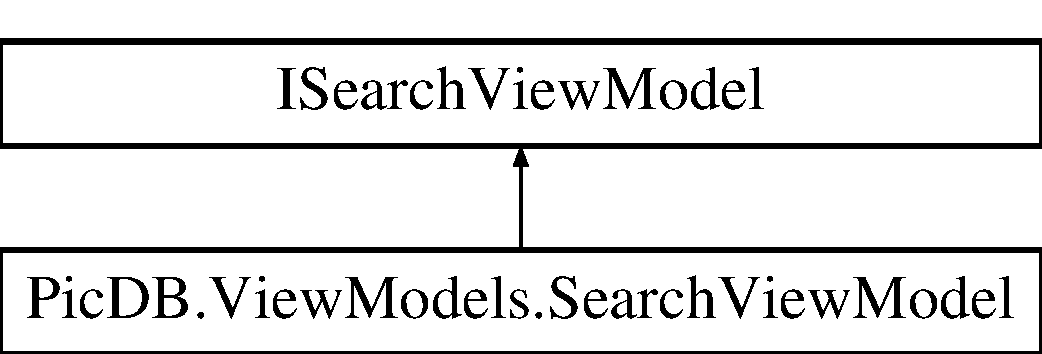
\includegraphics[height=2.000000cm]{class_pic_d_b_1_1_view_models_1_1_search_view_model}
\end{center}
\end{figure}
\subsection*{Properties}
\begin{DoxyCompactItemize}
\item 
string \mbox{\hyperlink{class_pic_d_b_1_1_view_models_1_1_search_view_model_aeba05756675efaf7ce63d22d19215231}{Search\+Text}}\hspace{0.3cm}{\ttfamily  \mbox{[}get, set\mbox{]}}
\begin{DoxyCompactList}\small\item\em The search text \end{DoxyCompactList}\item 
bool \mbox{\hyperlink{class_pic_d_b_1_1_view_models_1_1_search_view_model_ac182a20e1f3d07d041057228d1c265b0}{Is\+Active}}\hspace{0.3cm}{\ttfamily  \mbox{[}get\mbox{]}}
\begin{DoxyCompactList}\small\item\em True, if a search is active \end{DoxyCompactList}\item 
int \mbox{\hyperlink{class_pic_d_b_1_1_view_models_1_1_search_view_model_ab0b96a30c200f0e7ba85241bcfce82c7}{Result\+Count}}\hspace{0.3cm}{\ttfamily  \mbox{[}get, set\mbox{]}}
\begin{DoxyCompactList}\small\item\em Number of photos found. \end{DoxyCompactList}\end{DoxyCompactItemize}


\subsection{Detailed Description}
View\+Model of searchbar 



\subsection{Property Documentation}
\mbox{\Hypertarget{class_pic_d_b_1_1_view_models_1_1_search_view_model_ac182a20e1f3d07d041057228d1c265b0}\label{class_pic_d_b_1_1_view_models_1_1_search_view_model_ac182a20e1f3d07d041057228d1c265b0}} 
\index{Pic\+D\+B\+::\+View\+Models\+::\+Search\+View\+Model@{Pic\+D\+B\+::\+View\+Models\+::\+Search\+View\+Model}!Is\+Active@{Is\+Active}}
\index{Is\+Active@{Is\+Active}!Pic\+D\+B\+::\+View\+Models\+::\+Search\+View\+Model@{Pic\+D\+B\+::\+View\+Models\+::\+Search\+View\+Model}}
\subsubsection{\texorpdfstring{Is\+Active}{IsActive}}
{\footnotesize\ttfamily bool Pic\+D\+B.\+View\+Models.\+Search\+View\+Model.\+Is\+Active\hspace{0.3cm}{\ttfamily [get]}}



True, if a search is active 

\mbox{\Hypertarget{class_pic_d_b_1_1_view_models_1_1_search_view_model_ab0b96a30c200f0e7ba85241bcfce82c7}\label{class_pic_d_b_1_1_view_models_1_1_search_view_model_ab0b96a30c200f0e7ba85241bcfce82c7}} 
\index{Pic\+D\+B\+::\+View\+Models\+::\+Search\+View\+Model@{Pic\+D\+B\+::\+View\+Models\+::\+Search\+View\+Model}!Result\+Count@{Result\+Count}}
\index{Result\+Count@{Result\+Count}!Pic\+D\+B\+::\+View\+Models\+::\+Search\+View\+Model@{Pic\+D\+B\+::\+View\+Models\+::\+Search\+View\+Model}}
\subsubsection{\texorpdfstring{Result\+Count}{ResultCount}}
{\footnotesize\ttfamily int Pic\+D\+B.\+View\+Models.\+Search\+View\+Model.\+Result\+Count\hspace{0.3cm}{\ttfamily [get]}, {\ttfamily [set]}}



Number of photos found. 

\mbox{\Hypertarget{class_pic_d_b_1_1_view_models_1_1_search_view_model_aeba05756675efaf7ce63d22d19215231}\label{class_pic_d_b_1_1_view_models_1_1_search_view_model_aeba05756675efaf7ce63d22d19215231}} 
\index{Pic\+D\+B\+::\+View\+Models\+::\+Search\+View\+Model@{Pic\+D\+B\+::\+View\+Models\+::\+Search\+View\+Model}!Search\+Text@{Search\+Text}}
\index{Search\+Text@{Search\+Text}!Pic\+D\+B\+::\+View\+Models\+::\+Search\+View\+Model@{Pic\+D\+B\+::\+View\+Models\+::\+Search\+View\+Model}}
\subsubsection{\texorpdfstring{Search\+Text}{SearchText}}
{\footnotesize\ttfamily string Pic\+D\+B.\+View\+Models.\+Search\+View\+Model.\+Search\+Text\hspace{0.3cm}{\ttfamily [get]}, {\ttfamily [set]}}



The search text 



The documentation for this class was generated from the following file\+:\begin{DoxyCompactItemize}
\item 
C\+:/\+A\+A\+A-\/\+Technikum\+\_\+\+B\+W\+I/fourth\+Semester/\+S\+W\+E2/\+S\+W\+E2-\/\+C\+S/\+Pic\+D\+B/\+View\+Models/Search\+View\+Model.\+cs\end{DoxyCompactItemize}

\hypertarget{class_pic_d_b_1_1_uebungen_1_1_u_e_b1}{}\section{Pic\+D\+B.\+Uebungen.\+U\+E\+B1 Class Reference}
\label{class_pic_d_b_1_1_uebungen_1_1_u_e_b1}\index{Pic\+D\+B.\+Uebungen.\+U\+E\+B1@{Pic\+D\+B.\+Uebungen.\+U\+E\+B1}}
Inheritance diagram for Pic\+D\+B.\+Uebungen.\+U\+E\+B1\+:\begin{figure}[H]
\begin{center}
\leavevmode
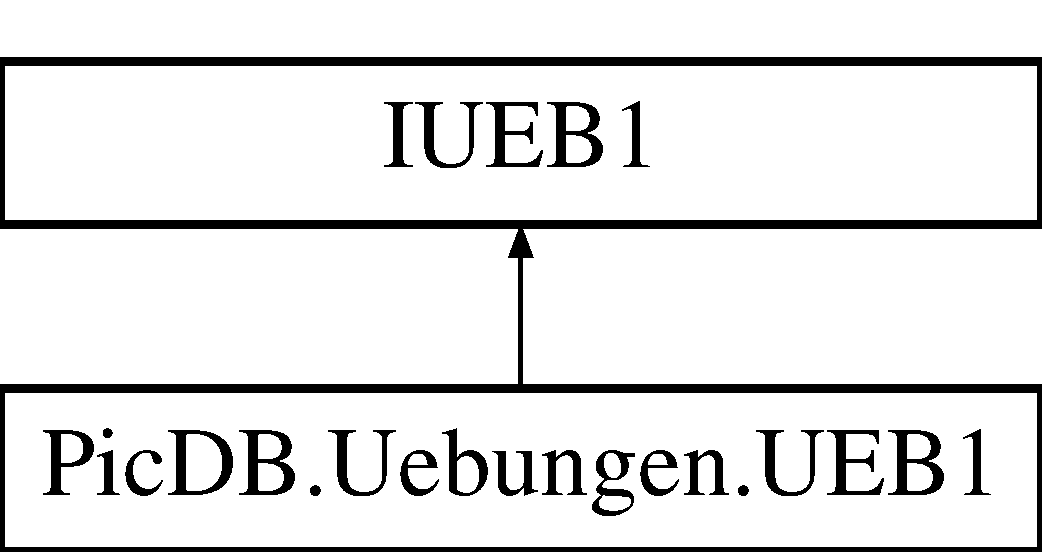
\includegraphics[height=2.000000cm]{class_pic_d_b_1_1_uebungen_1_1_u_e_b1}
\end{center}
\end{figure}
\subsection*{Public Member Functions}
\begin{DoxyCompactItemize}
\item 
\mbox{\Hypertarget{class_pic_d_b_1_1_uebungen_1_1_u_e_b1_a11d5688afbaf21a2c67b0821e6924e9a}\label{class_pic_d_b_1_1_uebungen_1_1_u_e_b1_a11d5688afbaf21a2c67b0821e6924e9a}} 
I\+Application {\bfseries Get\+Application} ()
\item 
\mbox{\Hypertarget{class_pic_d_b_1_1_uebungen_1_1_u_e_b1_a4bc80c1c20ac8006c52fcb578619d6b6}\label{class_pic_d_b_1_1_uebungen_1_1_u_e_b1_a4bc80c1c20ac8006c52fcb578619d6b6}} 
void {\bfseries Hello\+World} ()
\item 
\mbox{\Hypertarget{class_pic_d_b_1_1_uebungen_1_1_u_e_b1_ac5deae83945348cf375acf1742414cf9}\label{class_pic_d_b_1_1_uebungen_1_1_u_e_b1_ac5deae83945348cf375acf1742414cf9}} 
I\+Data\+Access\+Layer {\bfseries Get\+Any\+Data\+Access\+Layer} ()
\item 
\mbox{\Hypertarget{class_pic_d_b_1_1_uebungen_1_1_u_e_b1_ab99b09a8a65554655fc5023a071dcdb6}\label{class_pic_d_b_1_1_uebungen_1_1_u_e_b1_ab99b09a8a65554655fc5023a071dcdb6}} 
I\+Business\+Layer {\bfseries Get\+Business\+Layer} ()
\item 
\mbox{\Hypertarget{class_pic_d_b_1_1_uebungen_1_1_u_e_b1_afcd9e2bf3a60d543f451401b4f7b487f}\label{class_pic_d_b_1_1_uebungen_1_1_u_e_b1_afcd9e2bf3a60d543f451401b4f7b487f}} 
B\+I\+F.\+S\+W\+E2.\+Interfaces.\+Models.\+I\+E\+X\+I\+F\+Model {\bfseries Get\+Empty\+E\+X\+I\+F\+Model} ()
\item 
\mbox{\Hypertarget{class_pic_d_b_1_1_uebungen_1_1_u_e_b1_a92785e1d6d947bd38403fe5cca0f094e}\label{class_pic_d_b_1_1_uebungen_1_1_u_e_b1_a92785e1d6d947bd38403fe5cca0f094e}} 
B\+I\+F.\+S\+W\+E2.\+Interfaces.\+View\+Models.\+I\+E\+X\+I\+F\+View\+Model {\bfseries Get\+Empty\+E\+X\+I\+F\+View\+Model} ()
\item 
\mbox{\Hypertarget{class_pic_d_b_1_1_uebungen_1_1_u_e_b1_a9cf6988136cf089da287ea00fece7fd0}\label{class_pic_d_b_1_1_uebungen_1_1_u_e_b1_a9cf6988136cf089da287ea00fece7fd0}} 
B\+I\+F.\+S\+W\+E2.\+Interfaces.\+Models.\+I\+I\+P\+T\+C\+Model {\bfseries Get\+Empty\+I\+P\+T\+C\+Model} ()
\item 
\mbox{\Hypertarget{class_pic_d_b_1_1_uebungen_1_1_u_e_b1_a8c76d498934bc0497d7b23177d25b00a}\label{class_pic_d_b_1_1_uebungen_1_1_u_e_b1_a8c76d498934bc0497d7b23177d25b00a}} 
B\+I\+F.\+S\+W\+E2.\+Interfaces.\+View\+Models.\+I\+I\+P\+T\+C\+View\+Model {\bfseries Get\+Empty\+I\+P\+T\+C\+View\+Model} ()
\item 
\mbox{\Hypertarget{class_pic_d_b_1_1_uebungen_1_1_u_e_b1_aab0e273a2d0c7692467ecdc365541e9c}\label{class_pic_d_b_1_1_uebungen_1_1_u_e_b1_aab0e273a2d0c7692467ecdc365541e9c}} 
B\+I\+F.\+S\+W\+E2.\+Interfaces.\+View\+Models.\+I\+Main\+Window\+View\+Model {\bfseries Get\+Empty\+Main\+Window\+View\+Model} ()
\item 
\mbox{\Hypertarget{class_pic_d_b_1_1_uebungen_1_1_u_e_b1_ac47dbc876c9d4b6b4a73cc8970adc4e3}\label{class_pic_d_b_1_1_uebungen_1_1_u_e_b1_ac47dbc876c9d4b6b4a73cc8970adc4e3}} 
B\+I\+F.\+S\+W\+E2.\+Interfaces.\+View\+Models.\+I\+Photographer\+List\+View\+Model {\bfseries Get\+Empty\+Photographer\+List\+View\+Model} ()
\item 
\mbox{\Hypertarget{class_pic_d_b_1_1_uebungen_1_1_u_e_b1_ad20e9e764e42c478517d0770198fe705}\label{class_pic_d_b_1_1_uebungen_1_1_u_e_b1_ad20e9e764e42c478517d0770198fe705}} 
B\+I\+F.\+S\+W\+E2.\+Interfaces.\+Models.\+I\+Photographer\+Model {\bfseries Get\+Empty\+Photographer\+Model} ()
\item 
\mbox{\Hypertarget{class_pic_d_b_1_1_uebungen_1_1_u_e_b1_ac3ae5196472bee80f52a2fd25a36709d}\label{class_pic_d_b_1_1_uebungen_1_1_u_e_b1_ac3ae5196472bee80f52a2fd25a36709d}} 
B\+I\+F.\+S\+W\+E2.\+Interfaces.\+View\+Models.\+I\+Photographer\+View\+Model {\bfseries Get\+Empty\+Photographer\+View\+Model} ()
\item 
\mbox{\Hypertarget{class_pic_d_b_1_1_uebungen_1_1_u_e_b1_a00f53ea2e7a2d1d3625d5a176c757174}\label{class_pic_d_b_1_1_uebungen_1_1_u_e_b1_a00f53ea2e7a2d1d3625d5a176c757174}} 
B\+I\+F.\+S\+W\+E2.\+Interfaces.\+View\+Models.\+I\+Picture\+List\+View\+Model {\bfseries Get\+Empty\+Picture\+List\+View\+Model} ()
\item 
\mbox{\Hypertarget{class_pic_d_b_1_1_uebungen_1_1_u_e_b1_af02fdb670055bfe8377f5d9fef7d2b72}\label{class_pic_d_b_1_1_uebungen_1_1_u_e_b1_af02fdb670055bfe8377f5d9fef7d2b72}} 
B\+I\+F.\+S\+W\+E2.\+Interfaces.\+Models.\+I\+Picture\+Model {\bfseries Get\+Empty\+Picture\+Model} ()
\item 
\mbox{\Hypertarget{class_pic_d_b_1_1_uebungen_1_1_u_e_b1_a73bc371fefee7094c408c2c8b8ba9e01}\label{class_pic_d_b_1_1_uebungen_1_1_u_e_b1_a73bc371fefee7094c408c2c8b8ba9e01}} 
B\+I\+F.\+S\+W\+E2.\+Interfaces.\+View\+Models.\+I\+Picture\+View\+Model {\bfseries Get\+Empty\+Picture\+View\+Model} ()
\item 
\mbox{\Hypertarget{class_pic_d_b_1_1_uebungen_1_1_u_e_b1_a78830b2ea7ec7cf5be9b2f8bb75cefee}\label{class_pic_d_b_1_1_uebungen_1_1_u_e_b1_a78830b2ea7ec7cf5be9b2f8bb75cefee}} 
B\+I\+F.\+S\+W\+E2.\+Interfaces.\+View\+Models.\+I\+Search\+View\+Model {\bfseries Get\+Empty\+Search\+View\+Model} ()
\item 
\mbox{\Hypertarget{class_pic_d_b_1_1_uebungen_1_1_u_e_b1_a2e8cba6371dc4355126680d5ae99e300}\label{class_pic_d_b_1_1_uebungen_1_1_u_e_b1_a2e8cba6371dc4355126680d5ae99e300}} 
void {\bfseries Test\+Setup} (string picture\+Path)
\item 
\mbox{\Hypertarget{class_pic_d_b_1_1_uebungen_1_1_u_e_b1_a9e2beee761b73a45d17babb2c884a4b6}\label{class_pic_d_b_1_1_uebungen_1_1_u_e_b1_a9e2beee761b73a45d17babb2c884a4b6}} 
I\+Camera\+Model {\bfseries Get\+Empty\+Camera\+Model} ()
\item 
\mbox{\Hypertarget{class_pic_d_b_1_1_uebungen_1_1_u_e_b1_aea7762ec1b242e86db3b16637c4be8b1}\label{class_pic_d_b_1_1_uebungen_1_1_u_e_b1_aea7762ec1b242e86db3b16637c4be8b1}} 
I\+Camera\+List\+View\+Model {\bfseries Get\+Empty\+Camera\+List\+View\+Model} ()
\item 
\mbox{\Hypertarget{class_pic_d_b_1_1_uebungen_1_1_u_e_b1_a7882d9be85be13222065022a89e8a394}\label{class_pic_d_b_1_1_uebungen_1_1_u_e_b1_a7882d9be85be13222065022a89e8a394}} 
I\+Camera\+View\+Model {\bfseries Get\+Empty\+Camera\+View\+Model} ()
\end{DoxyCompactItemize}


The documentation for this class was generated from the following file\+:\begin{DoxyCompactItemize}
\item 
C\+:/\+A\+A\+A-\/\+Technikum\+\_\+\+B\+W\+I/fourth\+Semester/\+S\+W\+E2/\+S\+W\+E2-\/\+C\+S/\+Pic\+D\+B/\+Uebungen/U\+E\+B1.\+cs\end{DoxyCompactItemize}

\hypertarget{class_pic_d_b_1_1_uebungen_1_1_u_e_b2}{}\section{Pic\+D\+B.\+Uebungen.\+U\+E\+B2 Class Reference}
\label{class_pic_d_b_1_1_uebungen_1_1_u_e_b2}\index{Pic\+D\+B.\+Uebungen.\+U\+E\+B2@{Pic\+D\+B.\+Uebungen.\+U\+E\+B2}}
Inheritance diagram for Pic\+D\+B.\+Uebungen.\+U\+E\+B2\+:\begin{figure}[H]
\begin{center}
\leavevmode
\includegraphics[height=2.000000cm]{class_pic_d_b_1_1_uebungen_1_1_u_e_b2}
\end{center}
\end{figure}
\subsection*{Public Member Functions}
\begin{DoxyCompactItemize}
\item 
\mbox{\Hypertarget{class_pic_d_b_1_1_uebungen_1_1_u_e_b2_a8d5b9d8ccdf8e62fe2ec1ff860c3248d}\label{class_pic_d_b_1_1_uebungen_1_1_u_e_b2_a8d5b9d8ccdf8e62fe2ec1ff860c3248d}} 
void {\bfseries Hello\+World} ()
\item 
\mbox{\Hypertarget{class_pic_d_b_1_1_uebungen_1_1_u_e_b2_a93d810ef8a680dd1b112306cdd1eb3b7}\label{class_pic_d_b_1_1_uebungen_1_1_u_e_b2_a93d810ef8a680dd1b112306cdd1eb3b7}} 
I\+Business\+Layer {\bfseries Get\+Business\+Layer} ()
\item 
\mbox{\Hypertarget{class_pic_d_b_1_1_uebungen_1_1_u_e_b2_a5ba6e0701ae149ee5167049b5331079d}\label{class_pic_d_b_1_1_uebungen_1_1_u_e_b2_a5ba6e0701ae149ee5167049b5331079d}} 
B\+I\+F.\+S\+W\+E2.\+Interfaces.\+View\+Models.\+I\+Main\+Window\+View\+Model {\bfseries Get\+Main\+Window\+View\+Model} ()
\item 
\mbox{\Hypertarget{class_pic_d_b_1_1_uebungen_1_1_u_e_b2_af42a6b204020ed0b829bea5156740b1b}\label{class_pic_d_b_1_1_uebungen_1_1_u_e_b2_af42a6b204020ed0b829bea5156740b1b}} 
B\+I\+F.\+S\+W\+E2.\+Interfaces.\+Models.\+I\+Picture\+Model {\bfseries Get\+Picture\+Model} (string filename)
\item 
\mbox{\Hypertarget{class_pic_d_b_1_1_uebungen_1_1_u_e_b2_ad32bc53be5b805a360389a78da4e916b}\label{class_pic_d_b_1_1_uebungen_1_1_u_e_b2_ad32bc53be5b805a360389a78da4e916b}} 
B\+I\+F.\+S\+W\+E2.\+Interfaces.\+View\+Models.\+I\+Picture\+View\+Model {\bfseries Get\+Picture\+View\+Model} (B\+I\+F.\+S\+W\+E2.\+Interfaces.\+Models.\+I\+Picture\+Model mdl)
\item 
\mbox{\Hypertarget{class_pic_d_b_1_1_uebungen_1_1_u_e_b2_a515cc0cacdca52659740afd1d31ec97e}\label{class_pic_d_b_1_1_uebungen_1_1_u_e_b2_a515cc0cacdca52659740afd1d31ec97e}} 
void {\bfseries Test\+Setup} (string picture\+Path)
\item 
\mbox{\Hypertarget{class_pic_d_b_1_1_uebungen_1_1_u_e_b2_a6d7921a4addcded9c95ef87f32fbcf39}\label{class_pic_d_b_1_1_uebungen_1_1_u_e_b2_a6d7921a4addcded9c95ef87f32fbcf39}} 
I\+Camera\+Model {\bfseries Get\+Camera\+Model} (string producer, string make)
\item 
\mbox{\Hypertarget{class_pic_d_b_1_1_uebungen_1_1_u_e_b2_a138207dd8e5d31f32257dee101da58fa}\label{class_pic_d_b_1_1_uebungen_1_1_u_e_b2_a138207dd8e5d31f32257dee101da58fa}} 
I\+Camera\+View\+Model {\bfseries Get\+Camera\+View\+Model} (I\+Camera\+Model mdl)
\end{DoxyCompactItemize}


The documentation for this class was generated from the following file\+:\begin{DoxyCompactItemize}
\item 
C\+:/\+A\+A\+A-\/\+Technikum\+\_\+\+B\+W\+I/fourth\+Semester/\+S\+W\+E2/\+S\+W\+E2-\/\+C\+S/\+Pic\+D\+B/\+Uebungen/U\+E\+B2.\+cs\end{DoxyCompactItemize}

\hypertarget{class_pic_d_b_1_1_uebungen_1_1_u_e_b3}{}\section{Pic\+D\+B.\+Uebungen.\+U\+E\+B3 Class Reference}
\label{class_pic_d_b_1_1_uebungen_1_1_u_e_b3}\index{Pic\+D\+B.\+Uebungen.\+U\+E\+B3@{Pic\+D\+B.\+Uebungen.\+U\+E\+B3}}
Inheritance diagram for Pic\+D\+B.\+Uebungen.\+U\+E\+B3\+:\begin{figure}[H]
\begin{center}
\leavevmode
\includegraphics[height=2.000000cm]{class_pic_d_b_1_1_uebungen_1_1_u_e_b3}
\end{center}
\end{figure}
\subsection*{Public Member Functions}
\begin{DoxyCompactItemize}
\item 
\mbox{\Hypertarget{class_pic_d_b_1_1_uebungen_1_1_u_e_b3_acd8a743eeed9a63c337f008a395d1856}\label{class_pic_d_b_1_1_uebungen_1_1_u_e_b3_acd8a743eeed9a63c337f008a395d1856}} 
void {\bfseries Hello\+World} ()
\item 
\mbox{\Hypertarget{class_pic_d_b_1_1_uebungen_1_1_u_e_b3_a6da8a75a5d2b2914e9cb07f2e6c702b9}\label{class_pic_d_b_1_1_uebungen_1_1_u_e_b3_a6da8a75a5d2b2914e9cb07f2e6c702b9}} 
I\+Business\+Layer {\bfseries Get\+Business\+Layer} ()
\item 
\mbox{\Hypertarget{class_pic_d_b_1_1_uebungen_1_1_u_e_b3_a8a26b28b142543d2145e052e018ac098}\label{class_pic_d_b_1_1_uebungen_1_1_u_e_b3_a8a26b28b142543d2145e052e018ac098}} 
void {\bfseries Test\+Setup} (string picture\+Path)
\item 
\mbox{\Hypertarget{class_pic_d_b_1_1_uebungen_1_1_u_e_b3_a579cfdc62d8e9ebeb9c62102acaaf731}\label{class_pic_d_b_1_1_uebungen_1_1_u_e_b3_a579cfdc62d8e9ebeb9c62102acaaf731}} 
I\+Data\+Access\+Layer {\bfseries Get\+Data\+Access\+Layer} ()
\item 
\mbox{\Hypertarget{class_pic_d_b_1_1_uebungen_1_1_u_e_b3_a3d58b17cf0c092c9f77508c46dfef731}\label{class_pic_d_b_1_1_uebungen_1_1_u_e_b3_a3d58b17cf0c092c9f77508c46dfef731}} 
I\+Search\+View\+Model {\bfseries Get\+Search\+View\+Model} ()
\end{DoxyCompactItemize}


The documentation for this class was generated from the following file\+:\begin{DoxyCompactItemize}
\item 
C\+:/\+A\+A\+A-\/\+Technikum\+\_\+\+B\+W\+I/fourth\+Semester/\+S\+W\+E2/\+S\+W\+E2-\/\+C\+S/\+Pic\+D\+B/\+Uebungen/U\+E\+B3.\+cs\end{DoxyCompactItemize}

\hypertarget{class_pic_d_b_1_1_uebungen_1_1_u_e_b4}{}\section{Pic\+D\+B.\+Uebungen.\+U\+E\+B4 Class Reference}
\label{class_pic_d_b_1_1_uebungen_1_1_u_e_b4}\index{Pic\+D\+B.\+Uebungen.\+U\+E\+B4@{Pic\+D\+B.\+Uebungen.\+U\+E\+B4}}
Inheritance diagram for Pic\+D\+B.\+Uebungen.\+U\+E\+B4\+:\begin{figure}[H]
\begin{center}
\leavevmode
\includegraphics[height=2.000000cm]{class_pic_d_b_1_1_uebungen_1_1_u_e_b4}
\end{center}
\end{figure}
\subsection*{Public Member Functions}
\begin{DoxyCompactItemize}
\item 
\mbox{\Hypertarget{class_pic_d_b_1_1_uebungen_1_1_u_e_b4_ad29c2052f9868e0efa2a46eb2262c263}\label{class_pic_d_b_1_1_uebungen_1_1_u_e_b4_ad29c2052f9868e0efa2a46eb2262c263}} 
void {\bfseries Hello\+World} ()
\item 
\mbox{\Hypertarget{class_pic_d_b_1_1_uebungen_1_1_u_e_b4_a7db95feb7619301f3676d332c22c60ad}\label{class_pic_d_b_1_1_uebungen_1_1_u_e_b4_a7db95feb7619301f3676d332c22c60ad}} 
I\+Business\+Layer {\bfseries Get\+Business\+Layer} ()
\item 
\mbox{\Hypertarget{class_pic_d_b_1_1_uebungen_1_1_u_e_b4_a6239e081d10a7eed0d8b3fad2e4c6cf0}\label{class_pic_d_b_1_1_uebungen_1_1_u_e_b4_a6239e081d10a7eed0d8b3fad2e4c6cf0}} 
void {\bfseries Test\+Setup} (string picture\+Path)
\item 
\mbox{\Hypertarget{class_pic_d_b_1_1_uebungen_1_1_u_e_b4_a8d981c2669dd8577ea9cca3db39e068c}\label{class_pic_d_b_1_1_uebungen_1_1_u_e_b4_a8d981c2669dd8577ea9cca3db39e068c}} 
I\+E\+X\+I\+F\+Model {\bfseries Get\+Empty\+E\+X\+I\+F\+Model} ()
\item 
\mbox{\Hypertarget{class_pic_d_b_1_1_uebungen_1_1_u_e_b4_acc3ee1311b77c288175f92df8441a049}\label{class_pic_d_b_1_1_uebungen_1_1_u_e_b4_acc3ee1311b77c288175f92df8441a049}} 
I\+E\+X\+I\+F\+View\+Model {\bfseries Get\+E\+X\+I\+F\+View\+Model} (I\+E\+X\+I\+F\+Model mdl)
\item 
\mbox{\Hypertarget{class_pic_d_b_1_1_uebungen_1_1_u_e_b4_acfcb409ba2b05ce29b7b5f12f46f4d25}\label{class_pic_d_b_1_1_uebungen_1_1_u_e_b4_acfcb409ba2b05ce29b7b5f12f46f4d25}} 
I\+I\+P\+T\+C\+Model {\bfseries Get\+Empty\+I\+P\+T\+C\+Model} ()
\item 
\mbox{\Hypertarget{class_pic_d_b_1_1_uebungen_1_1_u_e_b4_ab0f953f218f04ae38ae91b80979195c2}\label{class_pic_d_b_1_1_uebungen_1_1_u_e_b4_ab0f953f218f04ae38ae91b80979195c2}} 
I\+I\+P\+T\+C\+View\+Model {\bfseries Get\+I\+P\+T\+C\+View\+Model} (I\+I\+P\+T\+C\+Model mdl)
\item 
\mbox{\Hypertarget{class_pic_d_b_1_1_uebungen_1_1_u_e_b4_af54d77388a52be066cd48cf8a103c123}\label{class_pic_d_b_1_1_uebungen_1_1_u_e_b4_af54d77388a52be066cd48cf8a103c123}} 
I\+Camera\+Model {\bfseries Get\+Camera\+Model} (string producer, string make)
\item 
\mbox{\Hypertarget{class_pic_d_b_1_1_uebungen_1_1_u_e_b4_a379d20a0974b89b6a1da44dec6b15a57}\label{class_pic_d_b_1_1_uebungen_1_1_u_e_b4_a379d20a0974b89b6a1da44dec6b15a57}} 
I\+Camera\+View\+Model {\bfseries Get\+Camera\+View\+Model} (I\+Camera\+Model mdl)
\end{DoxyCompactItemize}


The documentation for this class was generated from the following file\+:\begin{DoxyCompactItemize}
\item 
C\+:/\+A\+A\+A-\/\+Technikum\+\_\+\+B\+W\+I/fourth\+Semester/\+S\+W\+E2/\+S\+W\+E2-\/\+C\+S/\+Pic\+D\+B/\+Uebungen/U\+E\+B4.\+cs\end{DoxyCompactItemize}

\hypertarget{class_pic_d_b_1_1_uebungen_1_1_u_e_b5}{}\section{Pic\+D\+B.\+Uebungen.\+U\+E\+B5 Class Reference}
\label{class_pic_d_b_1_1_uebungen_1_1_u_e_b5}\index{Pic\+D\+B.\+Uebungen.\+U\+E\+B5@{Pic\+D\+B.\+Uebungen.\+U\+E\+B5}}
Inheritance diagram for Pic\+D\+B.\+Uebungen.\+U\+E\+B5\+:\begin{figure}[H]
\begin{center}
\leavevmode
\includegraphics[height=2.000000cm]{class_pic_d_b_1_1_uebungen_1_1_u_e_b5}
\end{center}
\end{figure}
\subsection*{Public Member Functions}
\begin{DoxyCompactItemize}
\item 
\mbox{\Hypertarget{class_pic_d_b_1_1_uebungen_1_1_u_e_b5_a2ac5dd4aaaea5b42aed2cdf9847d8c6c}\label{class_pic_d_b_1_1_uebungen_1_1_u_e_b5_a2ac5dd4aaaea5b42aed2cdf9847d8c6c}} 
void {\bfseries Hello\+World} ()
\item 
\mbox{\Hypertarget{class_pic_d_b_1_1_uebungen_1_1_u_e_b5_af88f6ca5fab1e4ac53b771e665a4a5cd}\label{class_pic_d_b_1_1_uebungen_1_1_u_e_b5_af88f6ca5fab1e4ac53b771e665a4a5cd}} 
I\+Business\+Layer {\bfseries Get\+Business\+Layer} ()
\item 
\mbox{\Hypertarget{class_pic_d_b_1_1_uebungen_1_1_u_e_b5_ae4a6fcd24facd01502fc2747d953a19f}\label{class_pic_d_b_1_1_uebungen_1_1_u_e_b5_ae4a6fcd24facd01502fc2747d953a19f}} 
void {\bfseries Test\+Setup} (string picture\+Path)
\item 
\mbox{\Hypertarget{class_pic_d_b_1_1_uebungen_1_1_u_e_b5_ac95c56209a6dd319db8609f65fcd749a}\label{class_pic_d_b_1_1_uebungen_1_1_u_e_b5_ac95c56209a6dd319db8609f65fcd749a}} 
I\+Photographer\+Model {\bfseries Get\+Empty\+Photographer\+Model} ()
\item 
\mbox{\Hypertarget{class_pic_d_b_1_1_uebungen_1_1_u_e_b5_a6846ca223fc7a1e6332da98d45118ed3}\label{class_pic_d_b_1_1_uebungen_1_1_u_e_b5_a6846ca223fc7a1e6332da98d45118ed3}} 
I\+Photographer\+View\+Model {\bfseries Get\+Photographer\+View\+Model} (I\+Photographer\+Model mdl)
\item 
\mbox{\Hypertarget{class_pic_d_b_1_1_uebungen_1_1_u_e_b5_a71a45c8e58726a7e07463f5d879636ab}\label{class_pic_d_b_1_1_uebungen_1_1_u_e_b5_a71a45c8e58726a7e07463f5d879636ab}} 
I\+Camera\+Model {\bfseries Get\+Empty\+Camera\+Model} ()
\item 
\mbox{\Hypertarget{class_pic_d_b_1_1_uebungen_1_1_u_e_b5_a3a0ef538ae3ce2e9a8531a76103faa84}\label{class_pic_d_b_1_1_uebungen_1_1_u_e_b5_a3a0ef538ae3ce2e9a8531a76103faa84}} 
I\+Camera\+View\+Model {\bfseries Get\+Camera\+View\+Model} (I\+Camera\+Model mdl)
\end{DoxyCompactItemize}


The documentation for this class was generated from the following file\+:\begin{DoxyCompactItemize}
\item 
C\+:/\+A\+A\+A-\/\+Technikum\+\_\+\+B\+W\+I/fourth\+Semester/\+S\+W\+E2/\+S\+W\+E2-\/\+C\+S/\+Pic\+D\+B/\+Uebungen/U\+E\+B5.\+cs\end{DoxyCompactItemize}

\hypertarget{class_pic_d_b_1_1_uebungen_1_1_u_e_b6}{}\section{Pic\+D\+B.\+Uebungen.\+U\+E\+B6 Class Reference}
\label{class_pic_d_b_1_1_uebungen_1_1_u_e_b6}\index{Pic\+D\+B.\+Uebungen.\+U\+E\+B6@{Pic\+D\+B.\+Uebungen.\+U\+E\+B6}}
Inheritance diagram for Pic\+D\+B.\+Uebungen.\+U\+E\+B6\+:\begin{figure}[H]
\begin{center}
\leavevmode
\includegraphics[height=2.000000cm]{class_pic_d_b_1_1_uebungen_1_1_u_e_b6}
\end{center}
\end{figure}
\subsection*{Public Member Functions}
\begin{DoxyCompactItemize}
\item 
\mbox{\Hypertarget{class_pic_d_b_1_1_uebungen_1_1_u_e_b6_af1afd0e8594c5b823ff182cbc67cfa09}\label{class_pic_d_b_1_1_uebungen_1_1_u_e_b6_af1afd0e8594c5b823ff182cbc67cfa09}} 
void {\bfseries Hello\+World} ()
\item 
\mbox{\Hypertarget{class_pic_d_b_1_1_uebungen_1_1_u_e_b6_a8599f694070b382b588bac950a11d930}\label{class_pic_d_b_1_1_uebungen_1_1_u_e_b6_a8599f694070b382b588bac950a11d930}} 
I\+Business\+Layer {\bfseries Get\+Business\+Layer} ()
\item 
\mbox{\Hypertarget{class_pic_d_b_1_1_uebungen_1_1_u_e_b6_a723718271e29f705dfb8f88df7399878}\label{class_pic_d_b_1_1_uebungen_1_1_u_e_b6_a723718271e29f705dfb8f88df7399878}} 
void {\bfseries Test\+Setup} (string picture\+Path)
\item 
\mbox{\Hypertarget{class_pic_d_b_1_1_uebungen_1_1_u_e_b6_a360380398767338ed8cd5df51779e6b7}\label{class_pic_d_b_1_1_uebungen_1_1_u_e_b6_a360380398767338ed8cd5df51779e6b7}} 
I\+Picture\+Model {\bfseries Get\+Empty\+Picture\+Model} ()
\item 
\mbox{\Hypertarget{class_pic_d_b_1_1_uebungen_1_1_u_e_b6_a9b12bc36d08f4a6def9f80f9f10d9250}\label{class_pic_d_b_1_1_uebungen_1_1_u_e_b6_a9b12bc36d08f4a6def9f80f9f10d9250}} 
I\+Photographer\+Model {\bfseries Get\+Empty\+Photographer\+Model} ()
\end{DoxyCompactItemize}


The documentation for this class was generated from the following file\+:\begin{DoxyCompactItemize}
\item 
C\+:/\+A\+A\+A-\/\+Technikum\+\_\+\+B\+W\+I/fourth\+Semester/\+S\+W\+E2/\+S\+W\+E2-\/\+C\+S/\+Pic\+D\+B/\+Uebungen/U\+E\+B6.\+cs\end{DoxyCompactItemize}

\hypertarget{class_pic_d_b_1_1_view_models_1_1_view_model_notifier}{}\section{Pic\+D\+B.\+View\+Models.\+View\+Model\+Notifier Class Reference}
\label{class_pic_d_b_1_1_view_models_1_1_view_model_notifier}\index{Pic\+D\+B.\+View\+Models.\+View\+Model\+Notifier@{Pic\+D\+B.\+View\+Models.\+View\+Model\+Notifier}}


A helper class to notify the UI that a property has cahnged  


Inheritance diagram for Pic\+D\+B.\+View\+Models.\+View\+Model\+Notifier\+:\begin{figure}[H]
\begin{center}
\leavevmode
\includegraphics[height=1.154639cm]{class_pic_d_b_1_1_view_models_1_1_view_model_notifier}
\end{center}
\end{figure}
\subsection*{Protected Member Functions}
\begin{DoxyCompactItemize}
\item 
void \mbox{\hyperlink{class_pic_d_b_1_1_view_models_1_1_view_model_notifier_a7a716e22d0ab10c338e2e792917d8299}{Notify\+Property\+Changed}} (string prop\+Name)
\begin{DoxyCompactList}\small\item\em If a state of a property changes, call this method \end{DoxyCompactList}\end{DoxyCompactItemize}
\subsection*{Events}
\begin{DoxyCompactItemize}
\item 
\mbox{\Hypertarget{class_pic_d_b_1_1_view_models_1_1_view_model_notifier_a83218ea4582078da0a12e3afe4085e00}\label{class_pic_d_b_1_1_view_models_1_1_view_model_notifier_a83218ea4582078da0a12e3afe4085e00}} 
Property\+Changed\+Event\+Handler {\bfseries Property\+Changed}
\end{DoxyCompactItemize}


\subsection{Detailed Description}
A helper class to notify the UI that a property has cahnged 



\subsection{Member Function Documentation}
\mbox{\Hypertarget{class_pic_d_b_1_1_view_models_1_1_view_model_notifier_a7a716e22d0ab10c338e2e792917d8299}\label{class_pic_d_b_1_1_view_models_1_1_view_model_notifier_a7a716e22d0ab10c338e2e792917d8299}} 
\index{Pic\+D\+B\+::\+View\+Models\+::\+View\+Model\+Notifier@{Pic\+D\+B\+::\+View\+Models\+::\+View\+Model\+Notifier}!Notify\+Property\+Changed@{Notify\+Property\+Changed}}
\index{Notify\+Property\+Changed@{Notify\+Property\+Changed}!Pic\+D\+B\+::\+View\+Models\+::\+View\+Model\+Notifier@{Pic\+D\+B\+::\+View\+Models\+::\+View\+Model\+Notifier}}
\subsubsection{\texorpdfstring{Notify\+Property\+Changed()}{NotifyPropertyChanged()}}
{\footnotesize\ttfamily void Pic\+D\+B.\+View\+Models.\+View\+Model\+Notifier.\+Notify\+Property\+Changed (\begin{DoxyParamCaption}\item[{string}]{prop\+Name }\end{DoxyParamCaption})\hspace{0.3cm}{\ttfamily [protected]}}



If a state of a property changes, call this method 


\begin{DoxyParams}{Parameters}
{\em prop\+Name} & \\
\hline
\end{DoxyParams}


The documentation for this class was generated from the following file\+:\begin{DoxyCompactItemize}
\item 
C\+:/\+A\+A\+A-\/\+Technikum\+\_\+\+B\+W\+I/fourth\+Semester/\+S\+W\+E2/\+S\+W\+E2-\/\+C\+S/\+Pic\+D\+B/\+View\+Models/View\+Model\+Notifier.\+cs\end{DoxyCompactItemize}

%--- End generated contents ---

% Index
\backmatter
\newpage
\phantomsection
\clearemptydoublepage
\addcontentsline{toc}{chapter}{Index}
\printindex

\end{document}
